\chapter{Post-fit distributions for kinematic variables}
\label{app:DataMC_validation_ttH}

The good performance of the fit can further be validated through a comparison between data and MC prediction for kinematic distributions different from the ones used in the fit. Pre-fit and post-fit distributions for different kinematic variables are shown in each of the analysis regions.
Good agreement is observed for the six kinematic variables shown: lepton \pt,  missing transverse energy, $W$ boson transverse mass, leading jet \pt, leading $b$-tagged jet \pt\ and lepton pseudo-rapidity.

\begin{figure}[tp]
  \centering
  \begin{tabular}{ccc}
  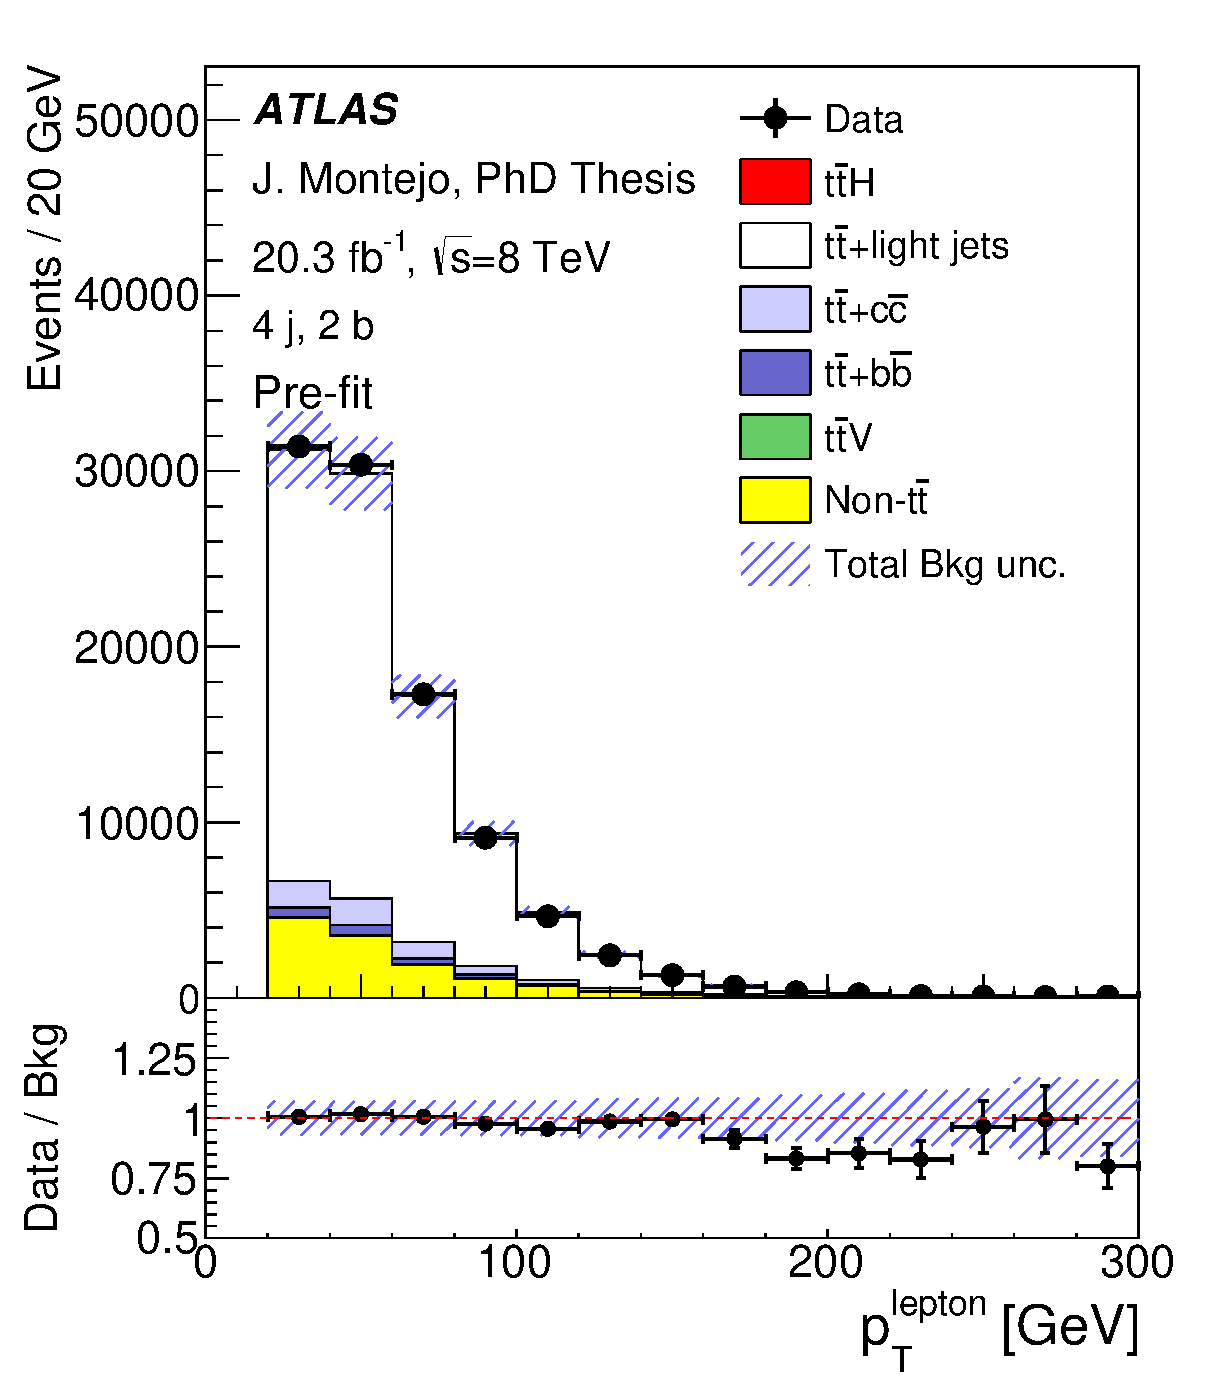
\includegraphics[width=0.27\textwidth]{Analysis/Figures_ttH/tesis_vars/prefit/lep_pt_4jetex2btagex.eps} &
  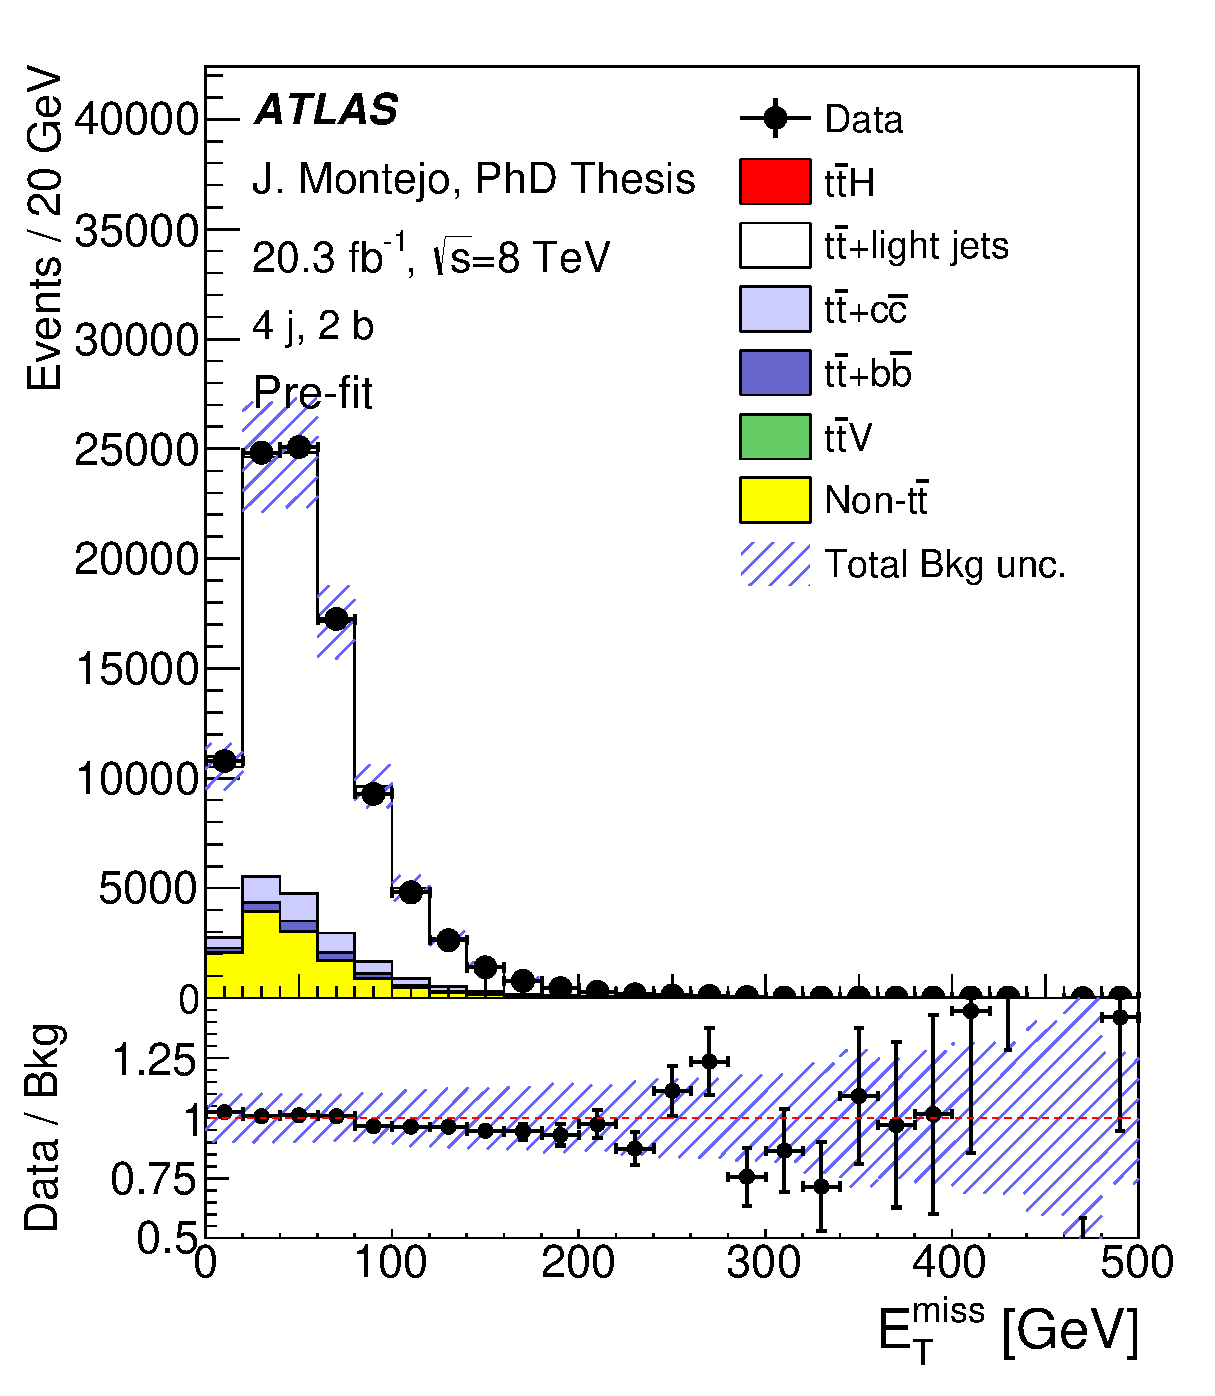
\includegraphics[width=0.27\textwidth]{Analysis/Figures_ttH/tesis_vars/prefit/met_4jetex2btagex.eps} &
  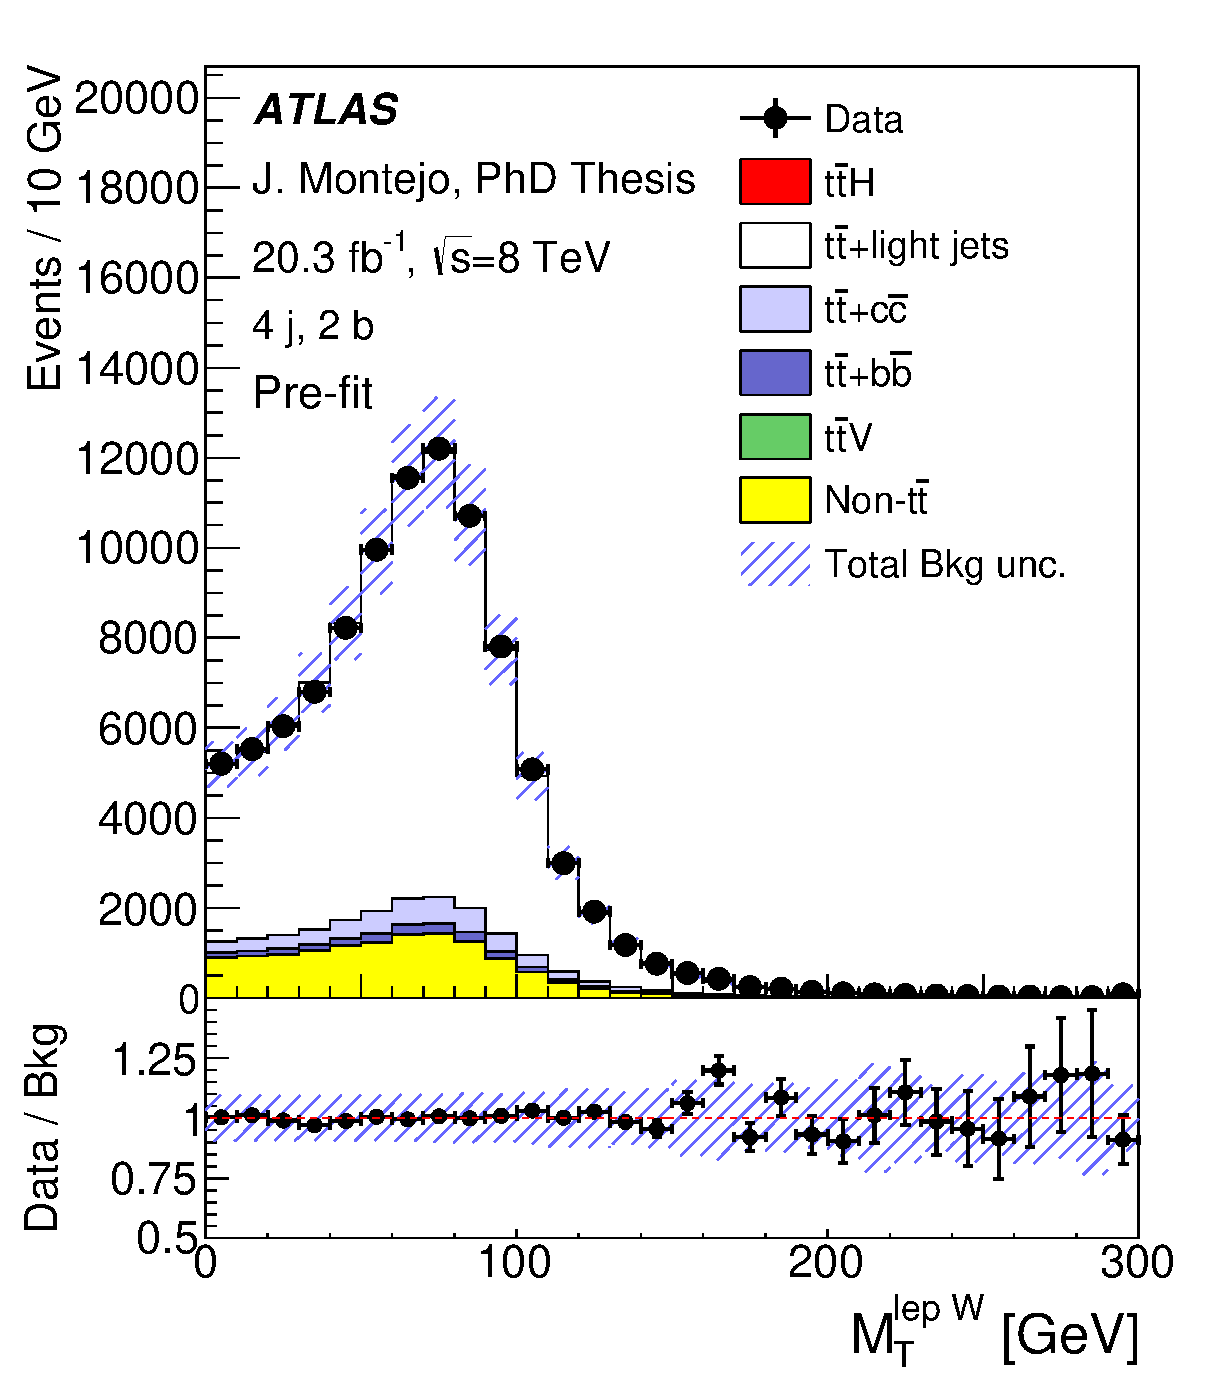
\includegraphics[width=0.27\textwidth]{Analysis/Figures_ttH/tesis_vars/prefit/WlepMT_4jetex2btagex.eps} \\
  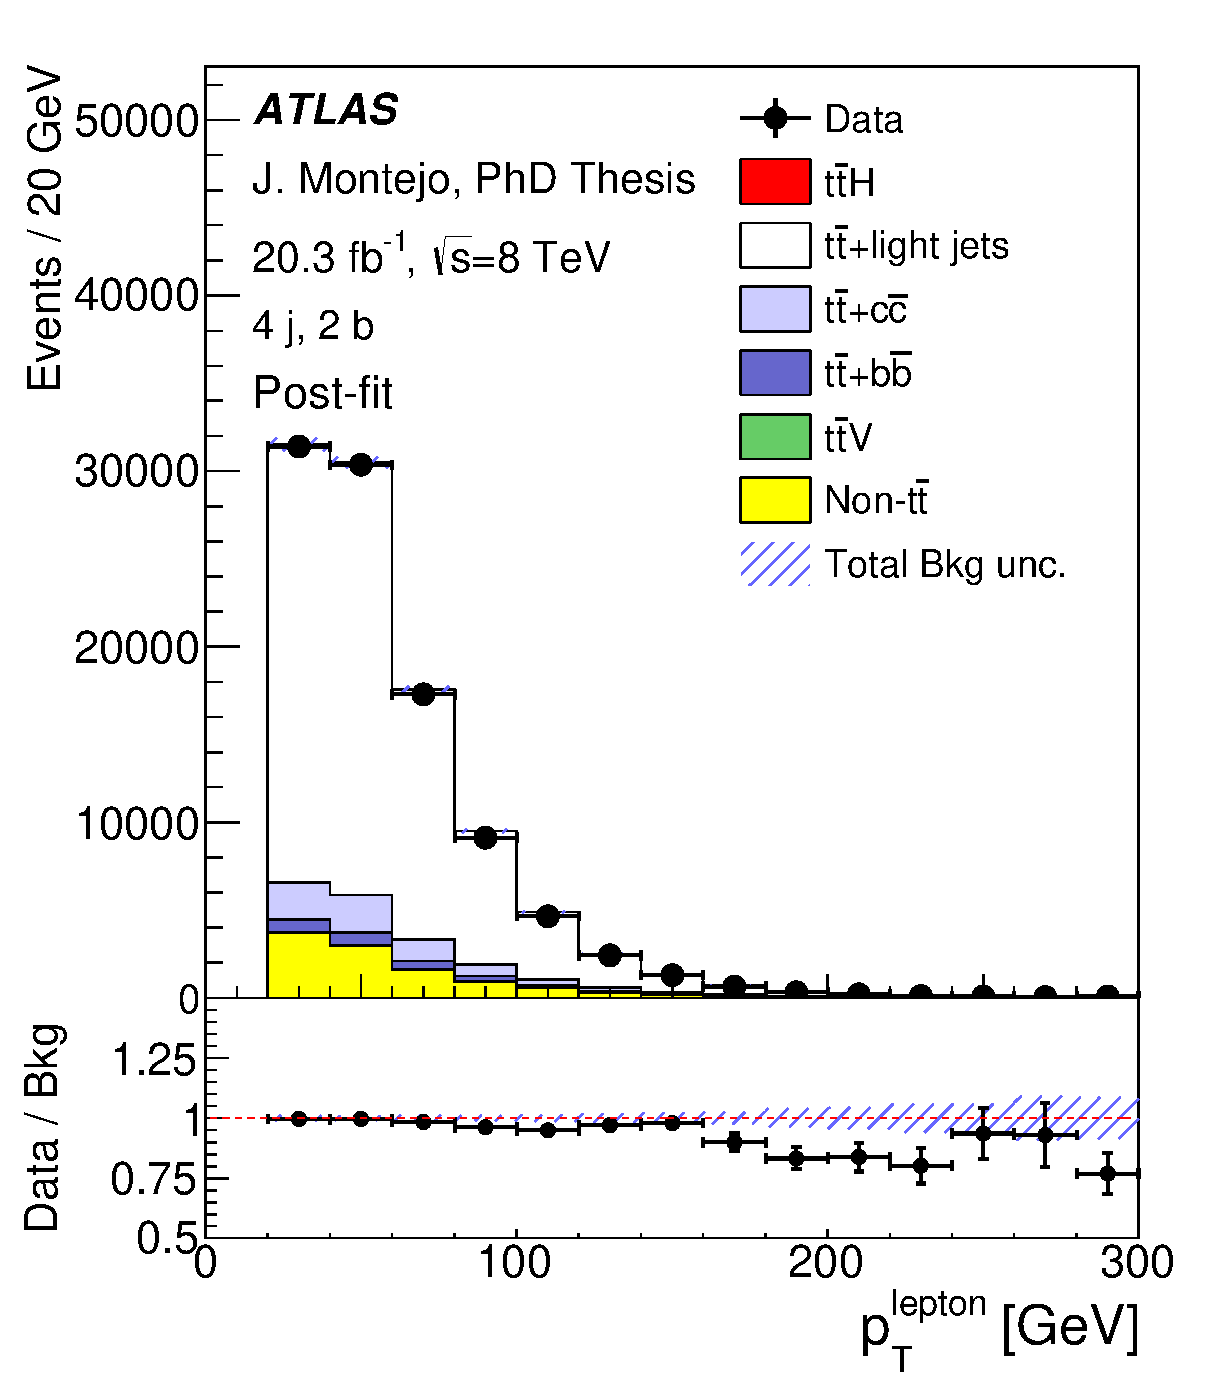
\includegraphics[width=0.27\textwidth]{Analysis/Figures_ttH/tesis_vars/postfit/lep_pt_4jetex2btagex.eps} &
  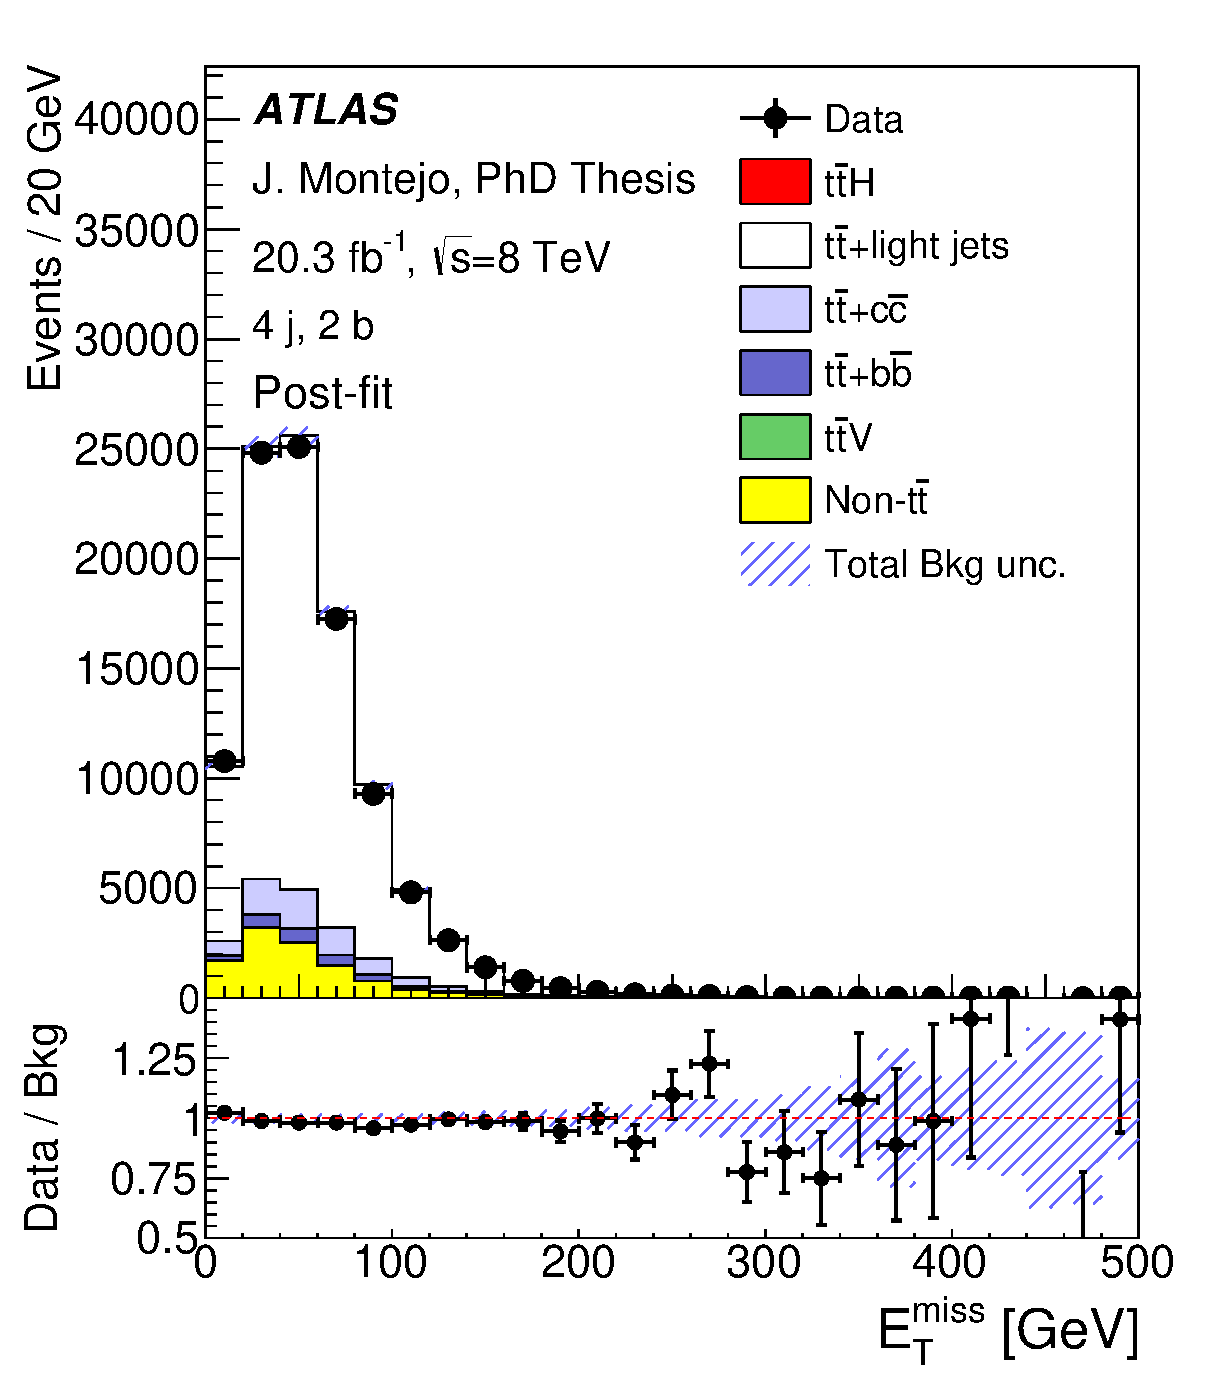
\includegraphics[width=0.27\textwidth]{Analysis/Figures_ttH/tesis_vars/postfit/met_4jetex2btagex.eps} &
  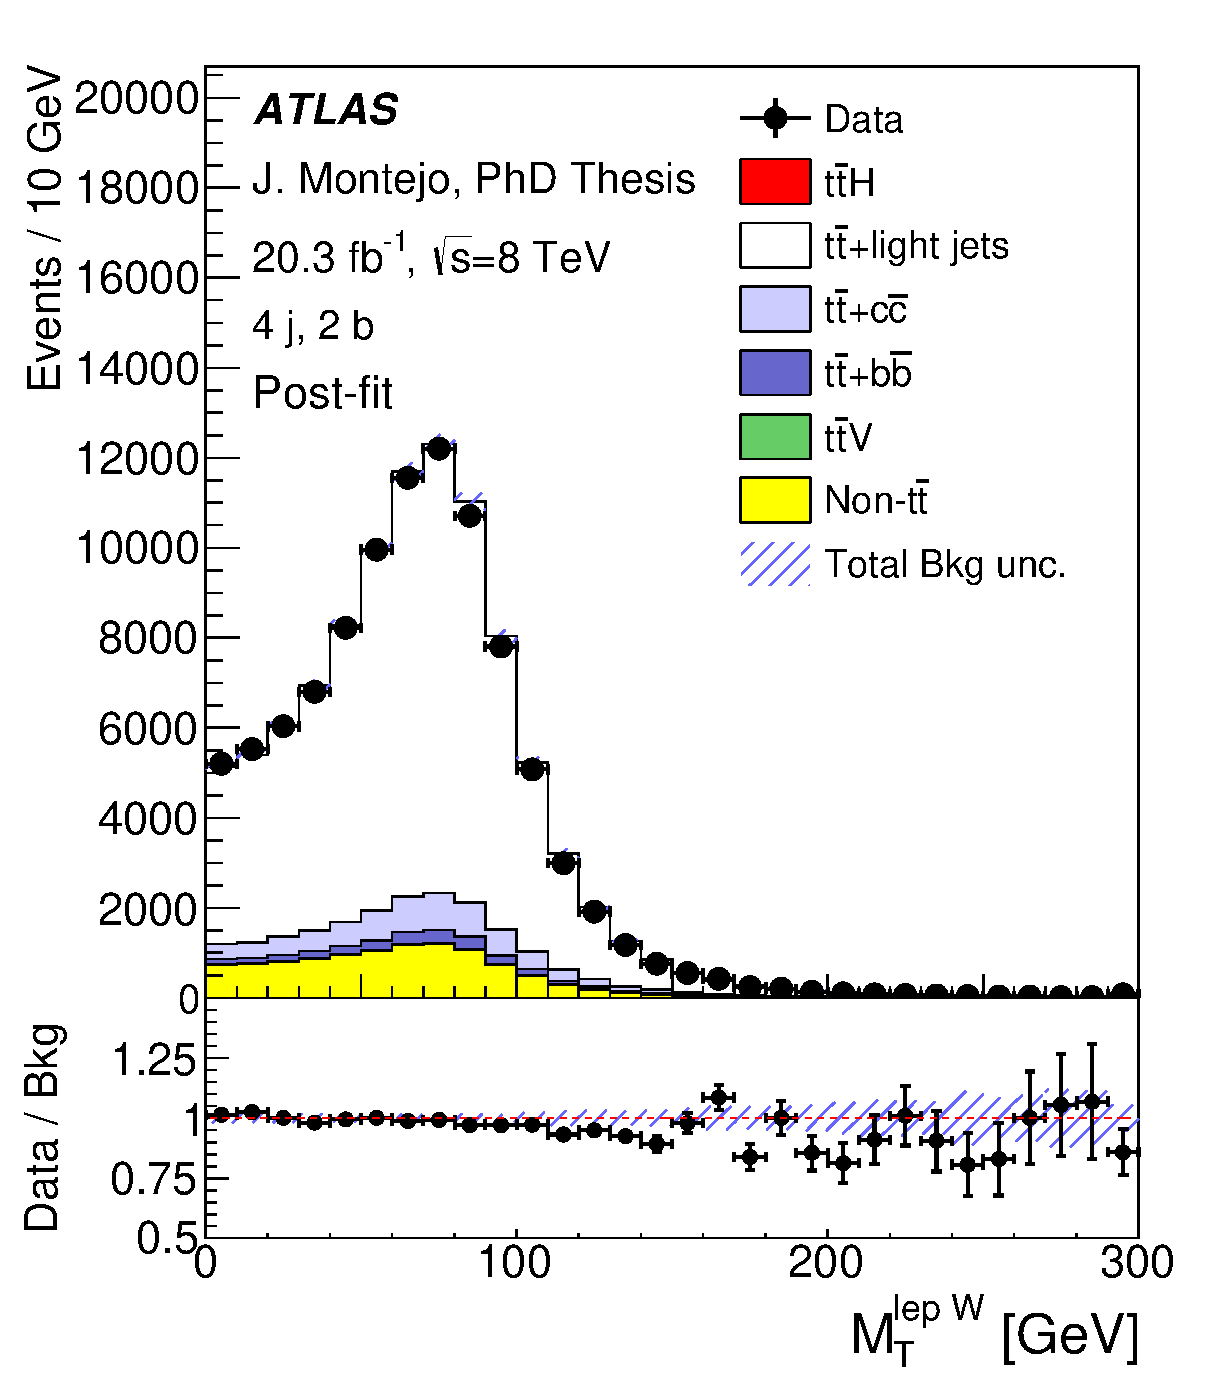
\includegraphics[width=0.27\textwidth]{Analysis/Figures_ttH/tesis_vars/postfit/WlepMT_4jetex2btagex.eps} \\
\end{tabular}
\caption{Comparison between data and prediction in the \fourtwo\ region for (left) lepton \pt,  (middle) missing transverse energy, \met, and (right)  $W$ boson transverse mass, \mtw. The background prediction is shown (top) before the fit and (bottom) after the fit.}
  \label{fig:vars1_fourtwo}
\vspace{0.5cm}
  \centering
  \begin{tabular}{ccc}
  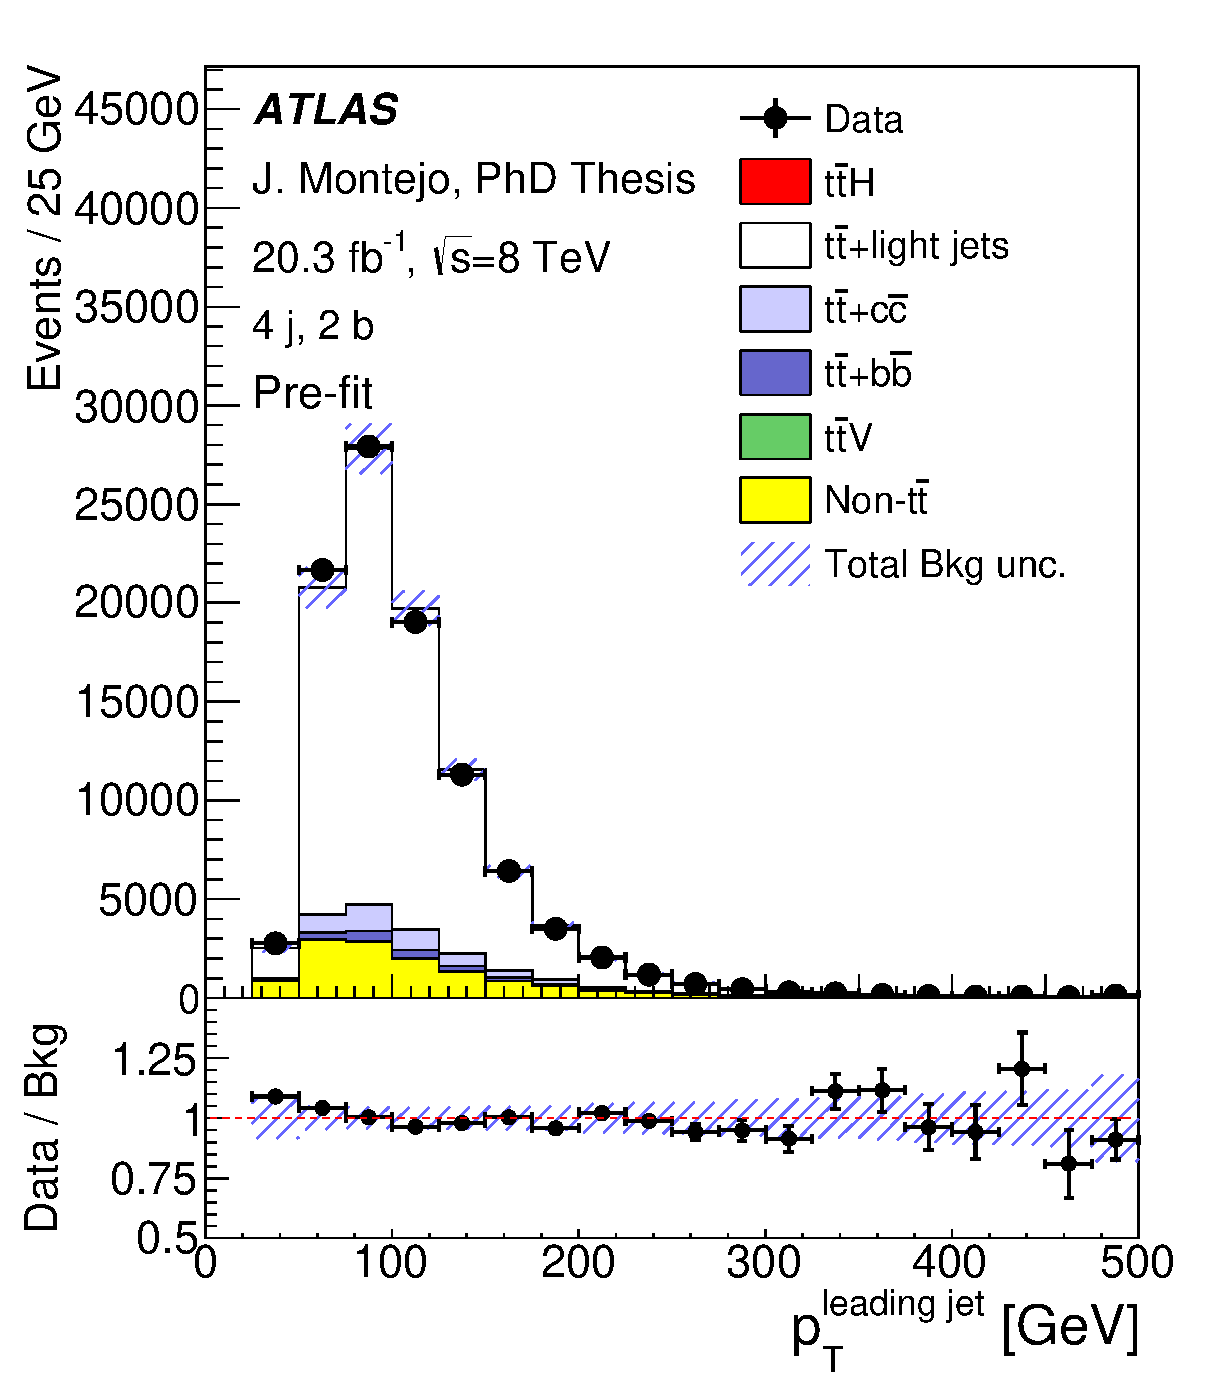
\includegraphics[width=0.27\textwidth]{Analysis/Figures_ttH/tesis_vars/prefit/jet1_pt_4jetex2btagex.eps} &
  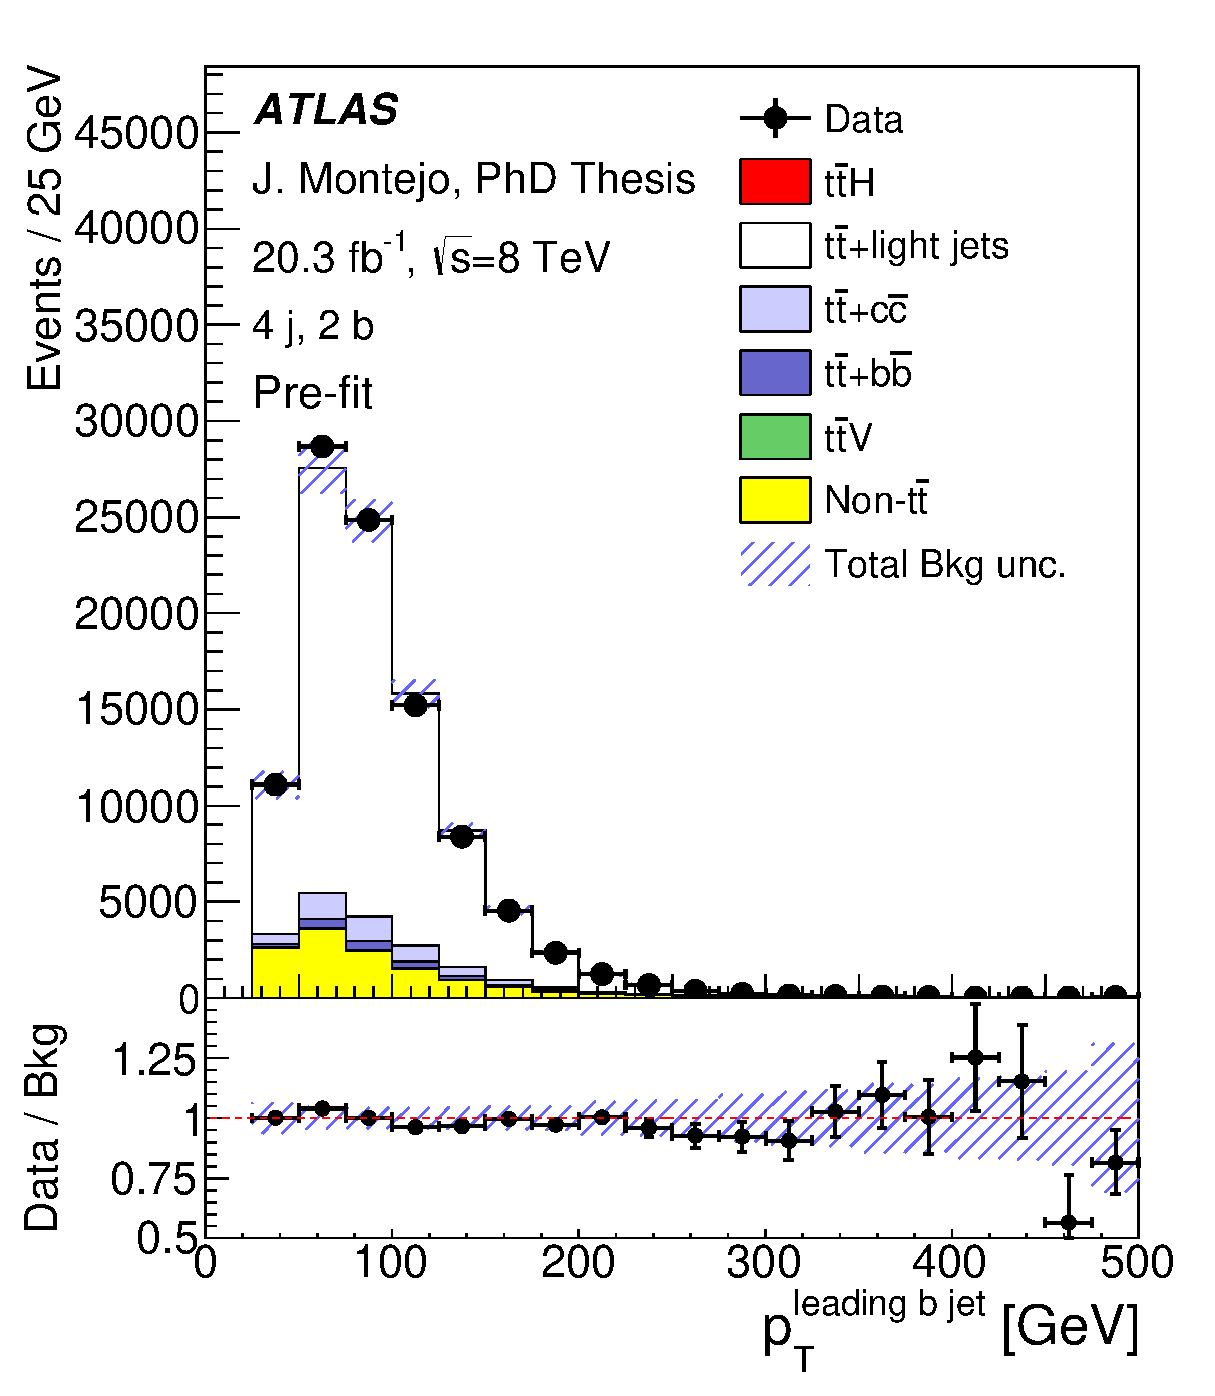
\includegraphics[width=0.27\textwidth]{Analysis/Figures_ttH/tesis_vars/prefit/bjet1_pt_4jetex2btagex.eps} &
  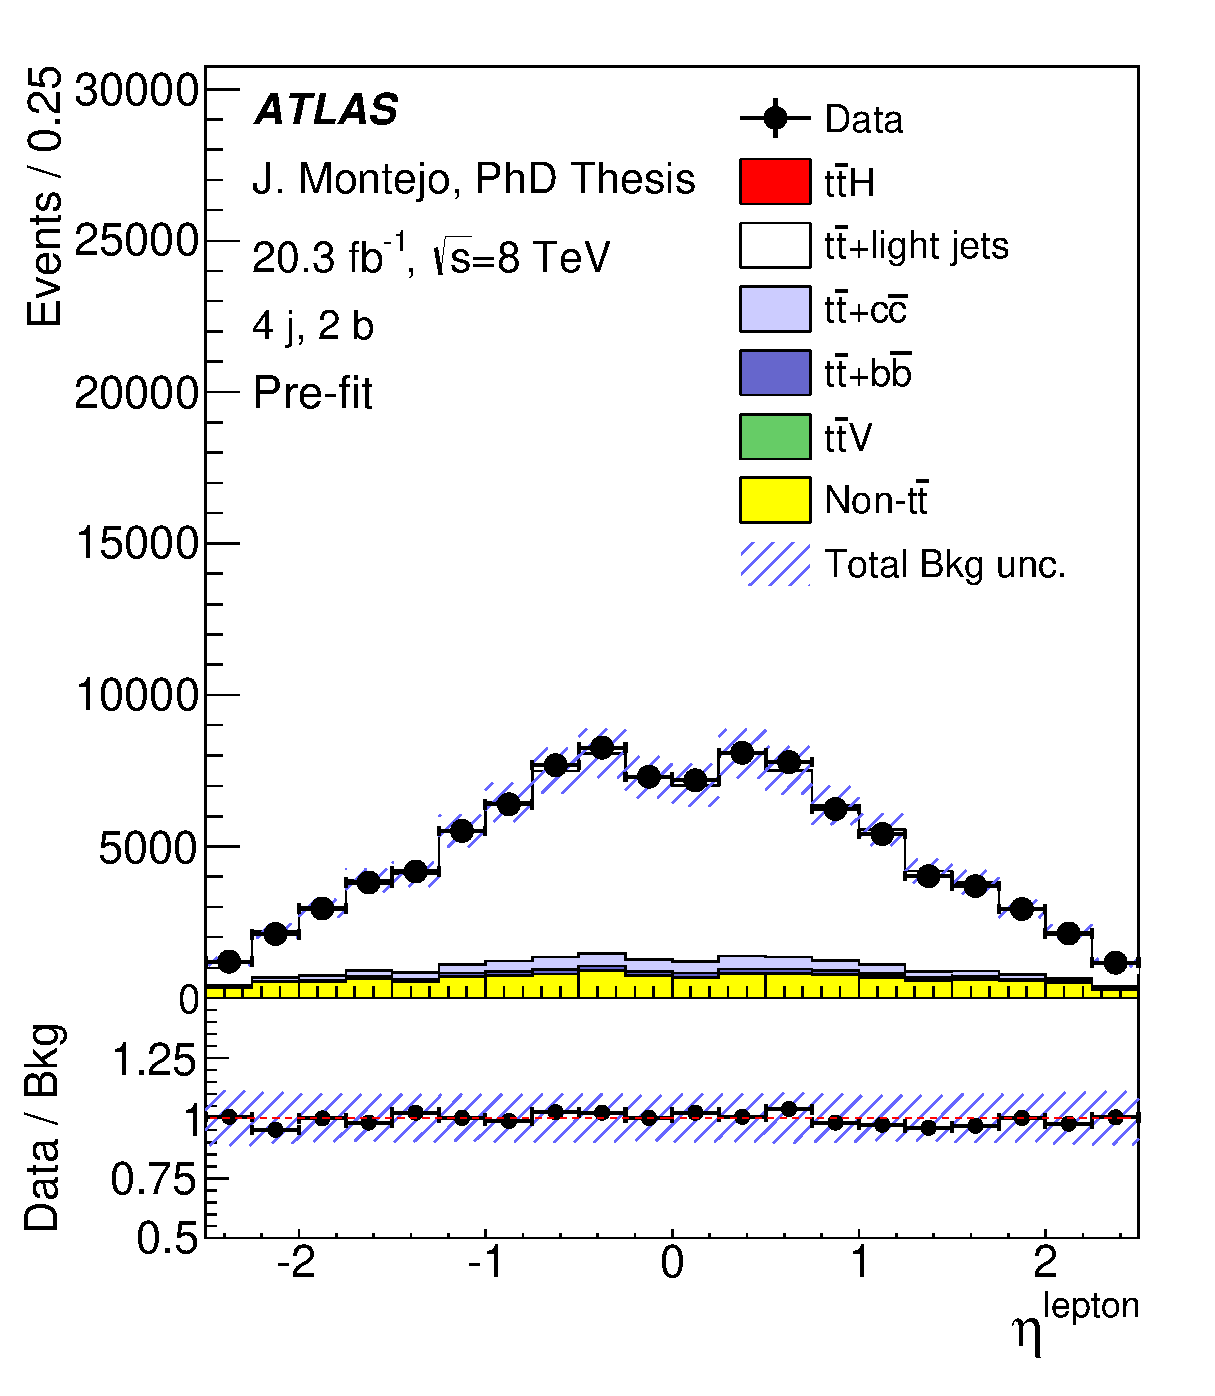
\includegraphics[width=0.27\textwidth]{Analysis/Figures_ttH/tesis_vars/prefit/lep_eta_4jetex2btagex.eps} \\
  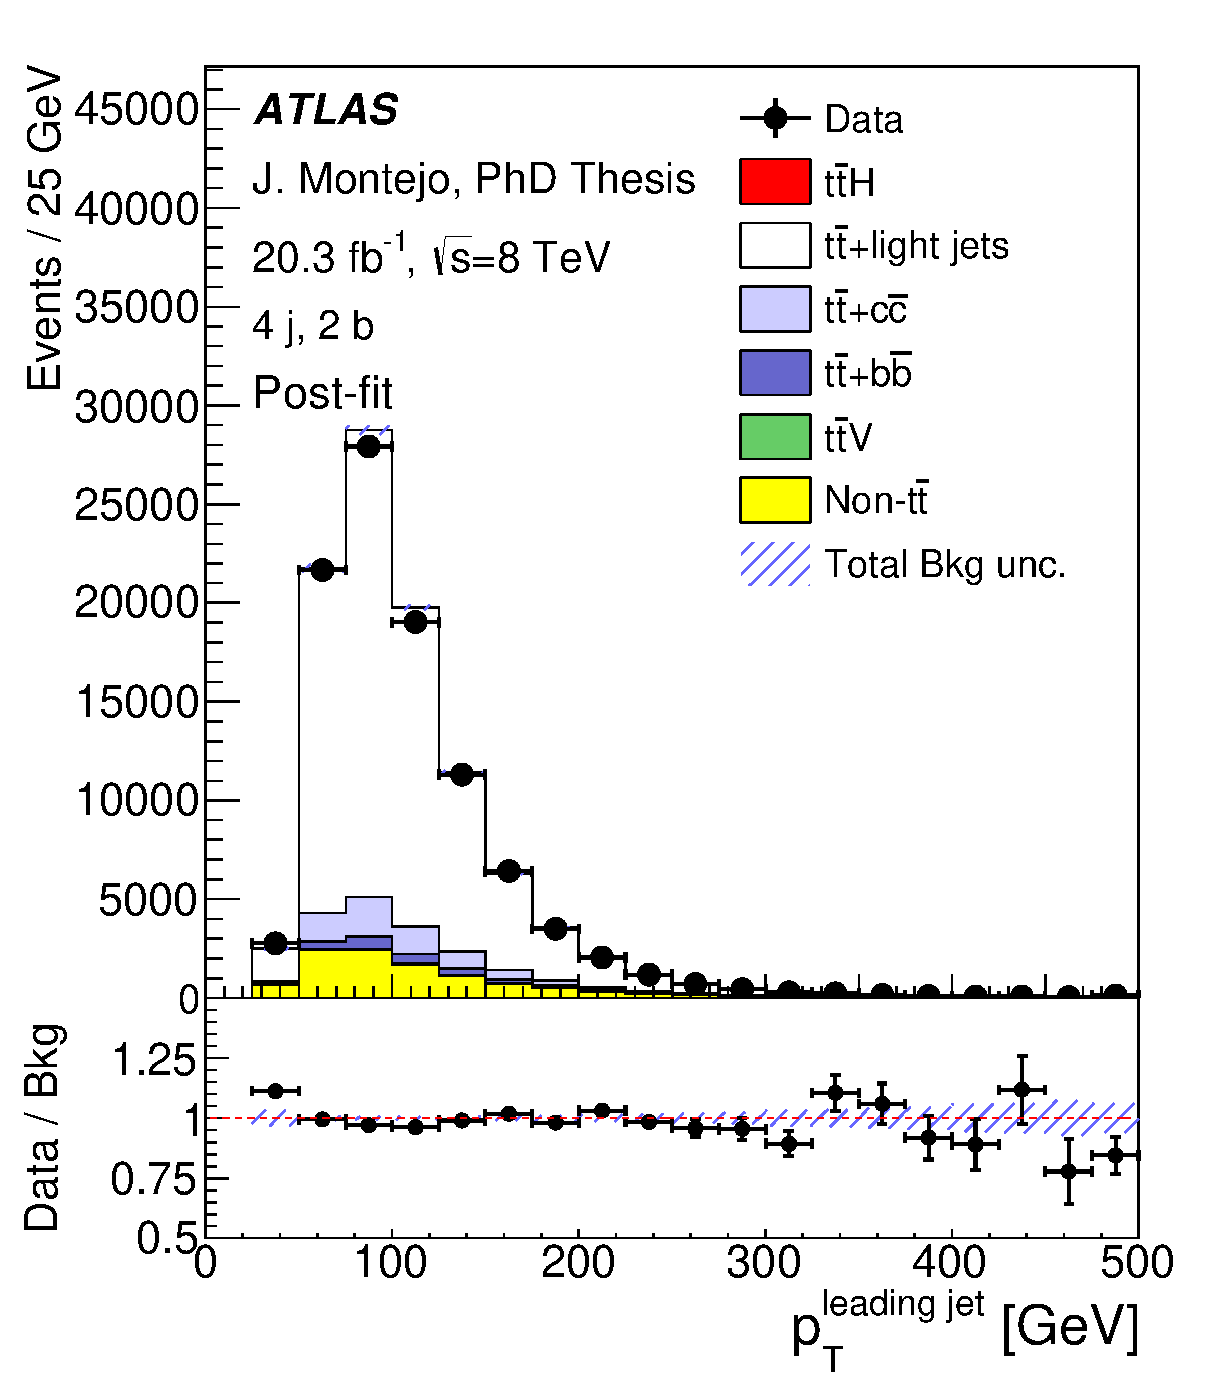
\includegraphics[width=0.27\textwidth]{Analysis/Figures_ttH/tesis_vars/postfit/jet1_pt_4jetex2btagex.eps} &
  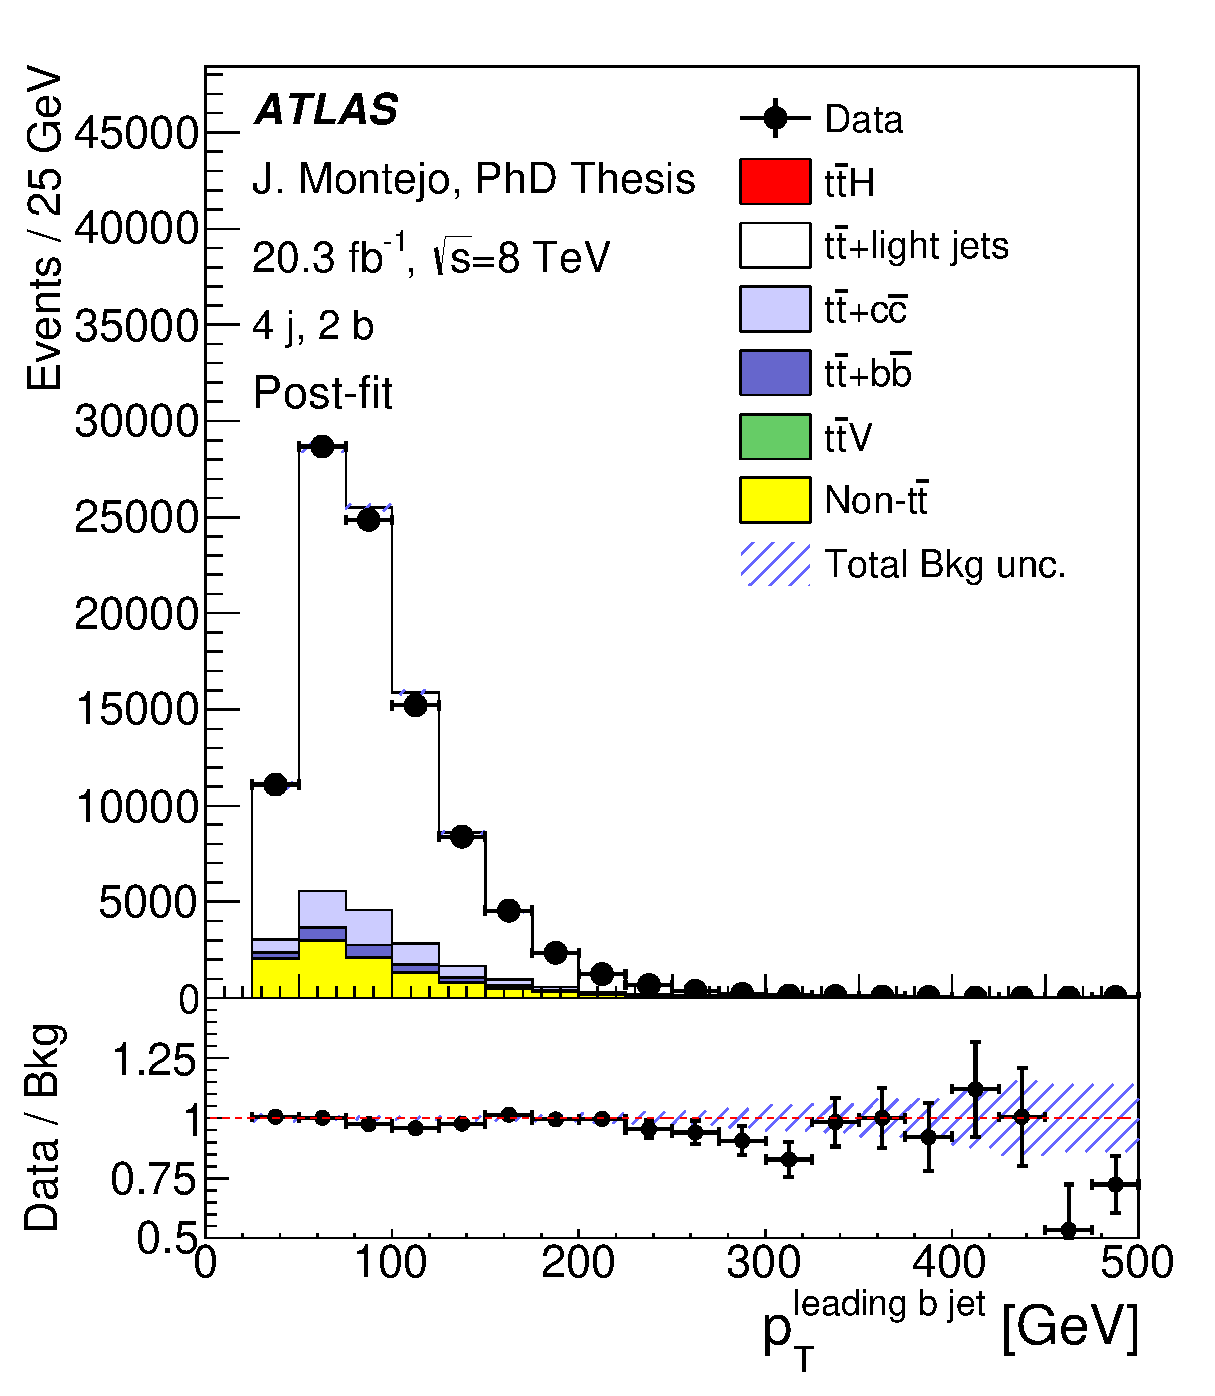
\includegraphics[width=0.27\textwidth]{Analysis/Figures_ttH/tesis_vars/postfit/bjet1_pt_4jetex2btagex.eps} &
  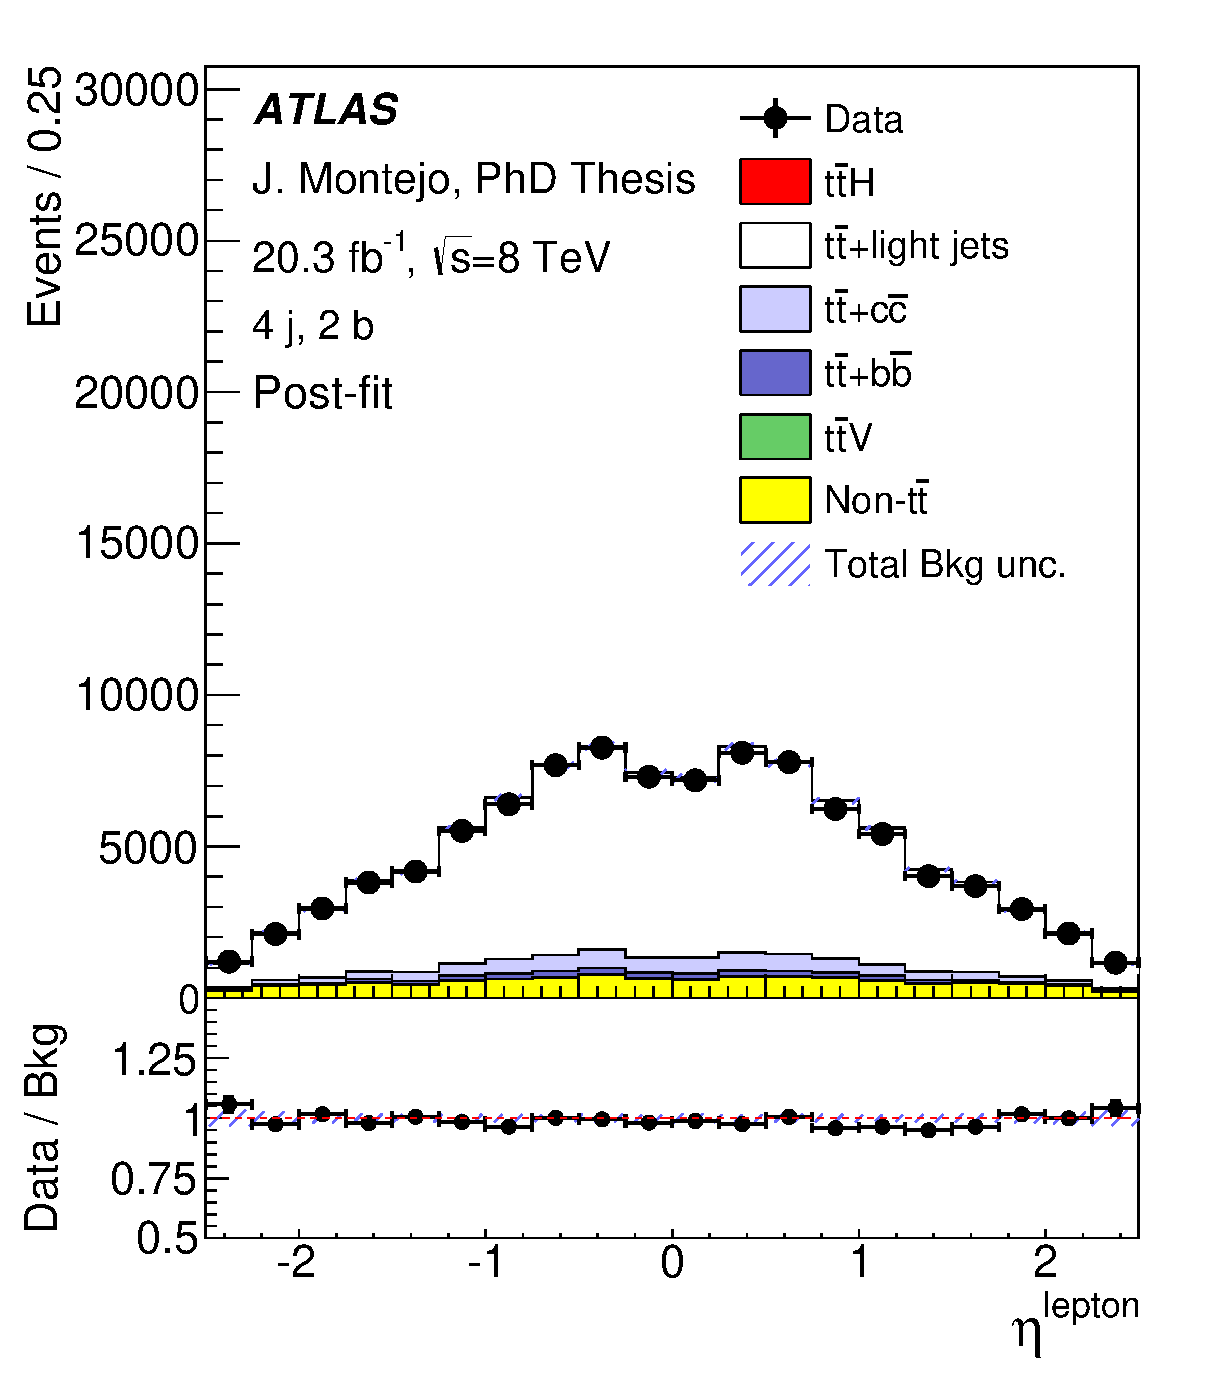
\includegraphics[width=0.27\textwidth]{Analysis/Figures_ttH/tesis_vars/postfit/lep_eta_4jetex2btagex.eps} \\
\end{tabular}
\caption{Comparison between data and prediction in the \fourtwo\ region for (left) leading jet \pt, (middle) leading $b$-tagged jet \pt, (right) lepton pseudo-rapidity. The background prediction is shown (top) before the fit and (bottom) after the fit.}
  \label{fig:vars2_fourtwo}
\end{figure}

\begin{figure}[tp]
  \centering
  \begin{tabular}{ccc}
  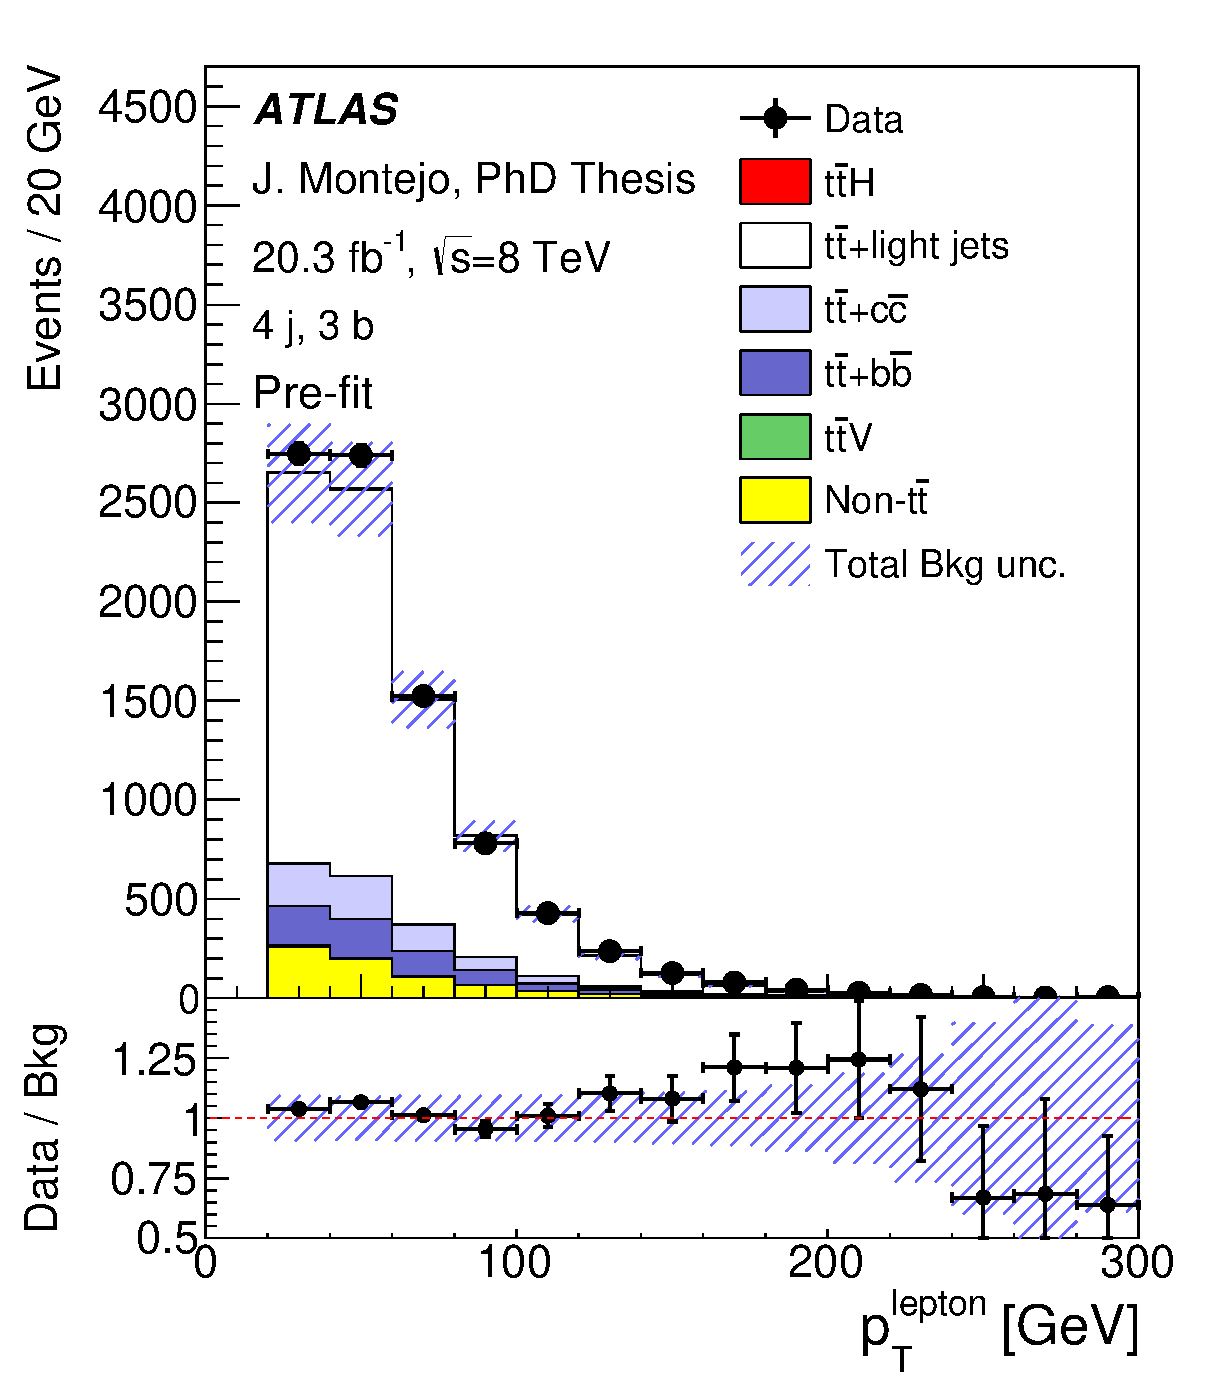
\includegraphics[width=0.27\textwidth]{Analysis/Figures_ttH/tesis_vars/prefit/lep_pt_4jetex3btagex.eps} &
  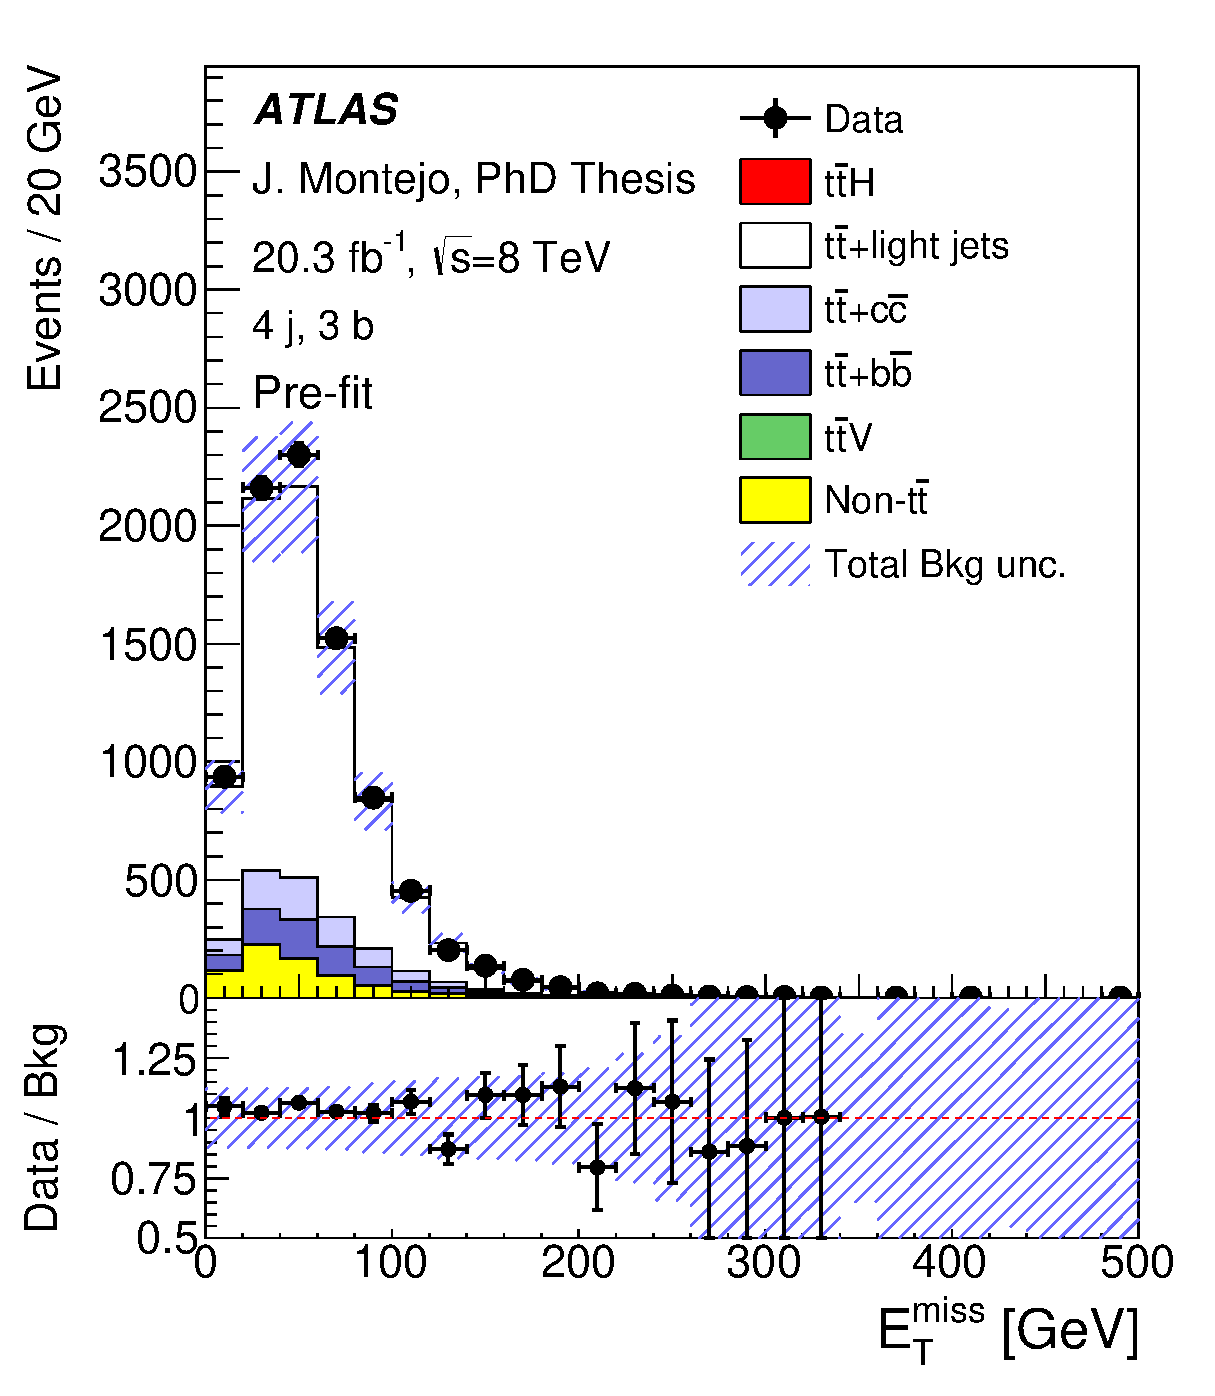
\includegraphics[width=0.27\textwidth]{Analysis/Figures_ttH/tesis_vars/prefit/met_4jetex3btagex.eps} &
  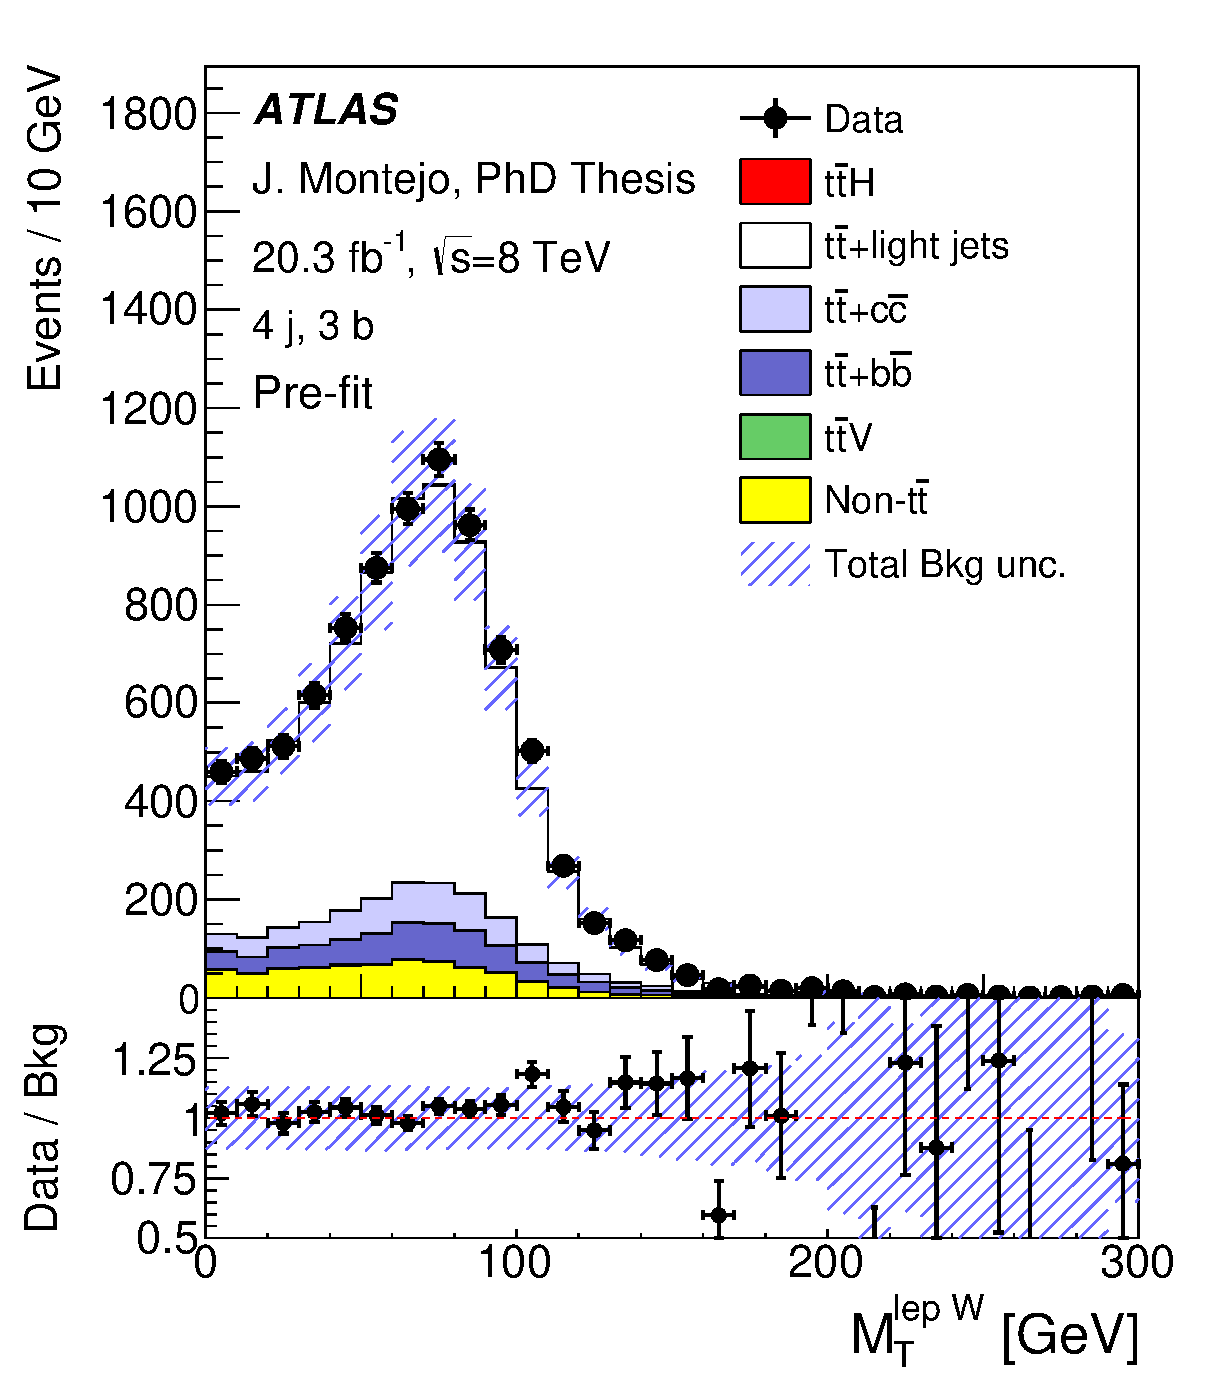
\includegraphics[width=0.27\textwidth]{Analysis/Figures_ttH/tesis_vars/prefit/WlepMT_4jetex3btagex.eps} \\
  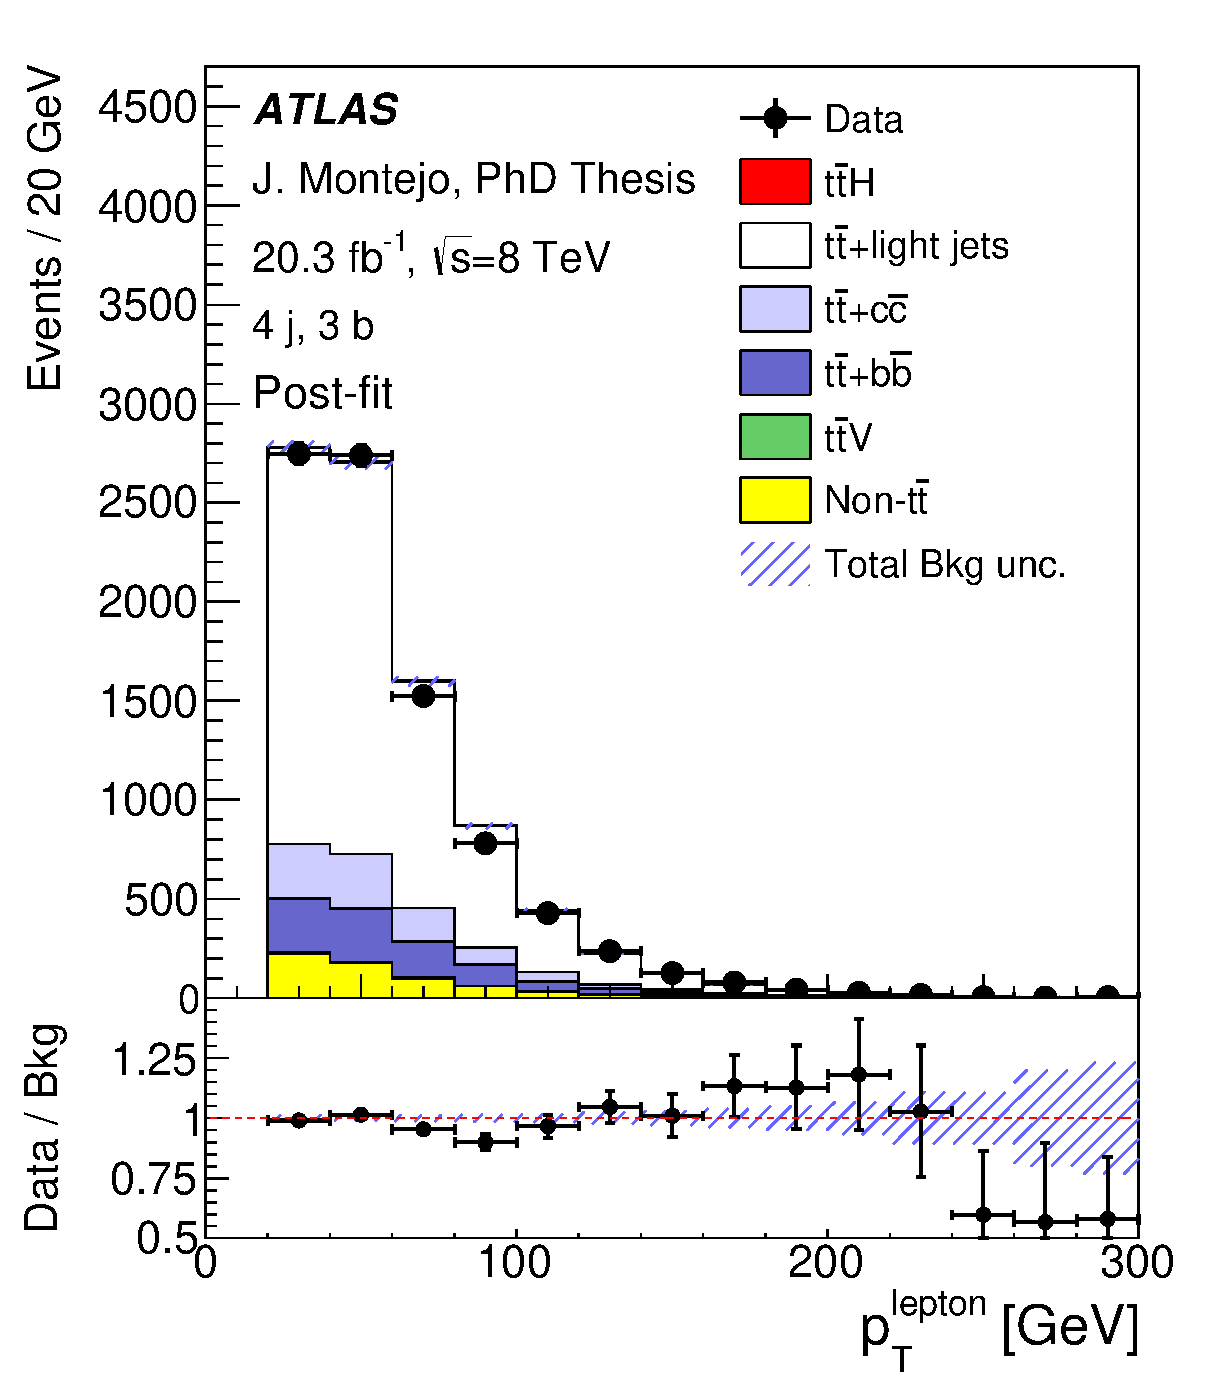
\includegraphics[width=0.27\textwidth]{Analysis/Figures_ttH/tesis_vars/postfit/lep_pt_4jetex3btagex.eps} &
  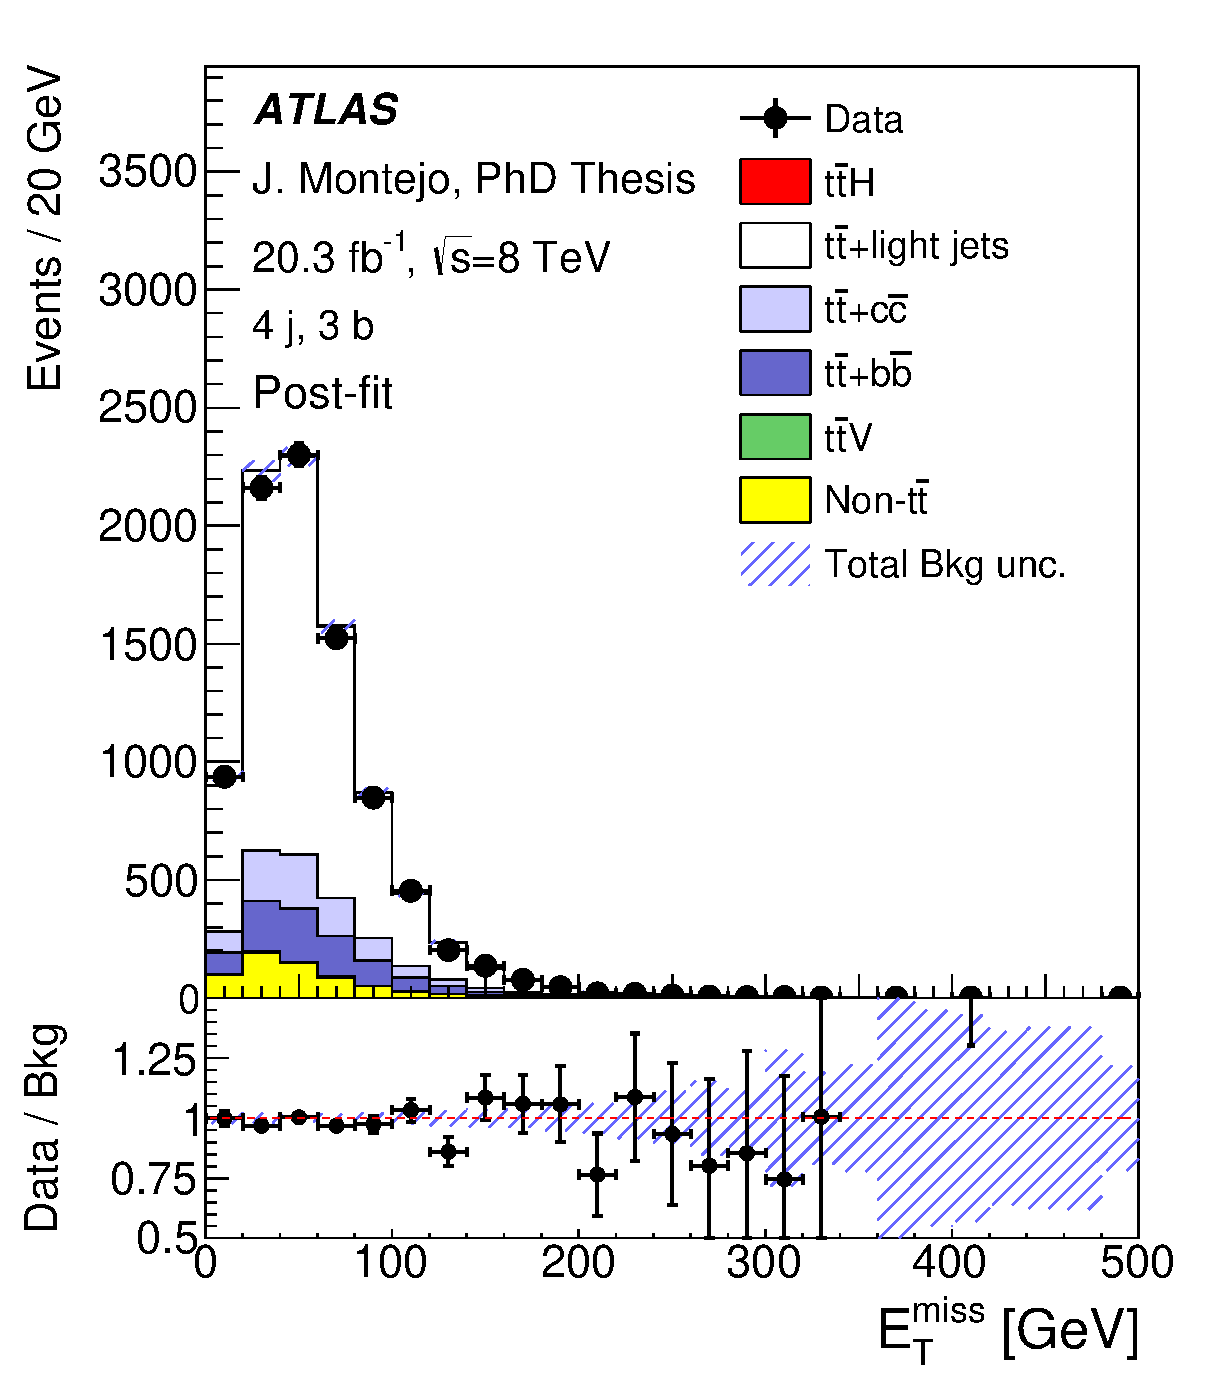
\includegraphics[width=0.27\textwidth]{Analysis/Figures_ttH/tesis_vars/postfit/met_4jetex3btagex.eps} &
  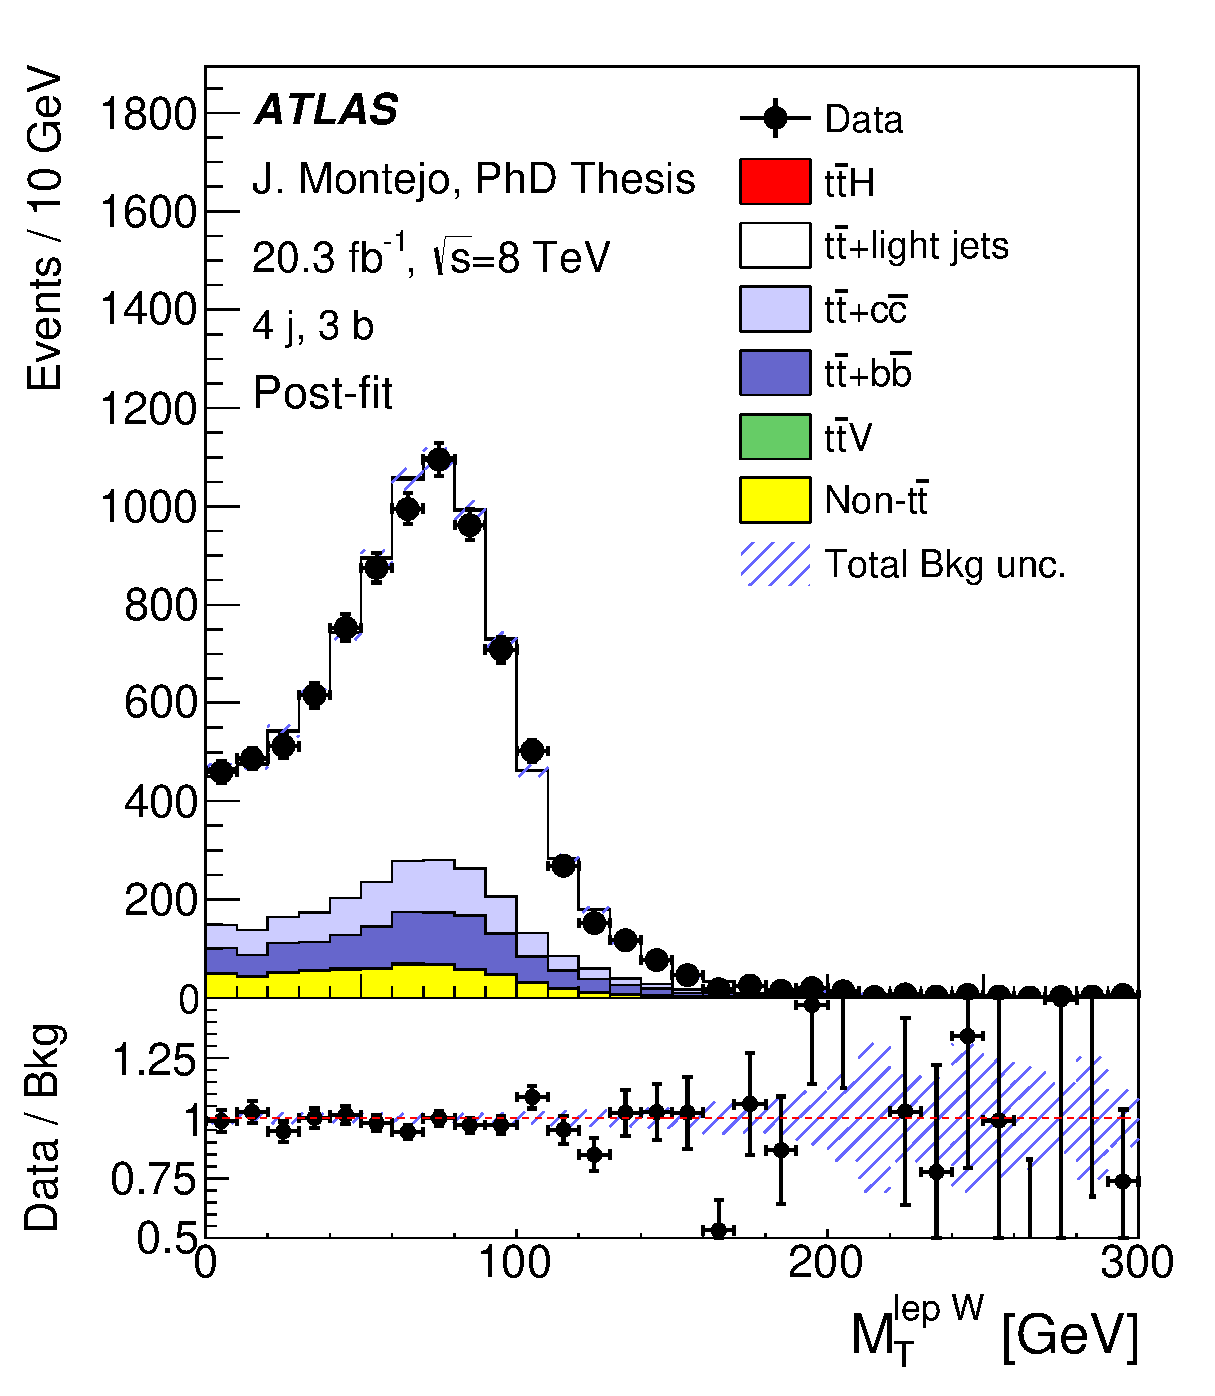
\includegraphics[width=0.27\textwidth]{Analysis/Figures_ttH/tesis_vars/postfit/WlepMT_4jetex3btagex.eps} \\
\end{tabular}
\caption{Comparison between data and prediction in the \fourthree\ region for (left) lepton \pt,  (middle) missing transverse energy, \met, and (right)  $W$ boson transverse mass, \mtw. The background prediction is shown (top) before the fit and (bottom) after the fit.}
  \label{fig:vars1_fourthree}
\vspace{0.5cm}
  \centering
  \begin{tabular}{ccc}
  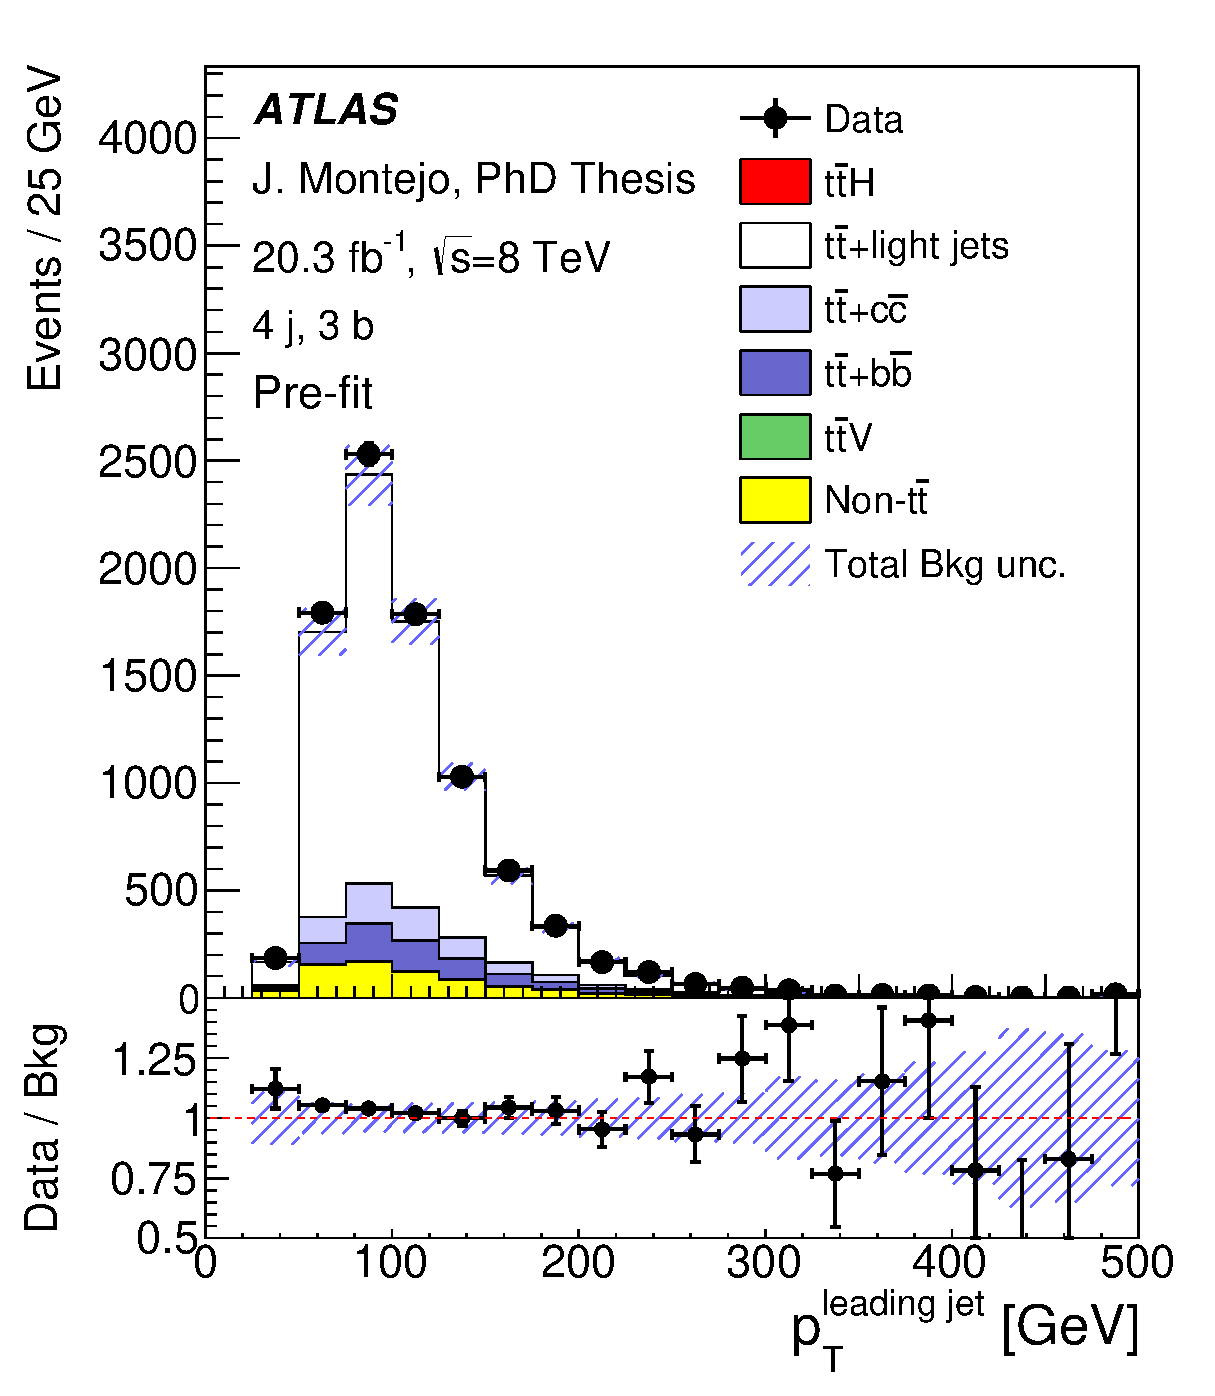
\includegraphics[width=0.27\textwidth]{Analysis/Figures_ttH/tesis_vars/prefit/jet1_pt_4jetex3btagex.eps} &
  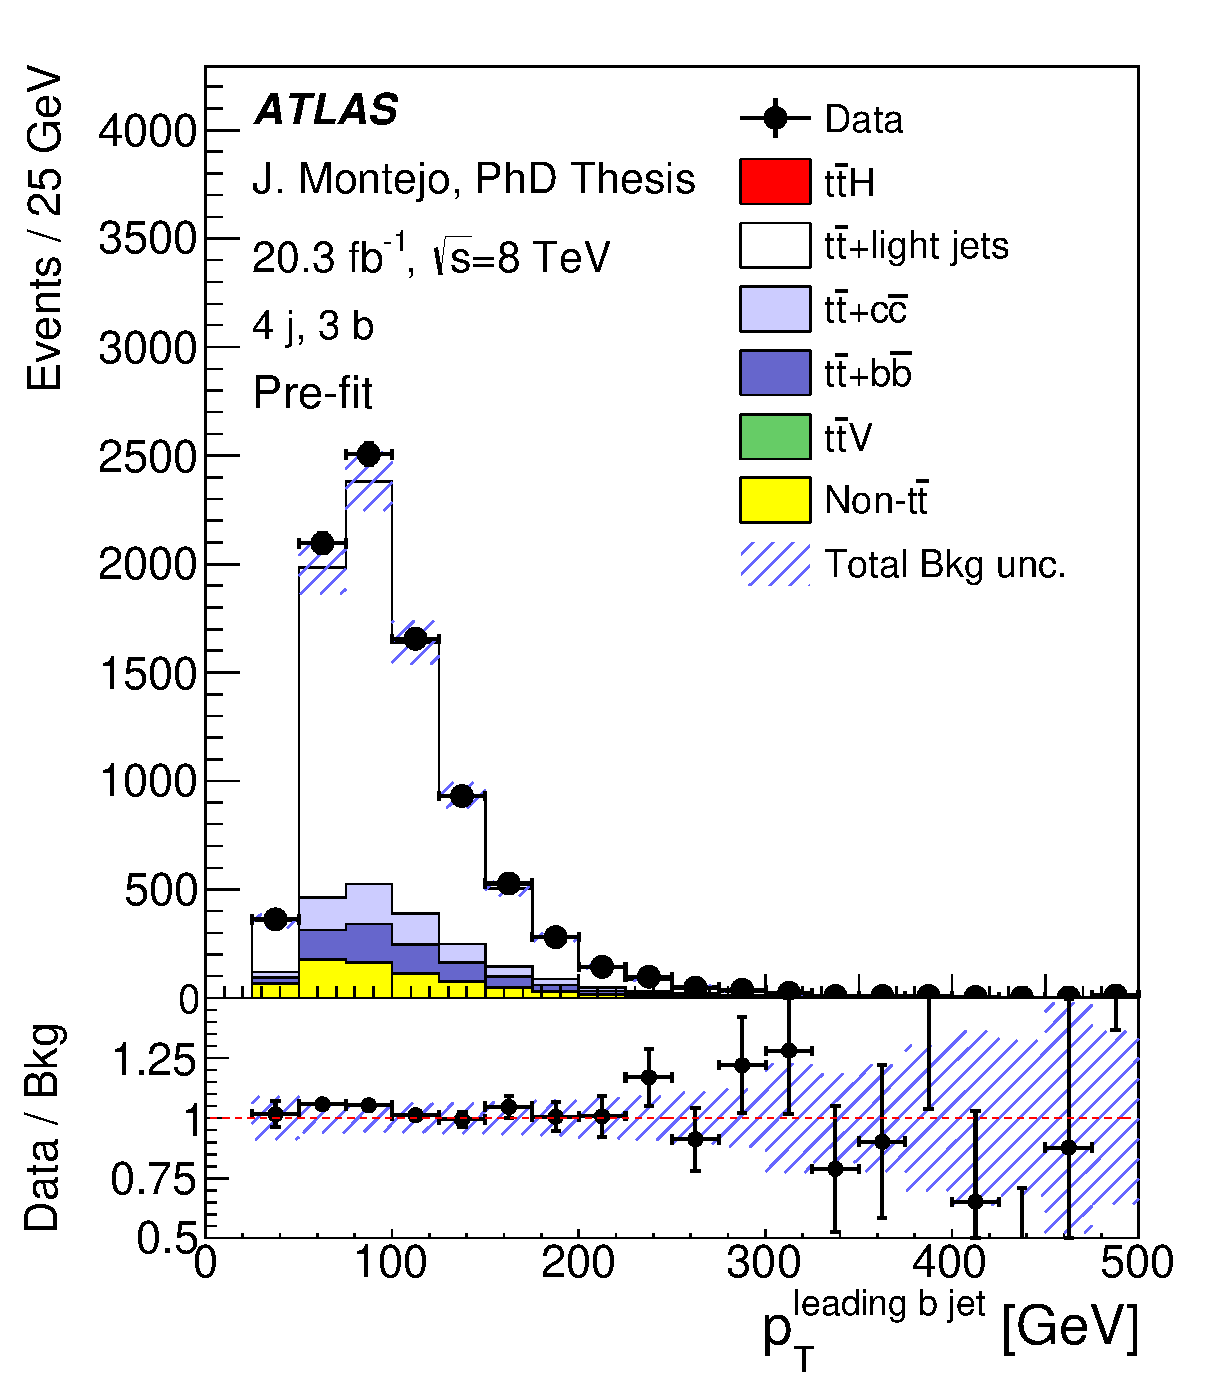
\includegraphics[width=0.27\textwidth]{Analysis/Figures_ttH/tesis_vars/prefit/bjet1_pt_4jetex3btagex.eps} &
  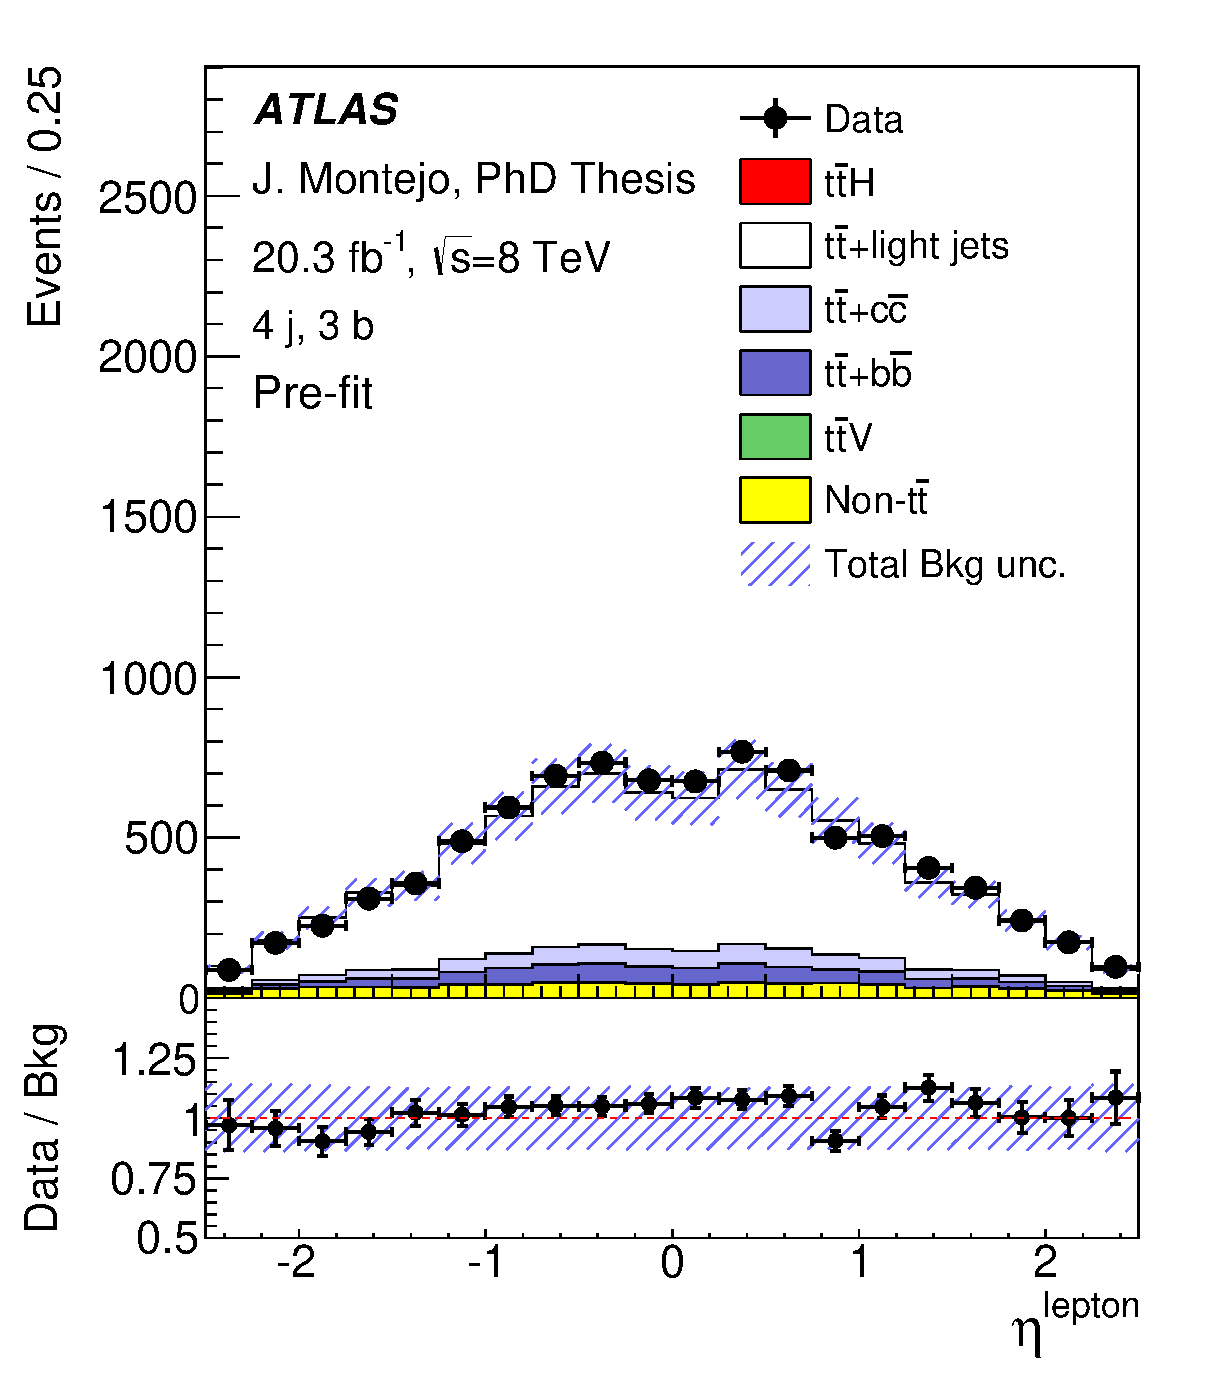
\includegraphics[width=0.27\textwidth]{Analysis/Figures_ttH/tesis_vars/prefit/lep_eta_4jetex3btagex.eps} \\
  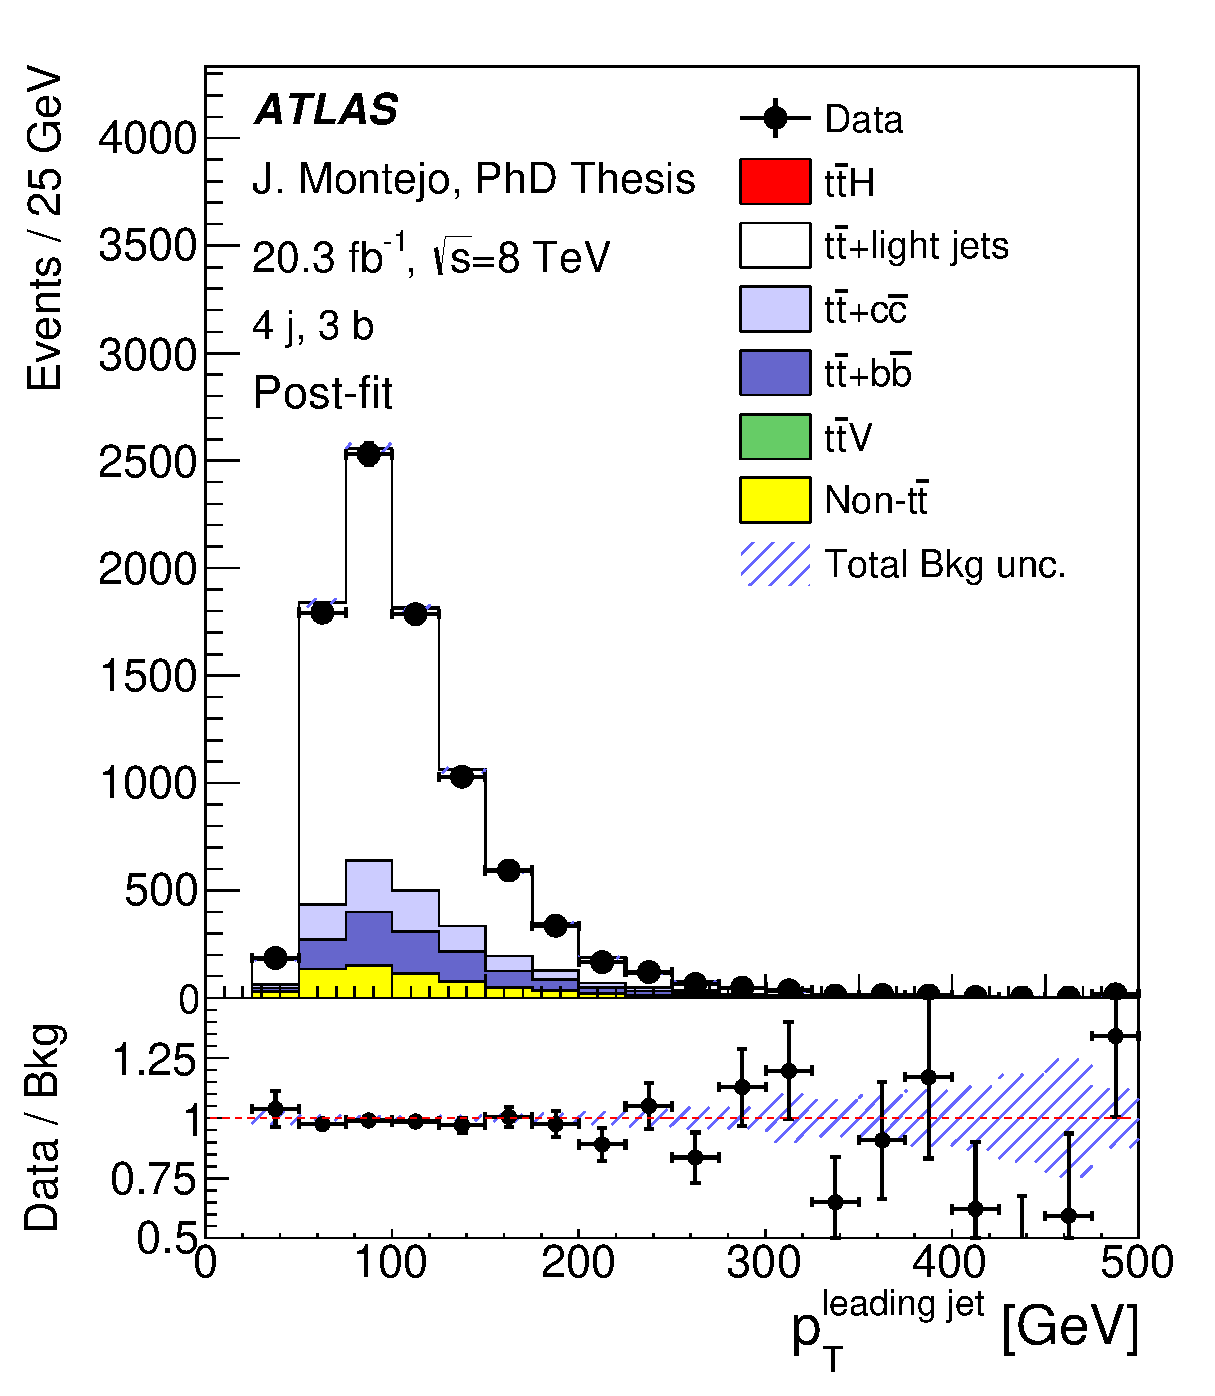
\includegraphics[width=0.27\textwidth]{Analysis/Figures_ttH/tesis_vars/postfit/jet1_pt_4jetex3btagex.eps} &
  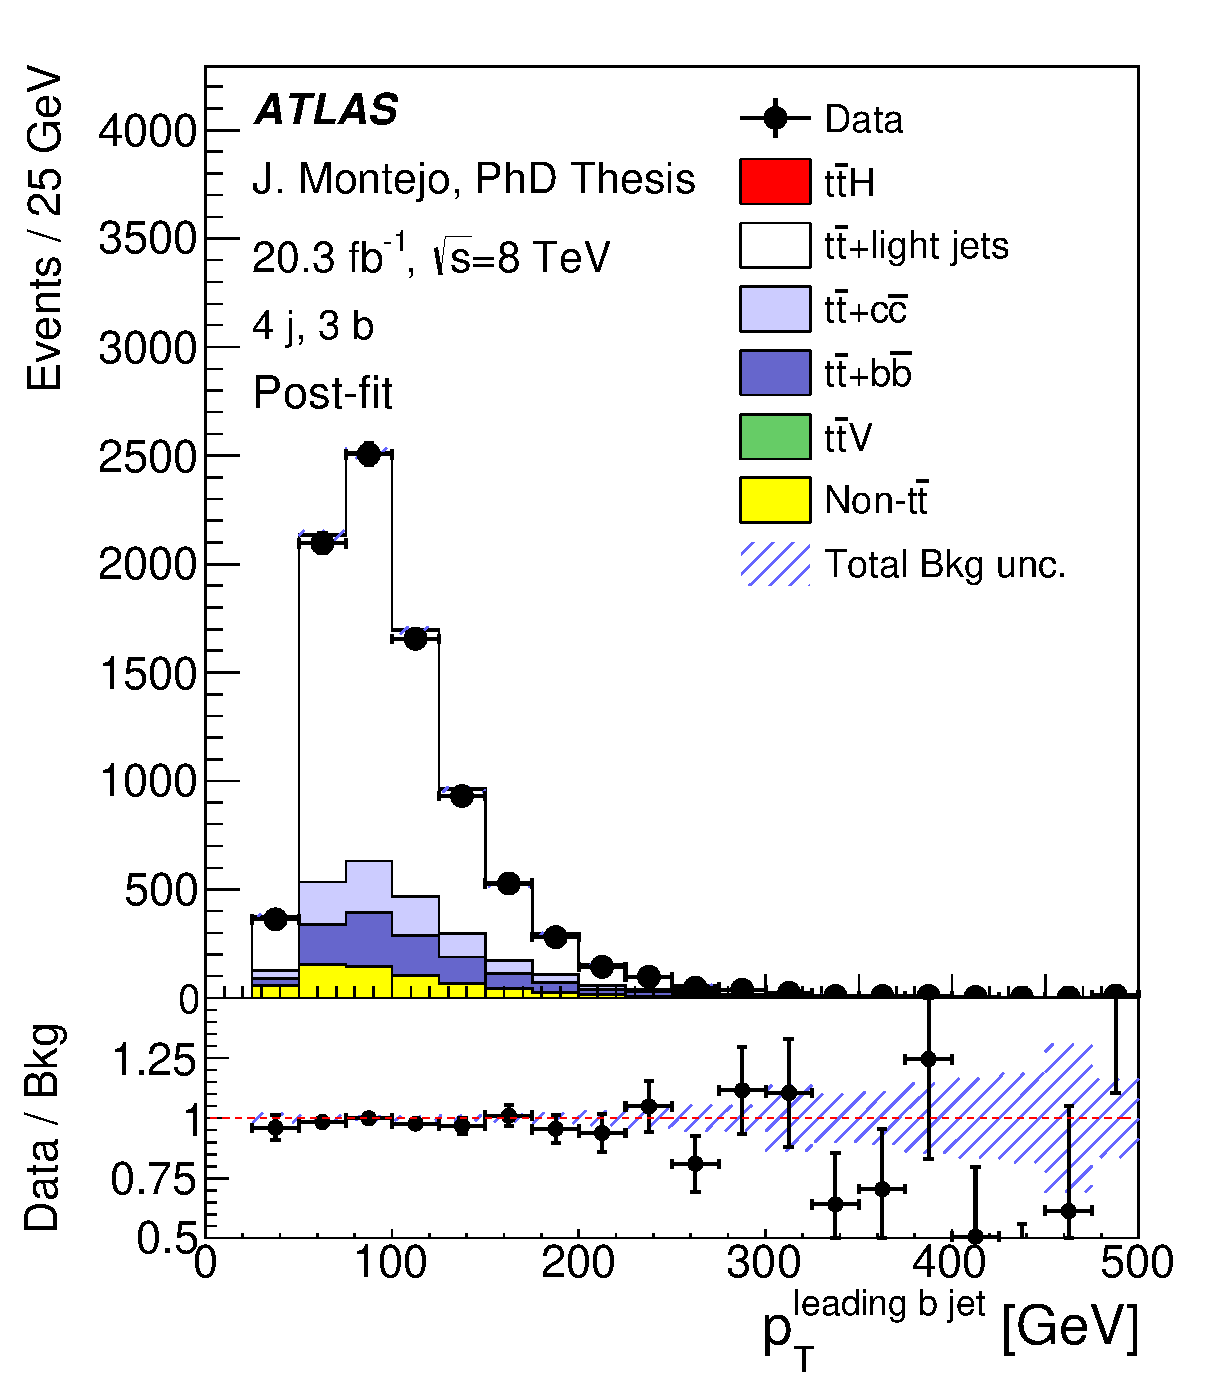
\includegraphics[width=0.27\textwidth]{Analysis/Figures_ttH/tesis_vars/postfit/bjet1_pt_4jetex3btagex.eps} &
  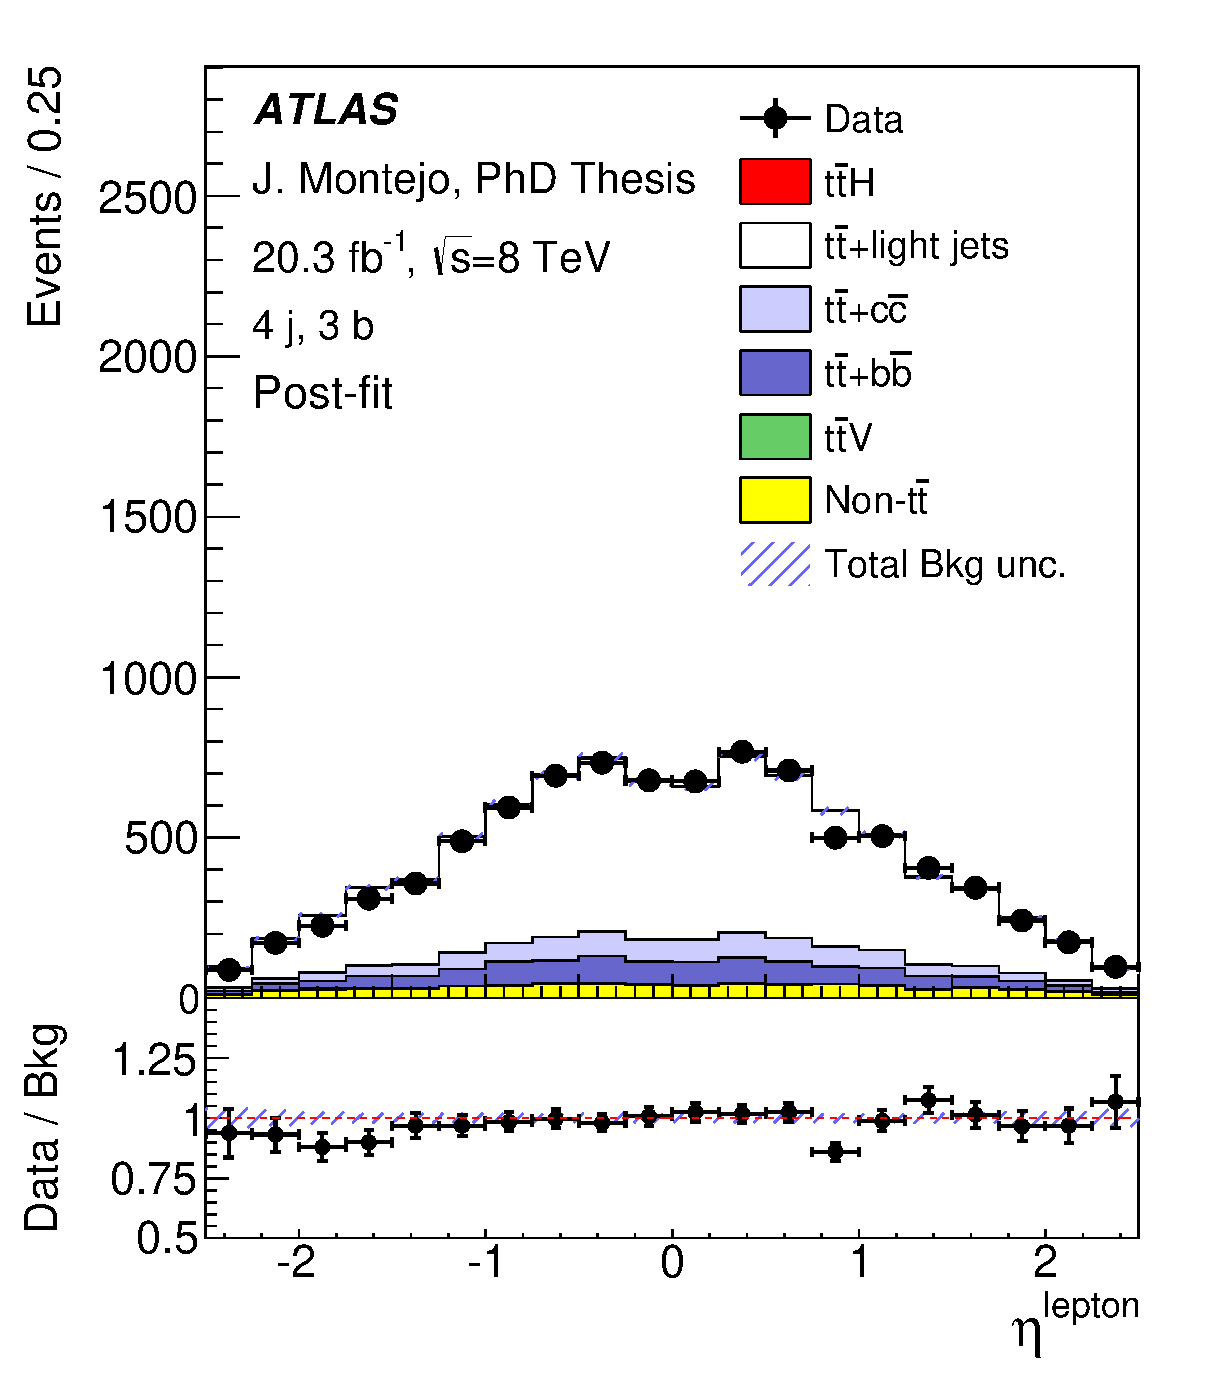
\includegraphics[width=0.27\textwidth]{Analysis/Figures_ttH/tesis_vars/postfit/lep_eta_4jetex3btagex.eps} \\
\end{tabular}
\caption{Comparison between data and prediction in the \fourthree\ region for (left) leading jet \pt, (middle) leading $b$-tagged jet \pt, (right) lepton pseudo-rapidity. The background prediction is shown (top) before the fit and (bottom) after the fit.}
  \label{fig:vars2_fourthree}
\end{figure}
\begin{figure}[tp]
  \centering
  \begin{tabular}{ccc}
  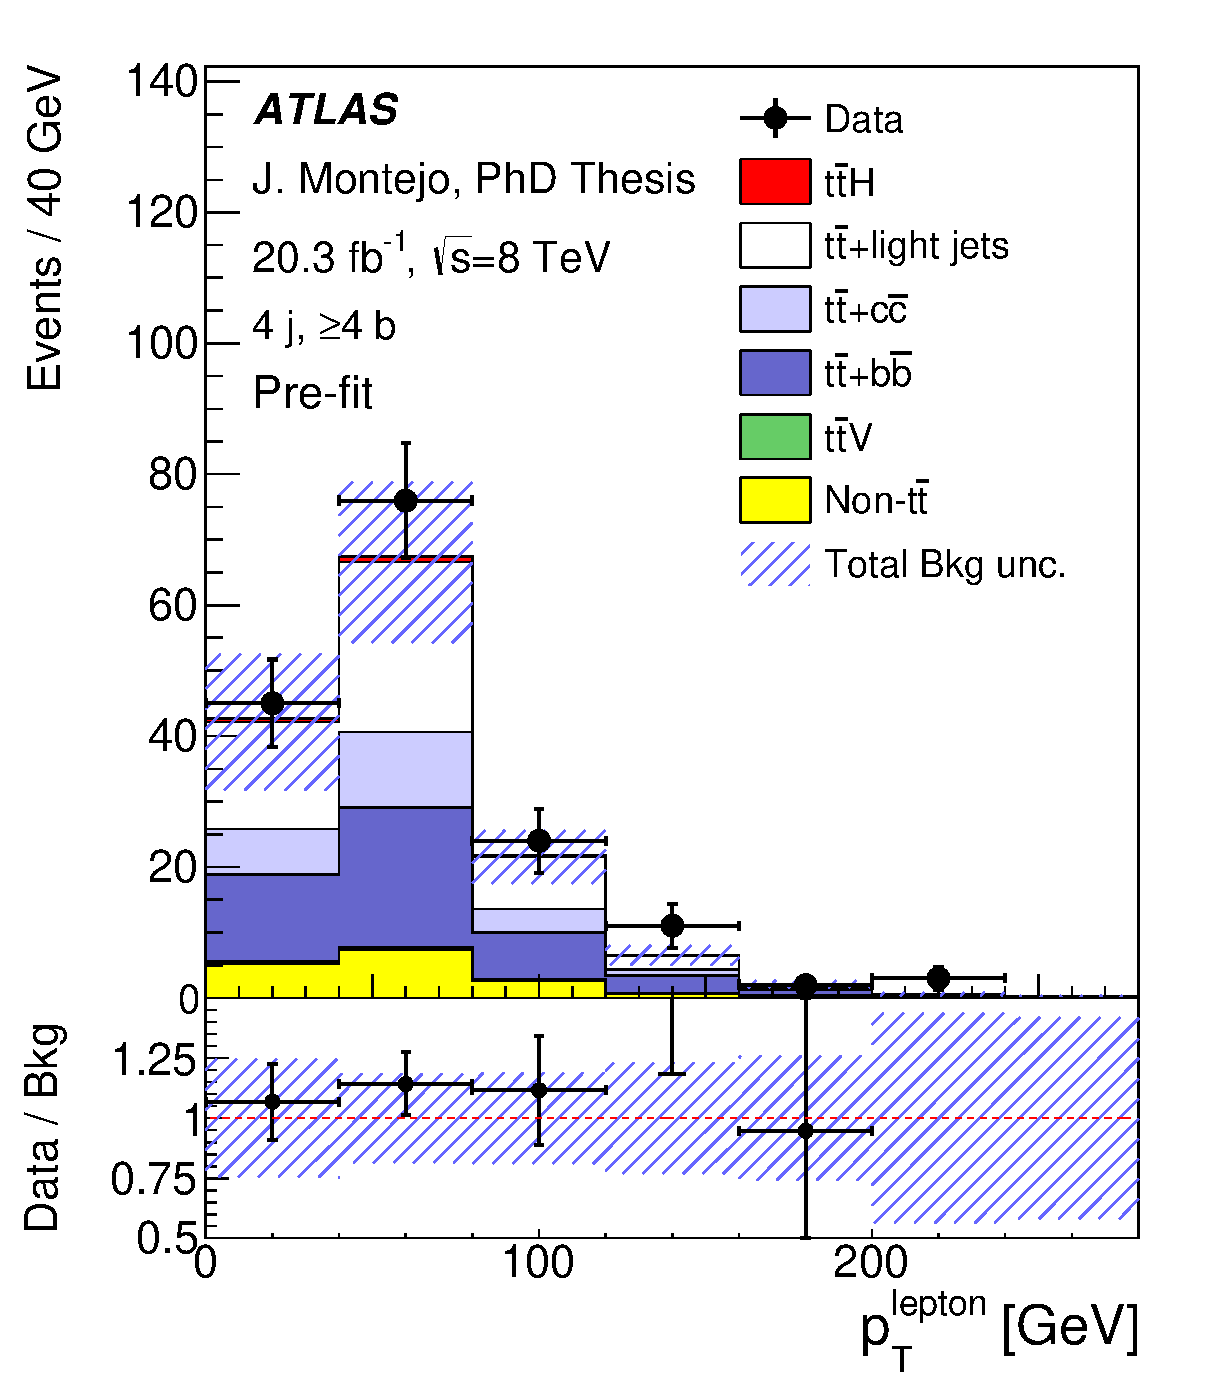
\includegraphics[width=0.27\textwidth]{Analysis/Figures_ttH/tesis_vars/prefit/lep_pt_4jetex4btagin.eps} &
  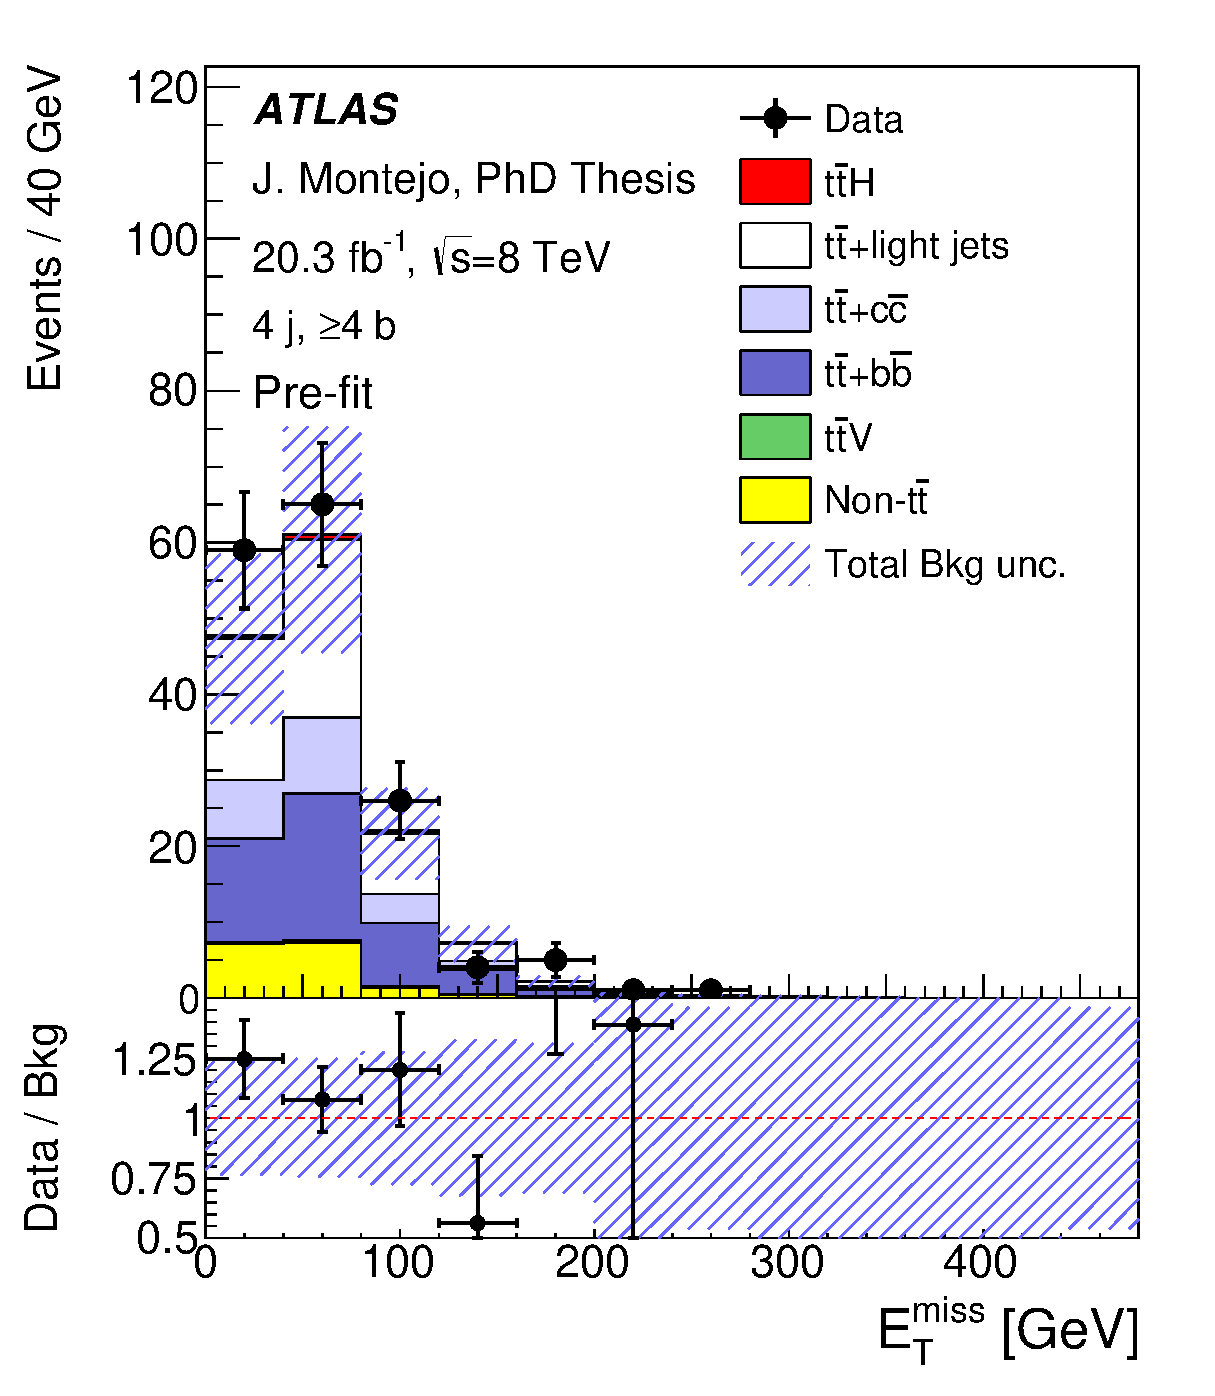
\includegraphics[width=0.27\textwidth]{Analysis/Figures_ttH/tesis_vars/prefit/met_4jetex4btagin.eps} &
  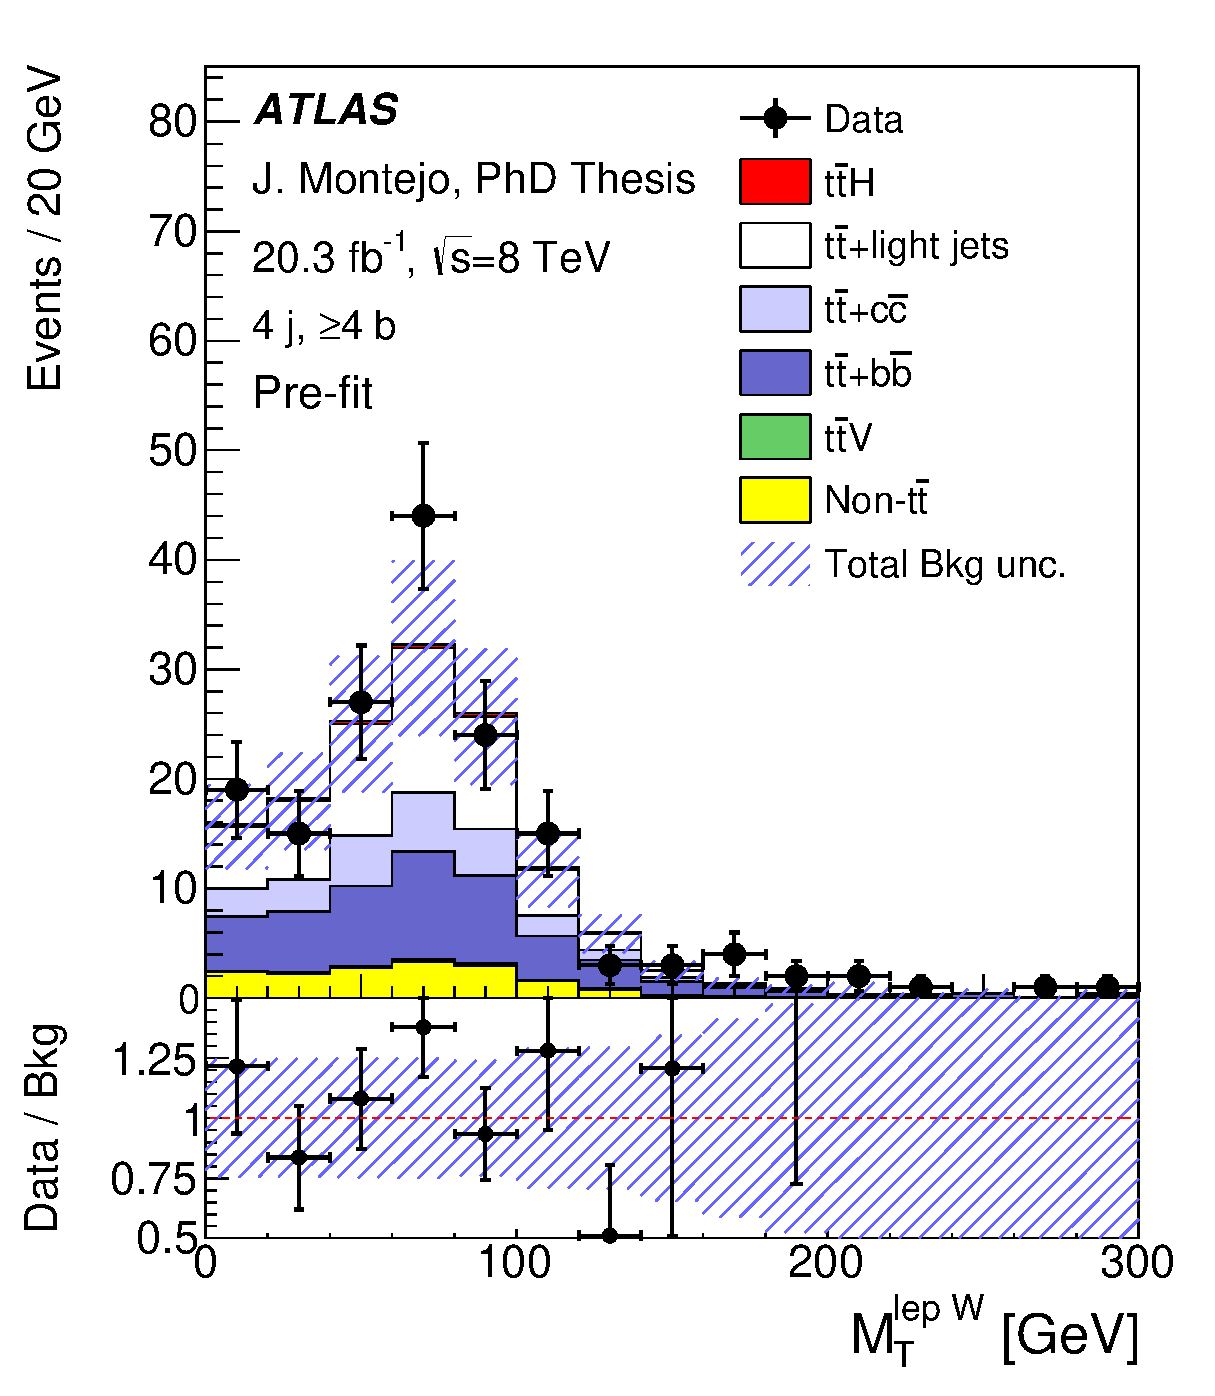
\includegraphics[width=0.27\textwidth]{Analysis/Figures_ttH/tesis_vars/prefit/WlepMT_4jetex4btagin.eps} \\
  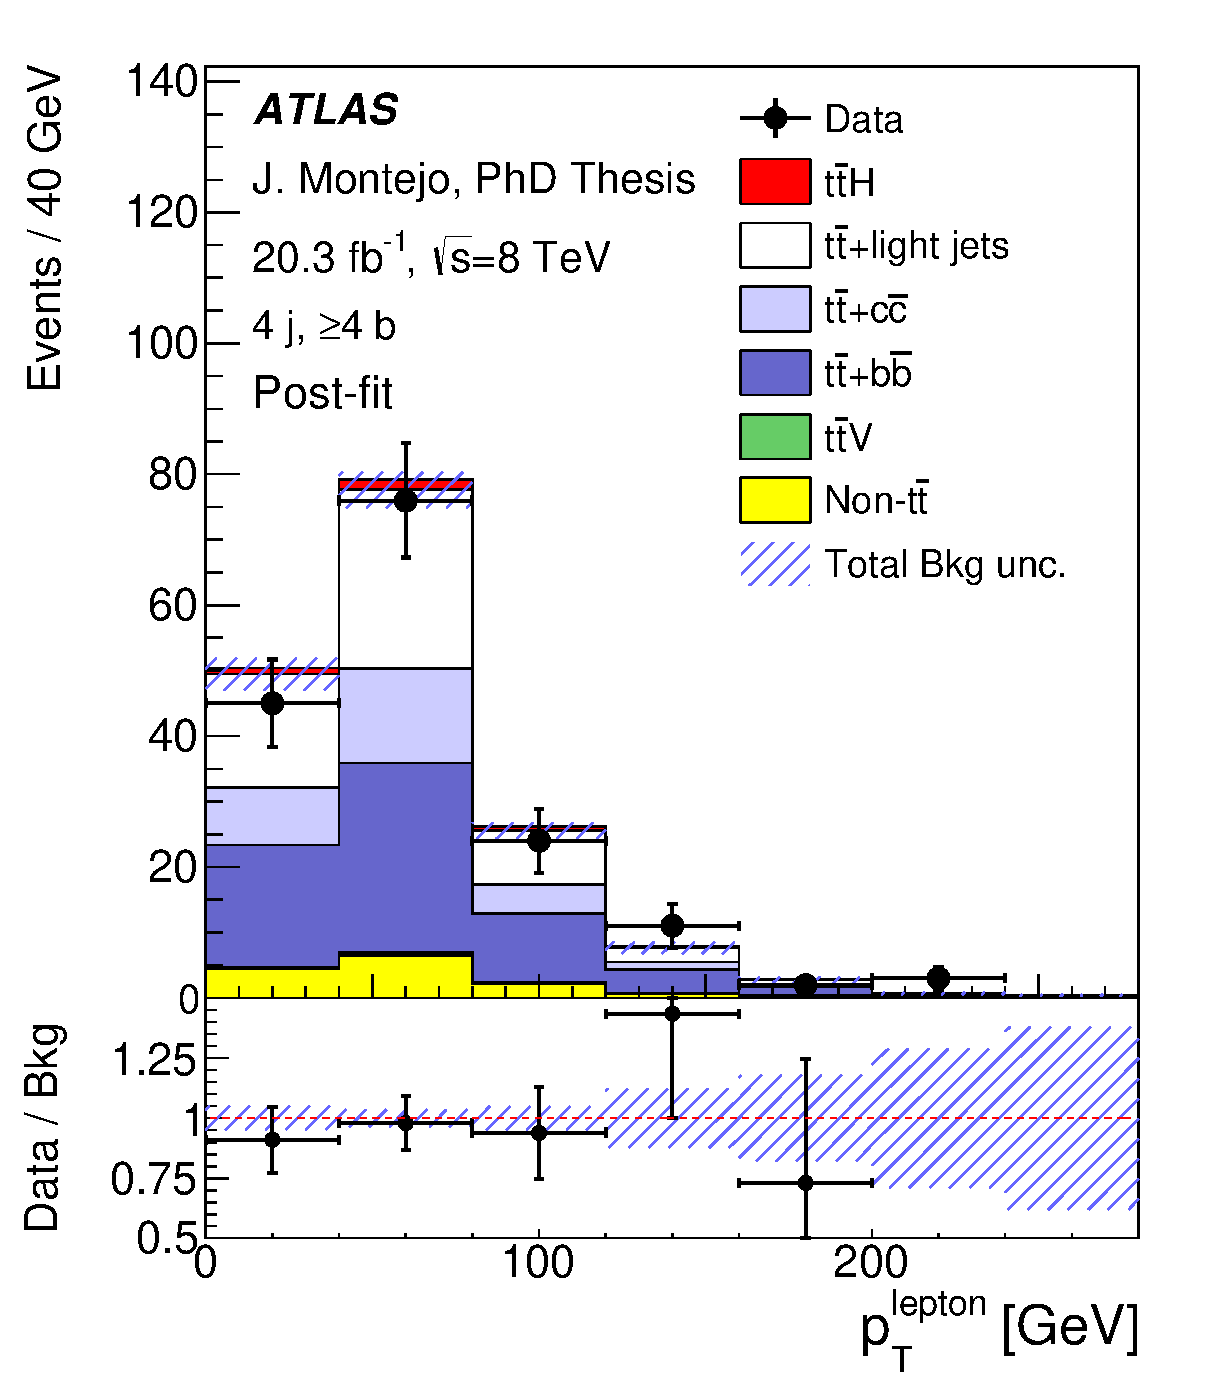
\includegraphics[width=0.27\textwidth]{Analysis/Figures_ttH/tesis_vars/postfit/lep_pt_4jetex4btagin.eps} &
  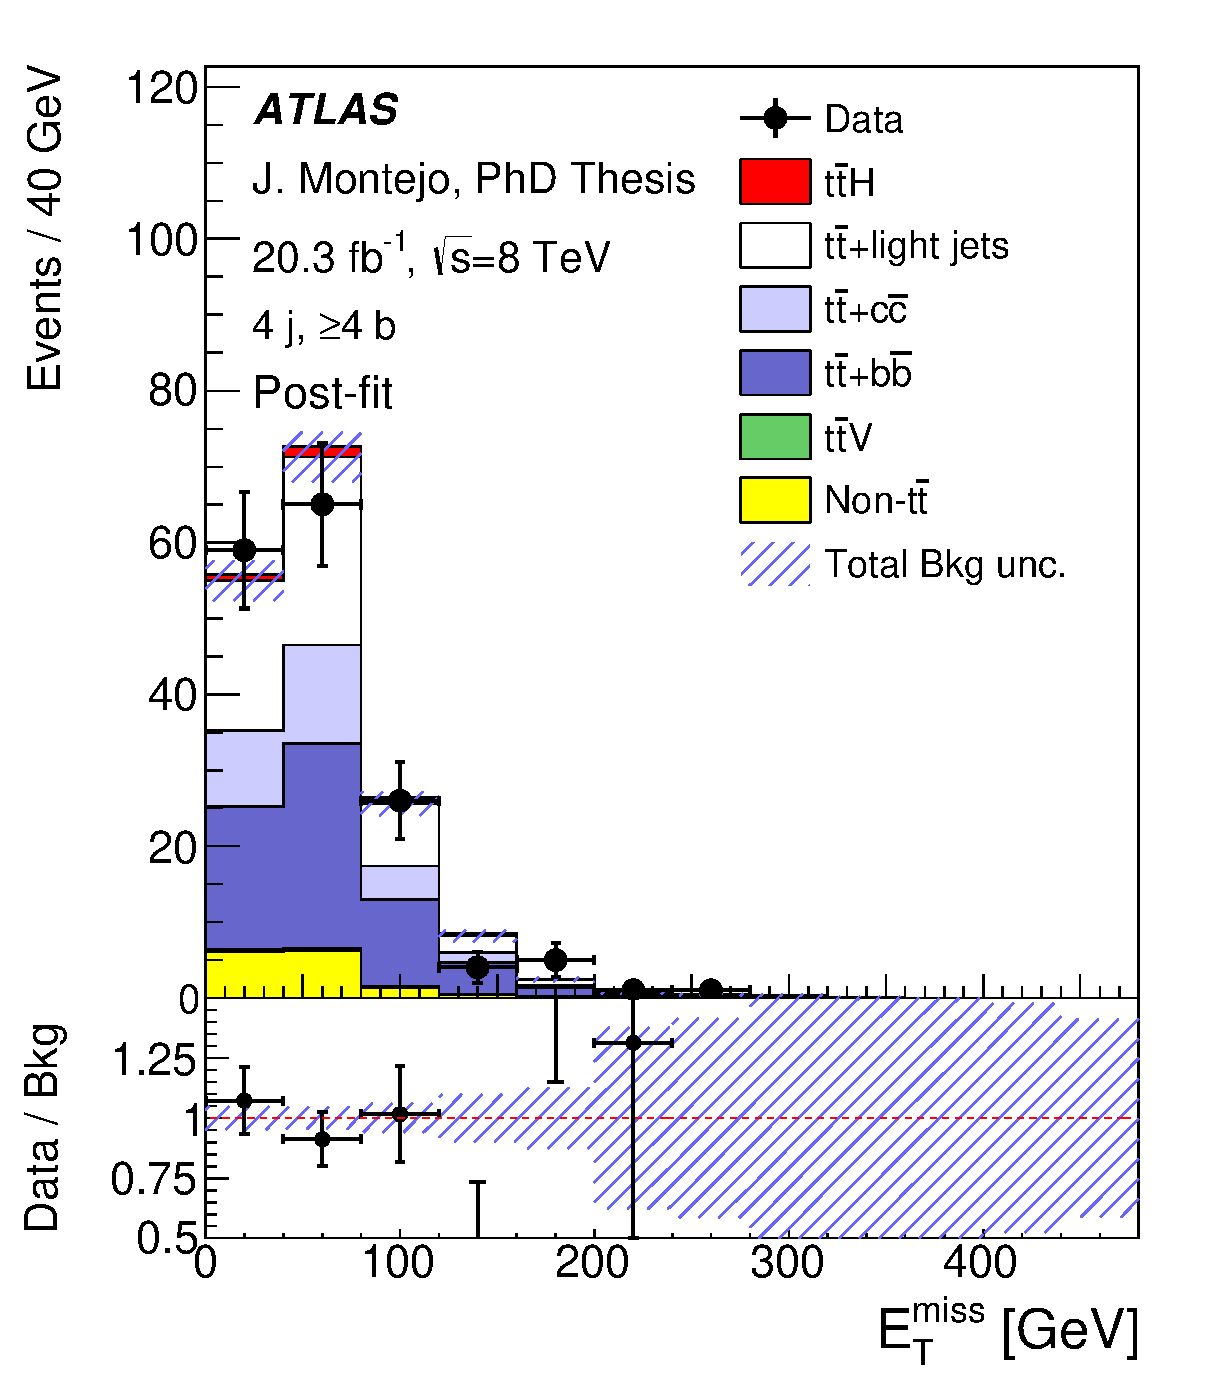
\includegraphics[width=0.27\textwidth]{Analysis/Figures_ttH/tesis_vars/postfit/met_4jetex4btagin.eps} &
  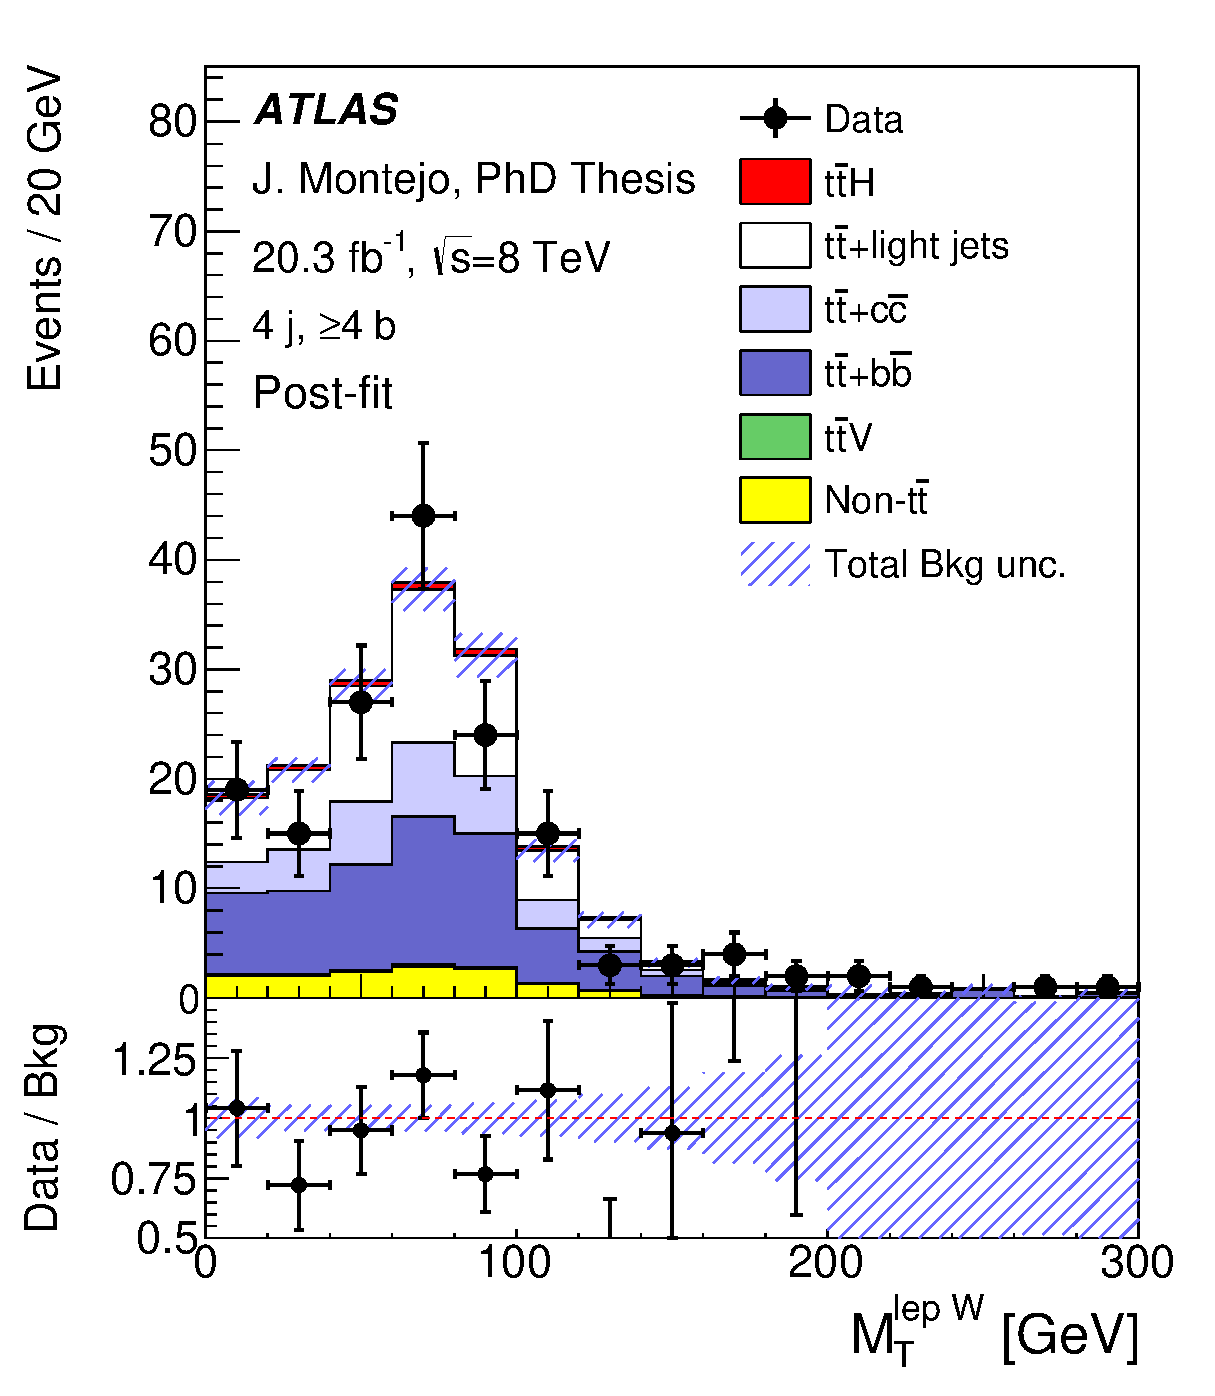
\includegraphics[width=0.27\textwidth]{Analysis/Figures_ttH/tesis_vars/postfit/WlepMT_4jetex4btagin.eps} \\
\end{tabular}
\caption{Comparison between data and prediction in the \fourfour\ region for (left) lepton \pt,  (middle) missing transverse energy, \met, and (right)  $W$ boson transverse mass, \mtw. The background prediction is shown (top) before the fit and (bottom) after the fit.}
  \label{fig:vars1_fourfour}
\vspace{0.5cm}
  \centering
  \begin{tabular}{ccc}
  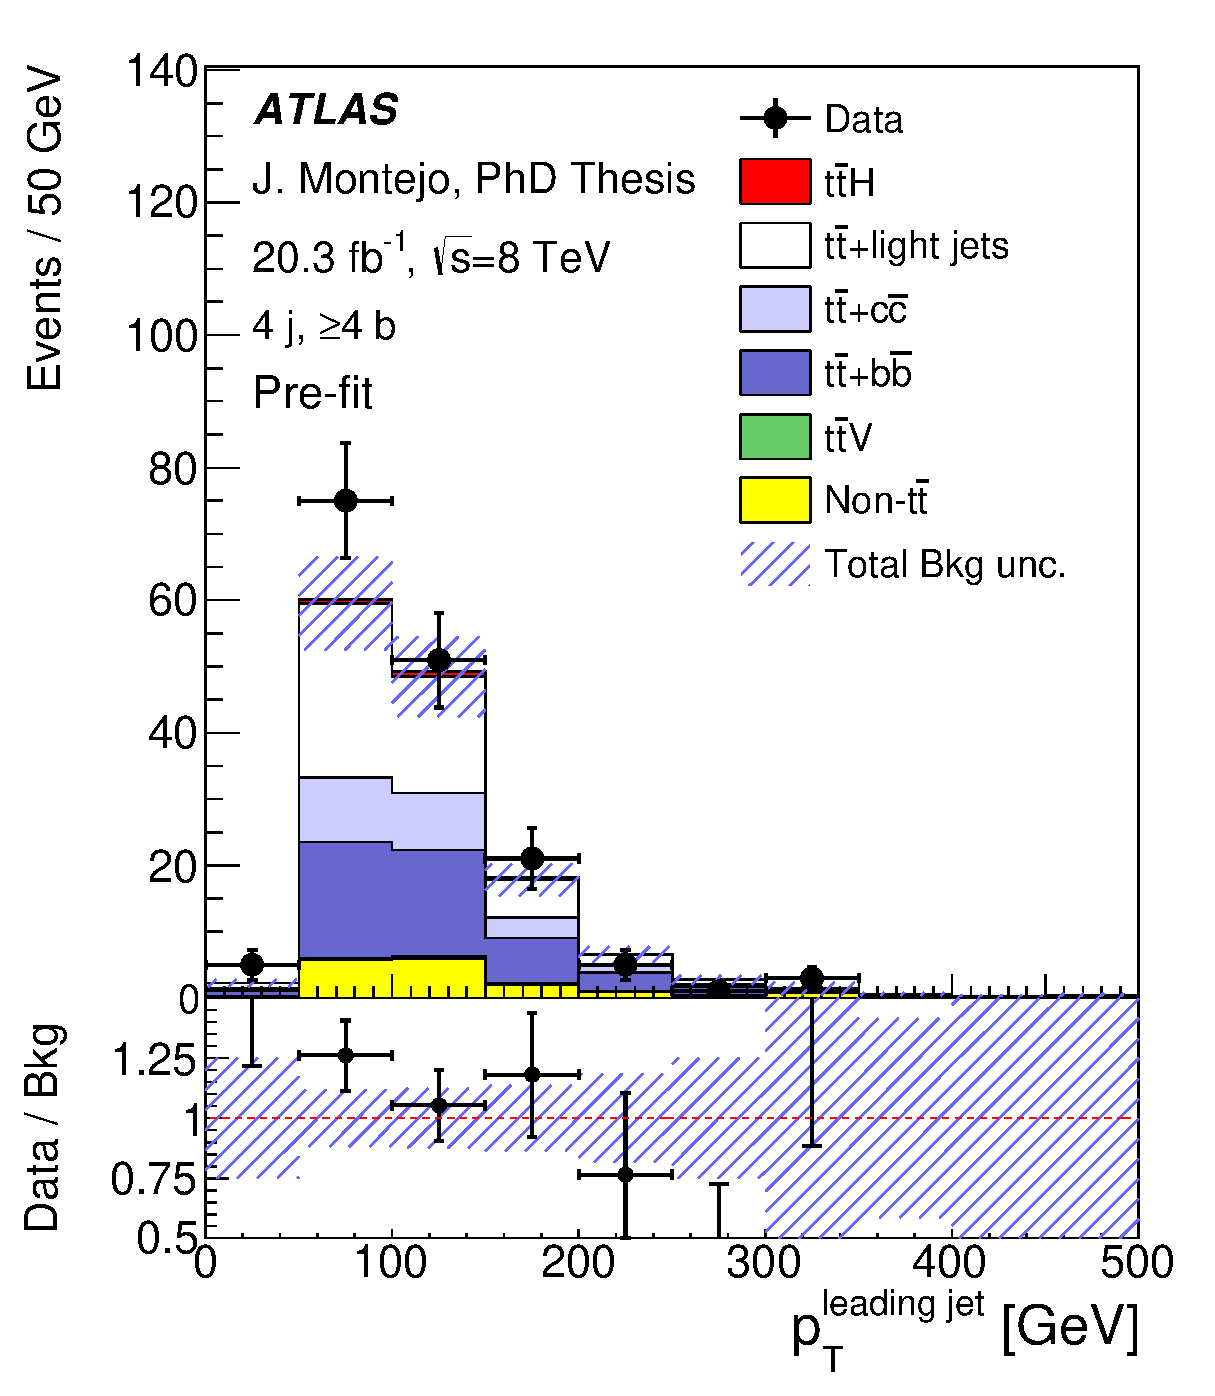
\includegraphics[width=0.27\textwidth]{Analysis/Figures_ttH/tesis_vars/prefit/jet1_pt_4jetex4btagin.eps} &
  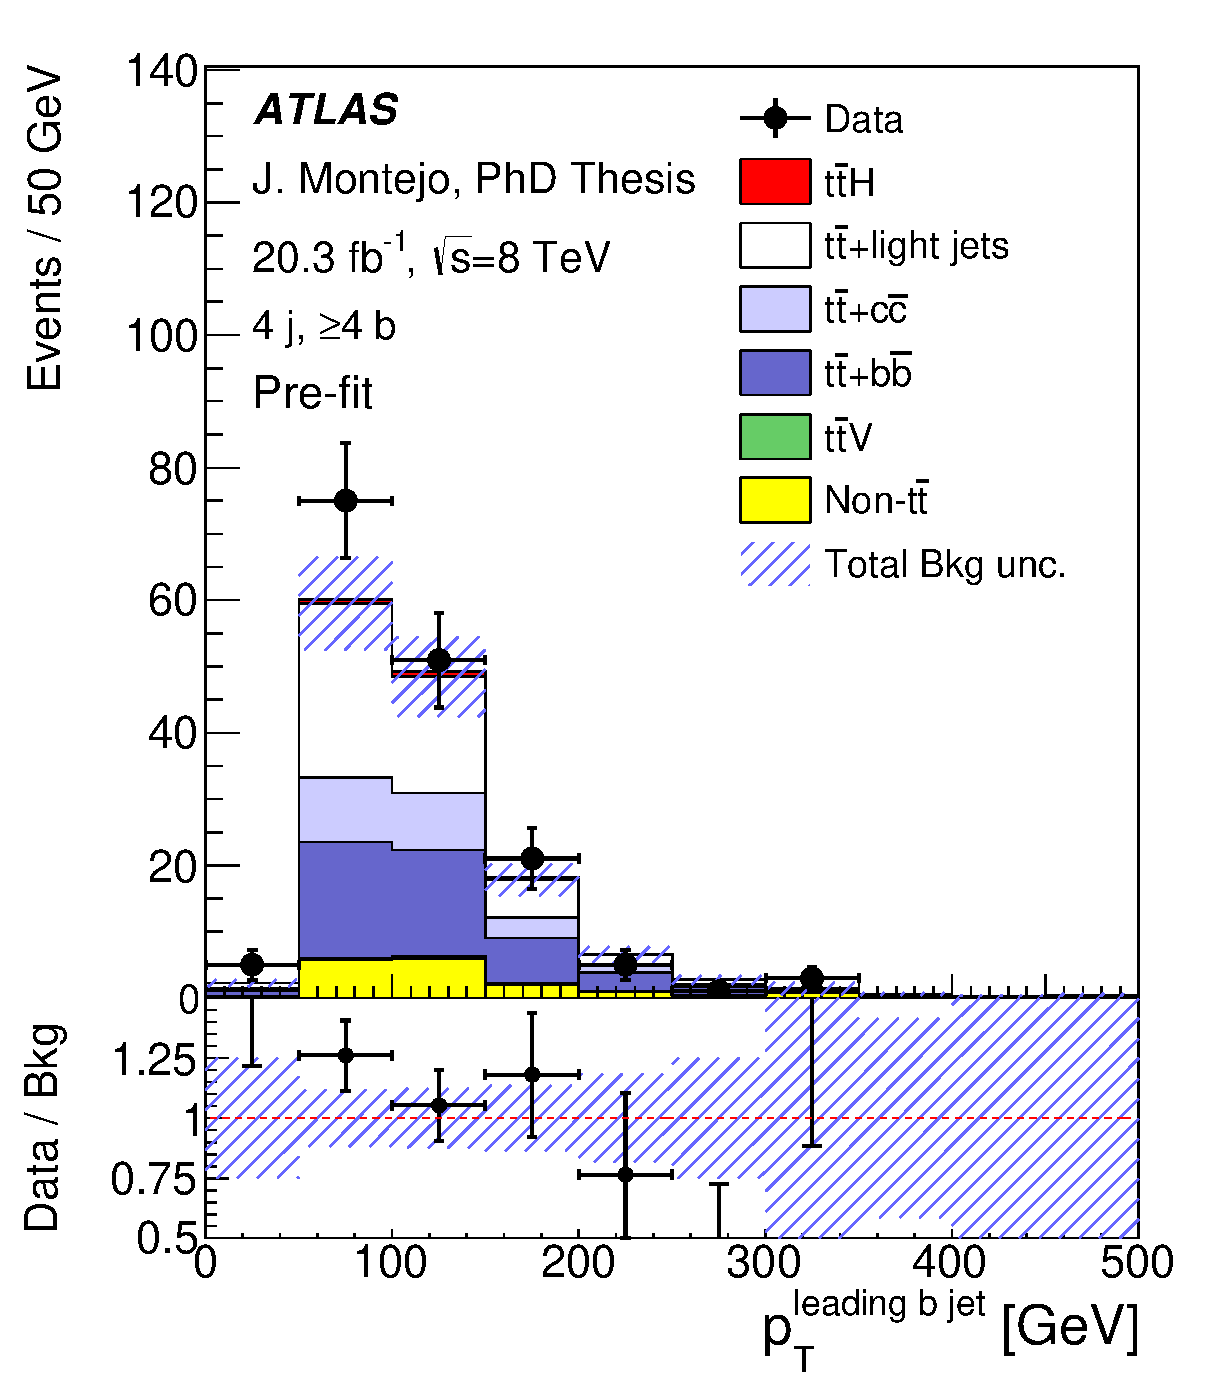
\includegraphics[width=0.27\textwidth]{Analysis/Figures_ttH/tesis_vars/prefit/bjet1_pt_4jetex4btagin.eps} &
  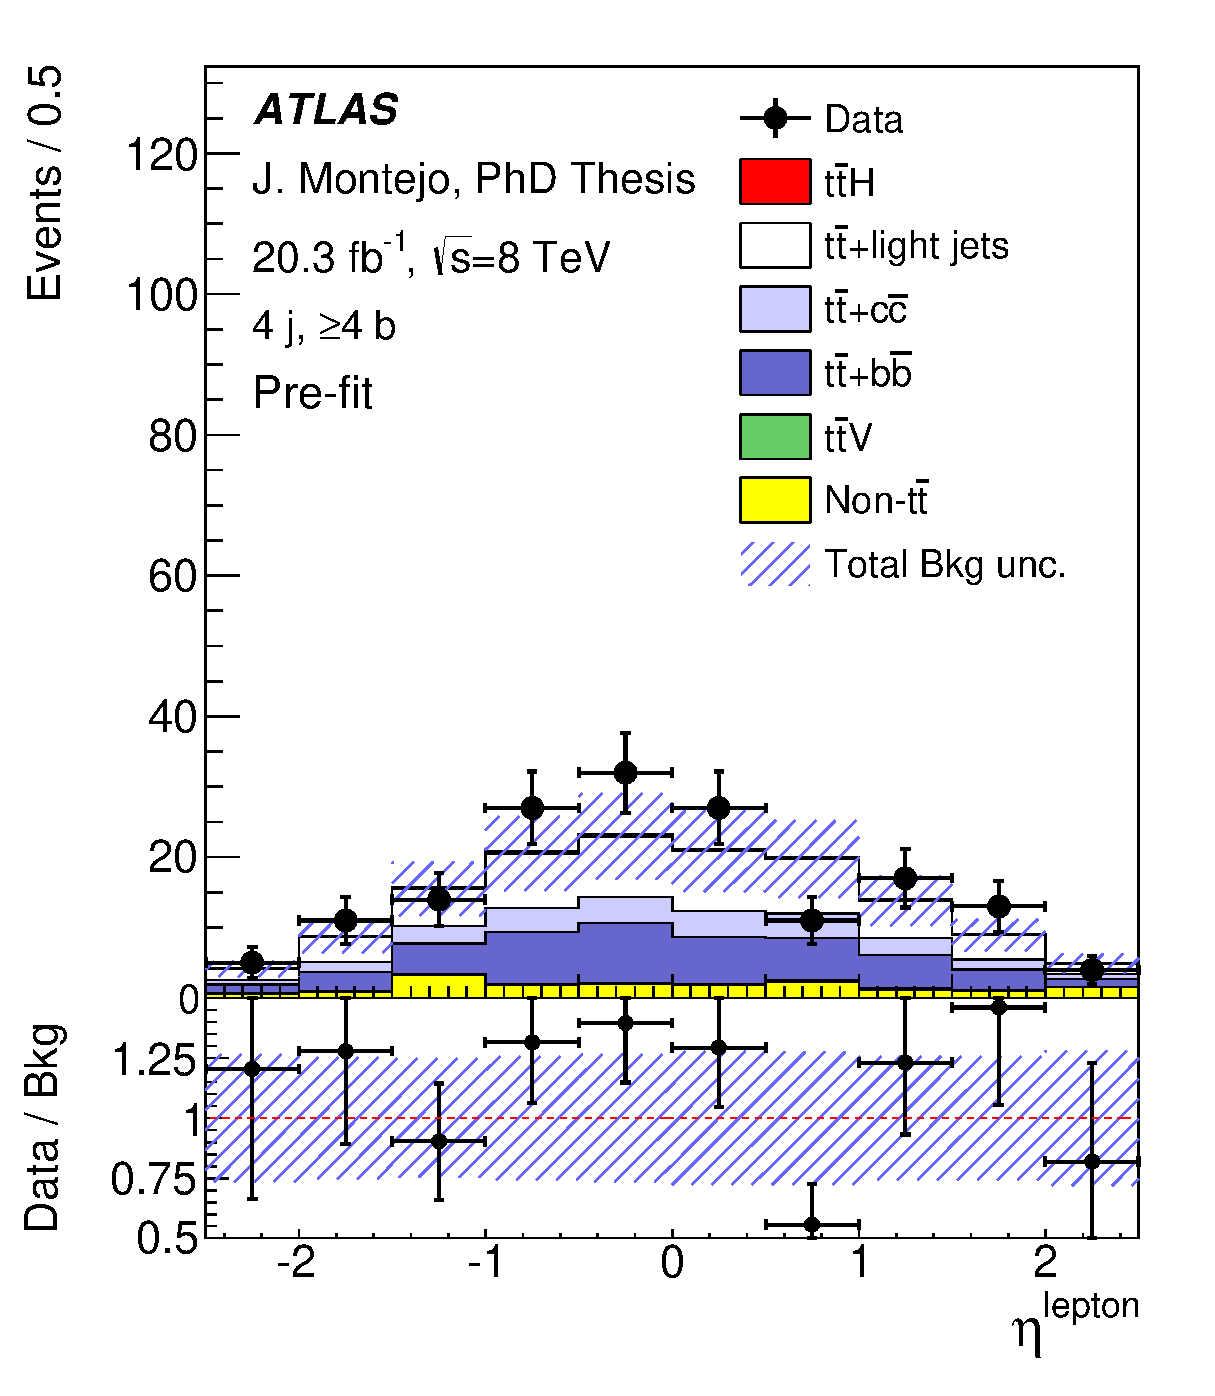
\includegraphics[width=0.27\textwidth]{Analysis/Figures_ttH/tesis_vars/prefit/lep_eta_4jetex4btagin.eps} \\
  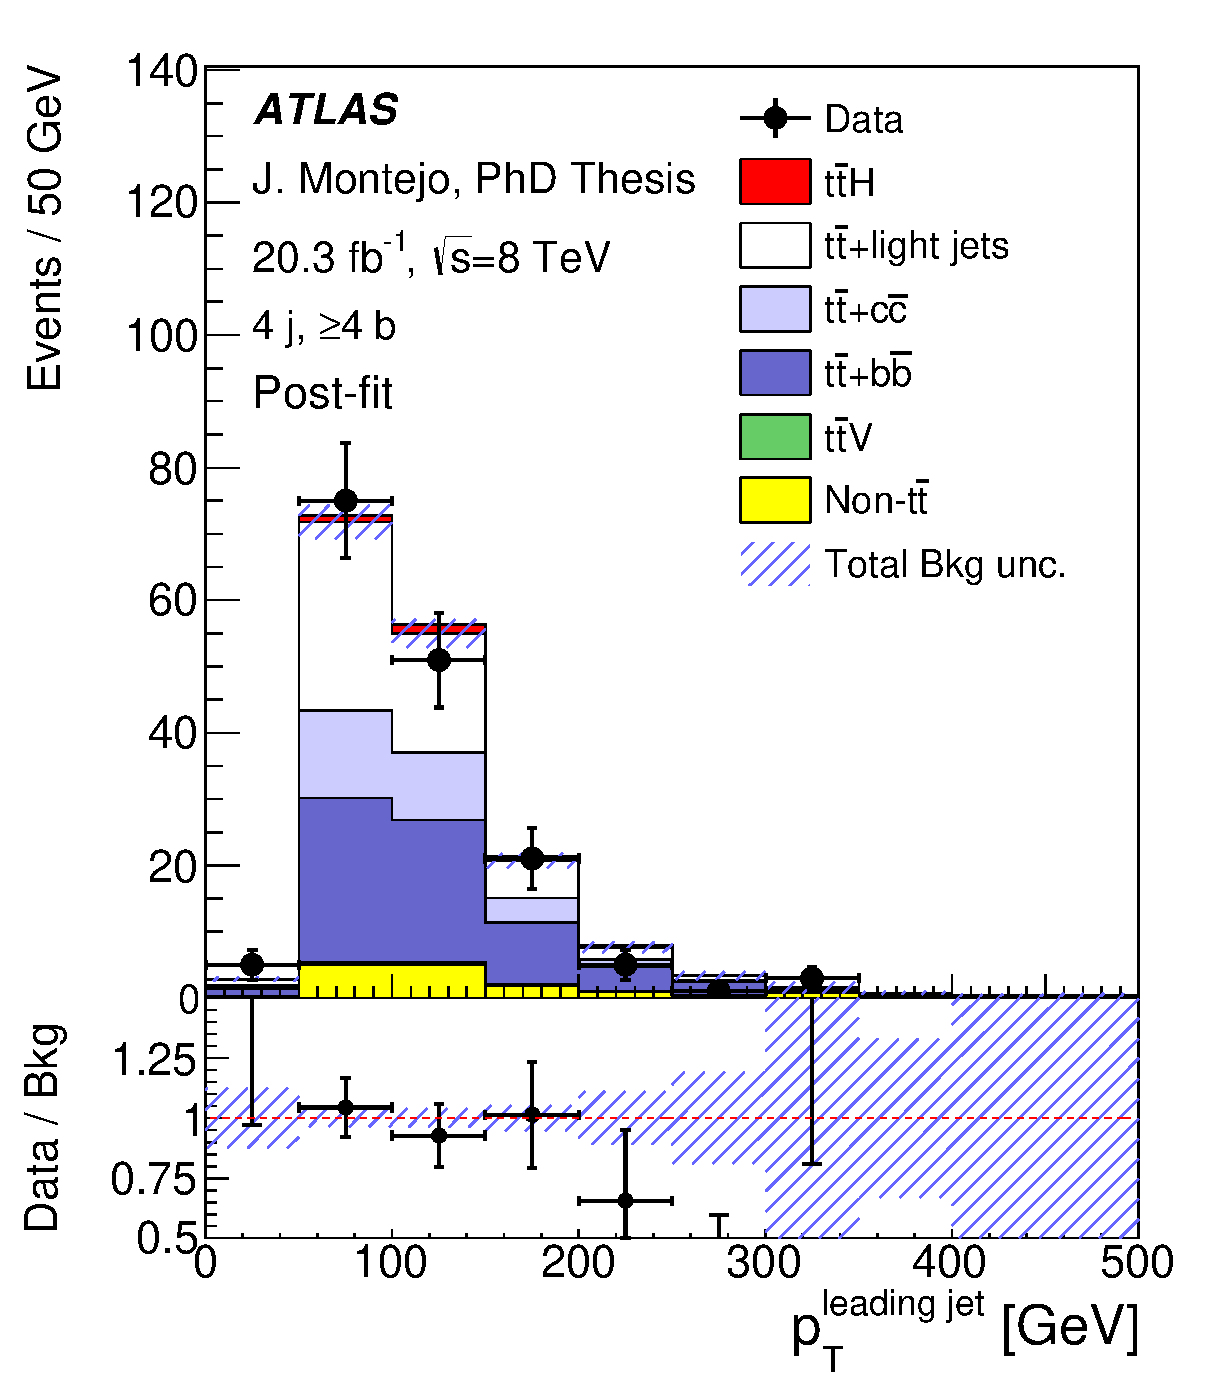
\includegraphics[width=0.27\textwidth]{Analysis/Figures_ttH/tesis_vars/postfit/jet1_pt_4jetex4btagin.eps} &
  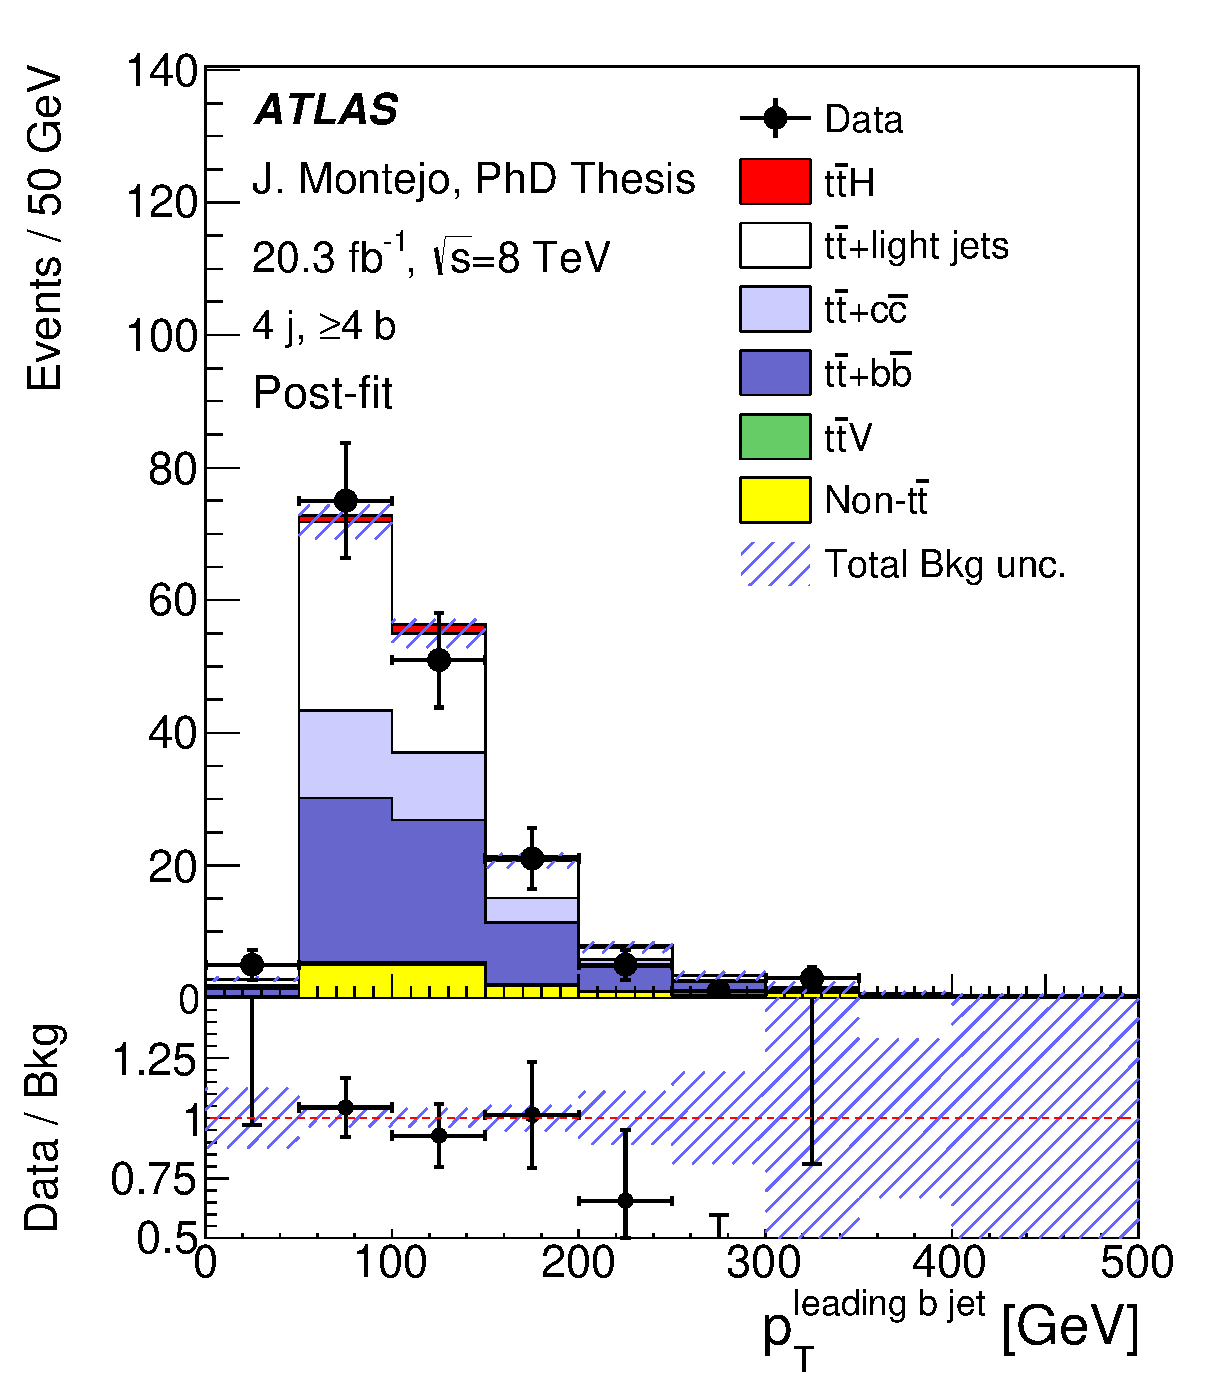
\includegraphics[width=0.27\textwidth]{Analysis/Figures_ttH/tesis_vars/postfit/bjet1_pt_4jetex4btagin.eps} &
  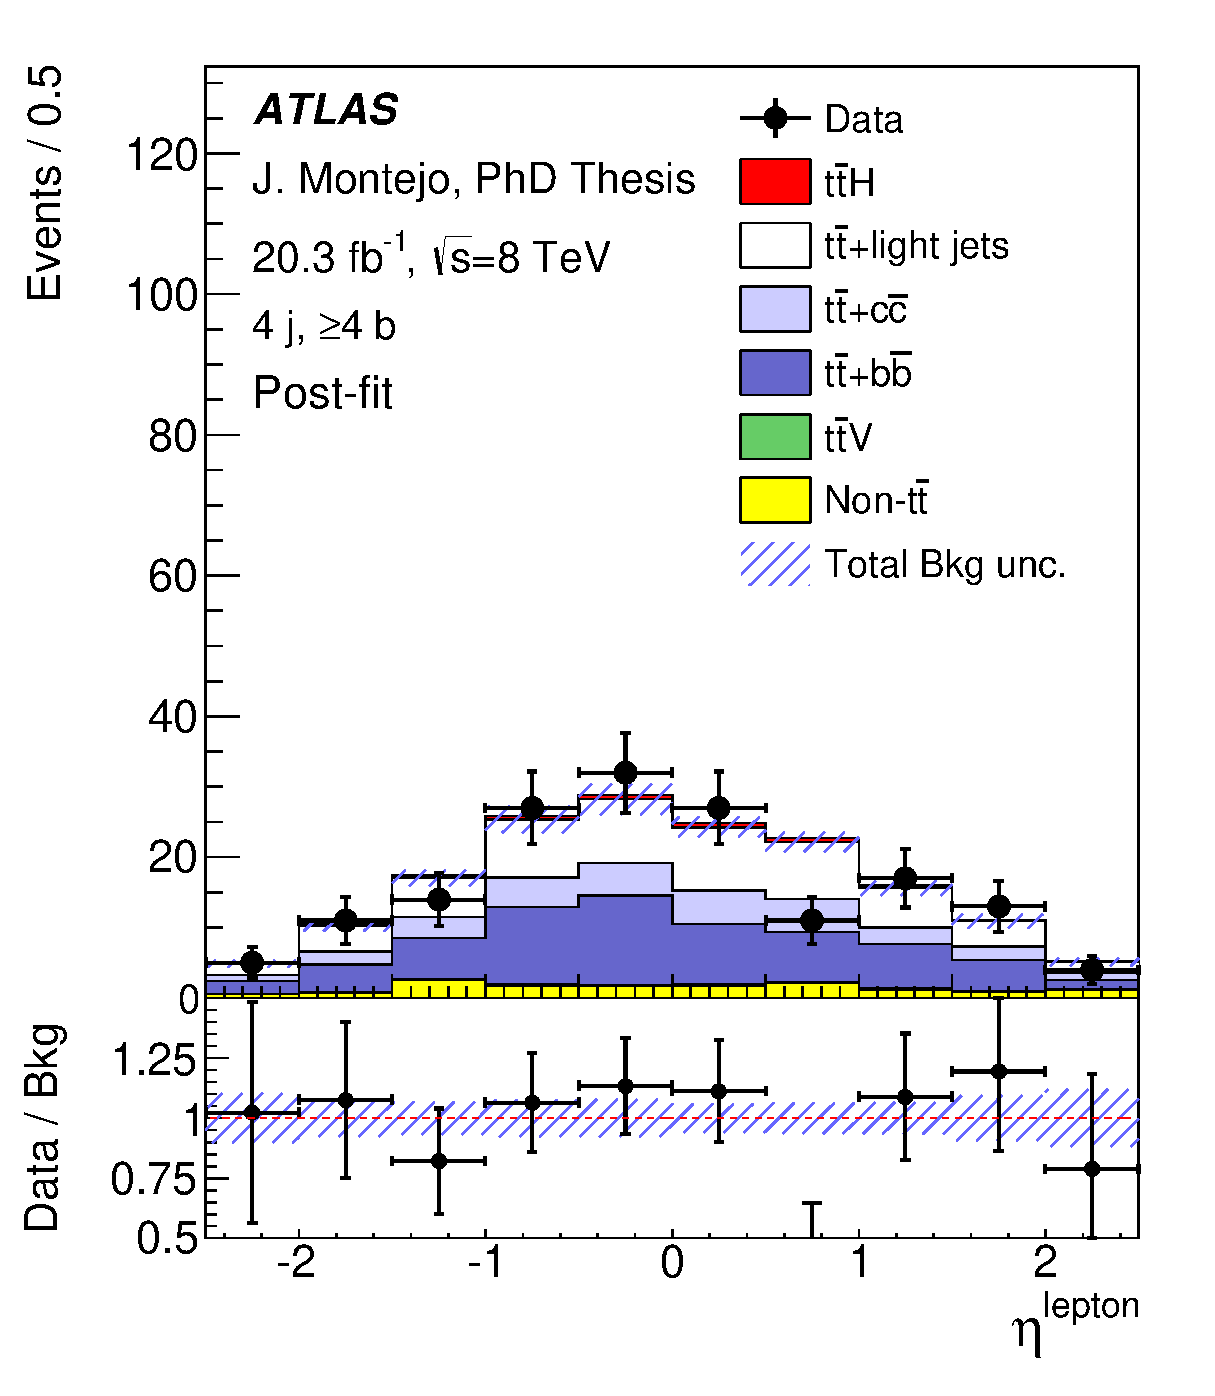
\includegraphics[width=0.27\textwidth]{Analysis/Figures_ttH/tesis_vars/postfit/lep_eta_4jetex4btagin.eps} \\
\end{tabular}
\caption{Comparison between data and prediction in the \fourfour\ region for (left) leading jet \pt, (middle) leading $b$-tagged jet \pt, (right) lepton pseudo-rapidity. The background prediction is shown (top) before the fit and (bottom) after the fit.}
  \label{fig:vars2_fourfour}
\end{figure}
\begin{figure}[tp]
  \centering
  \begin{tabular}{ccc}
  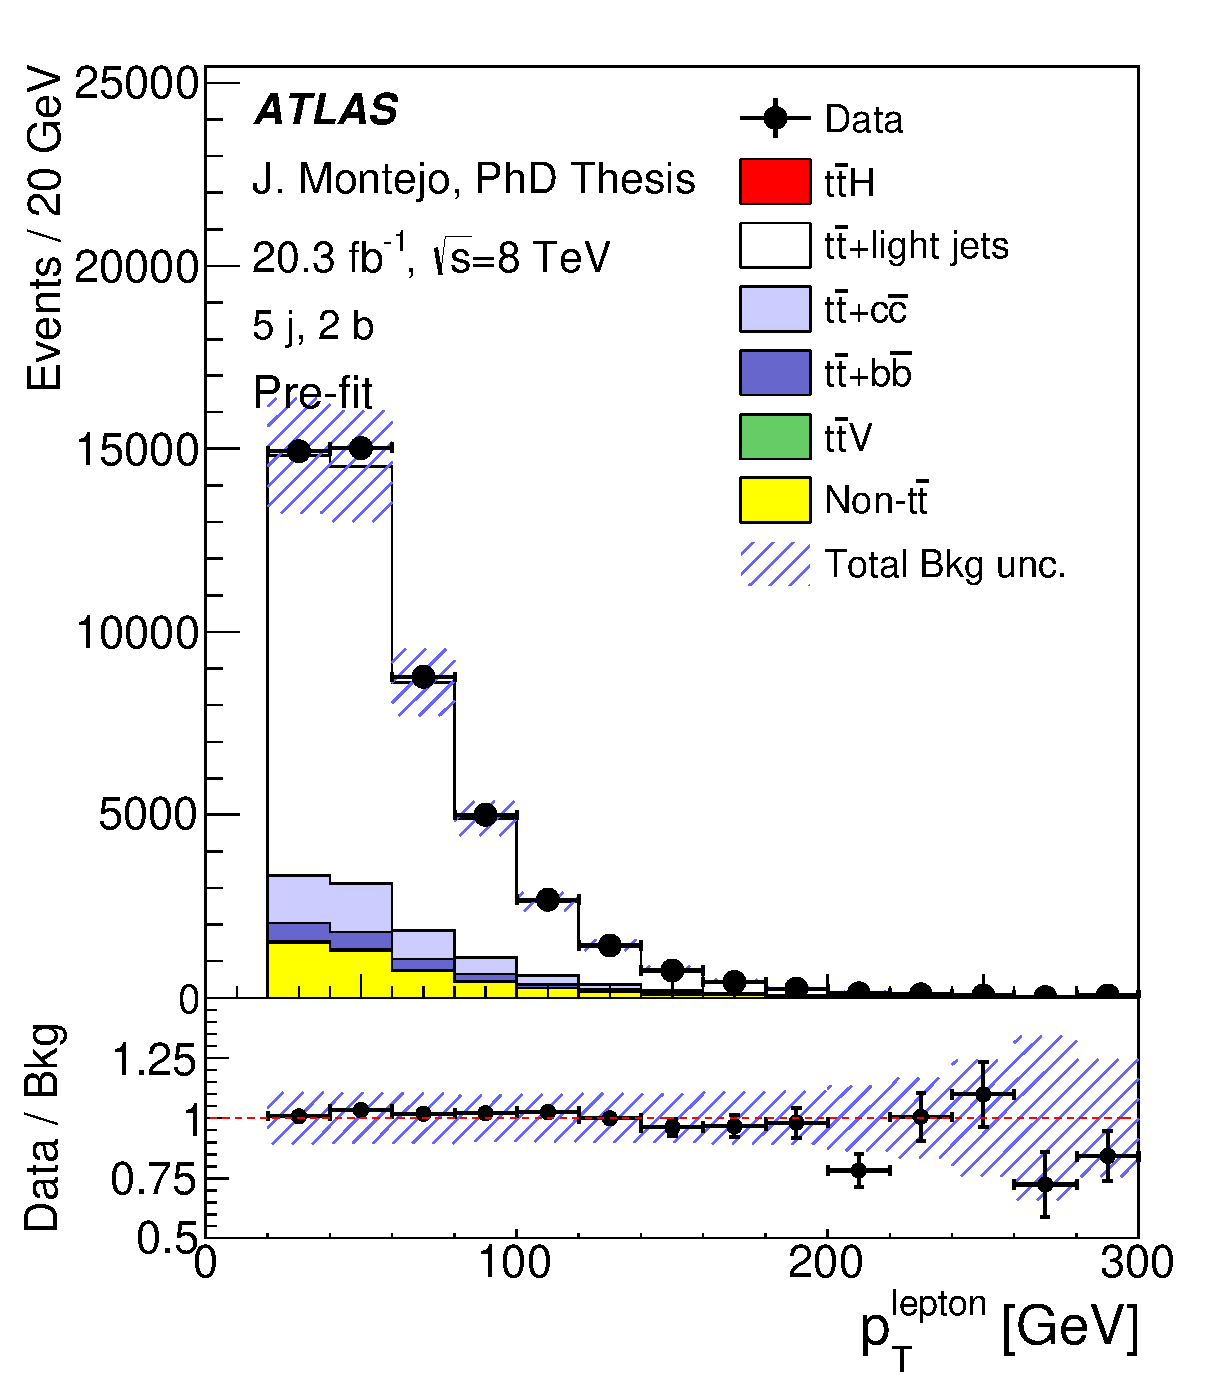
\includegraphics[width=0.27\textwidth]{Analysis/Figures_ttH/tesis_vars/prefit/lep_pt_5jetex2btagex.eps} &
  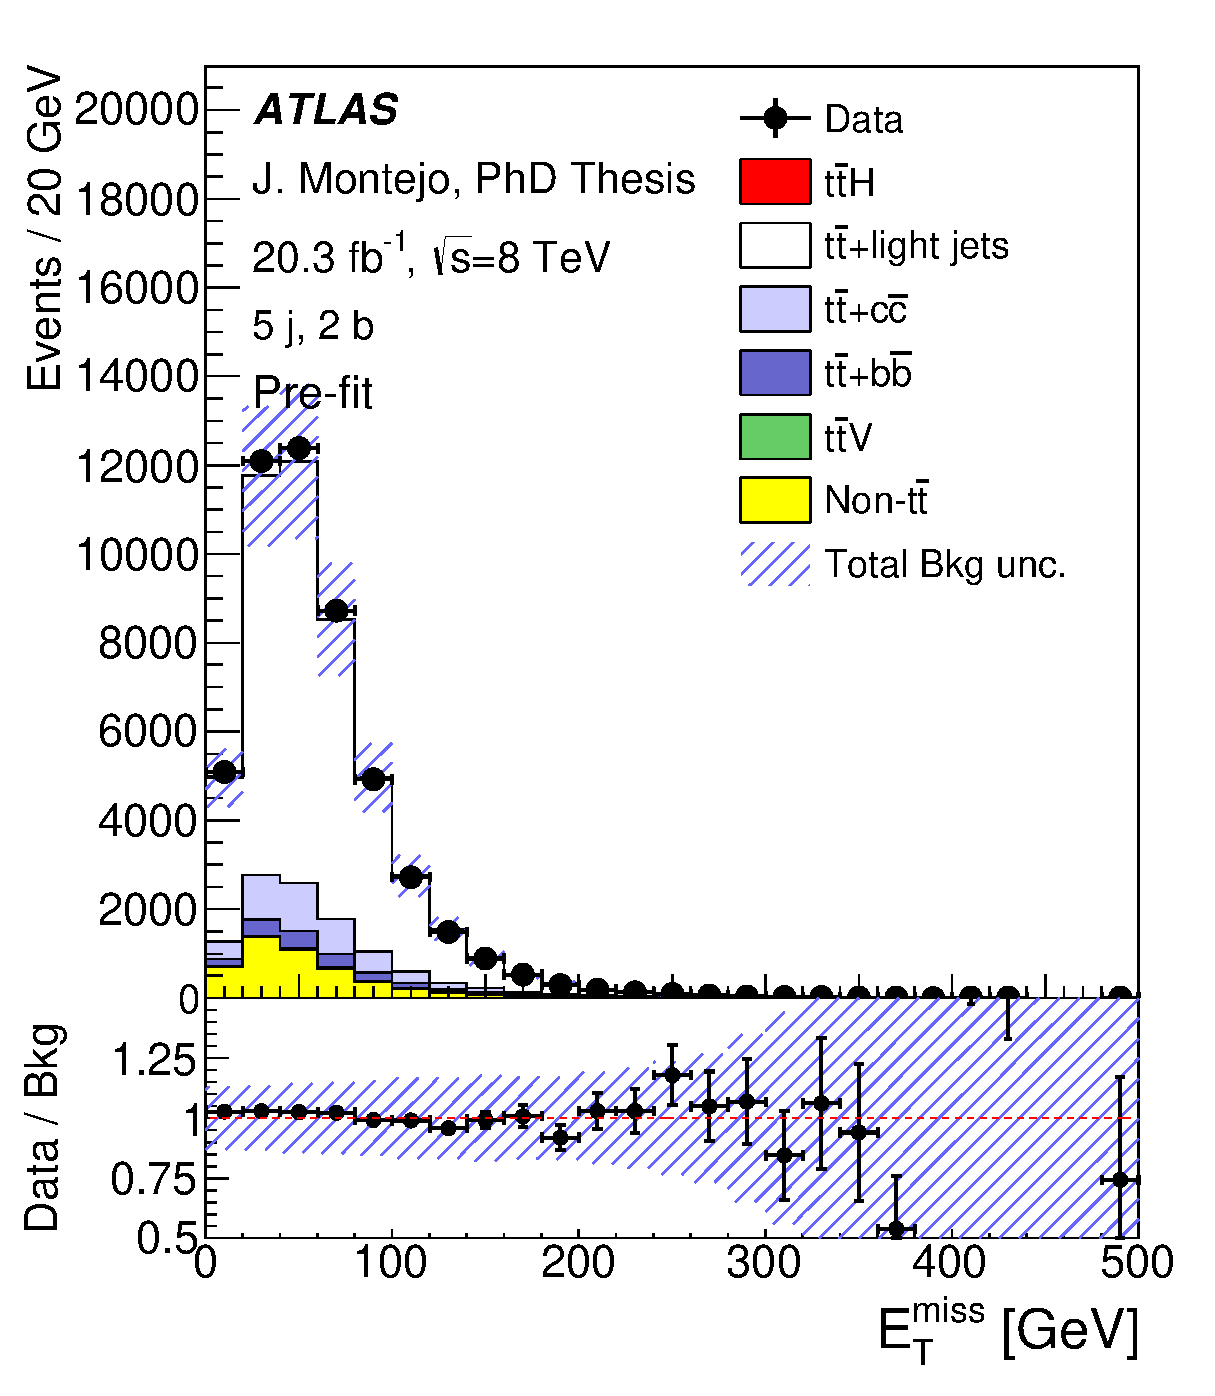
\includegraphics[width=0.27\textwidth]{Analysis/Figures_ttH/tesis_vars/prefit/met_5jetex2btagex.eps} &
  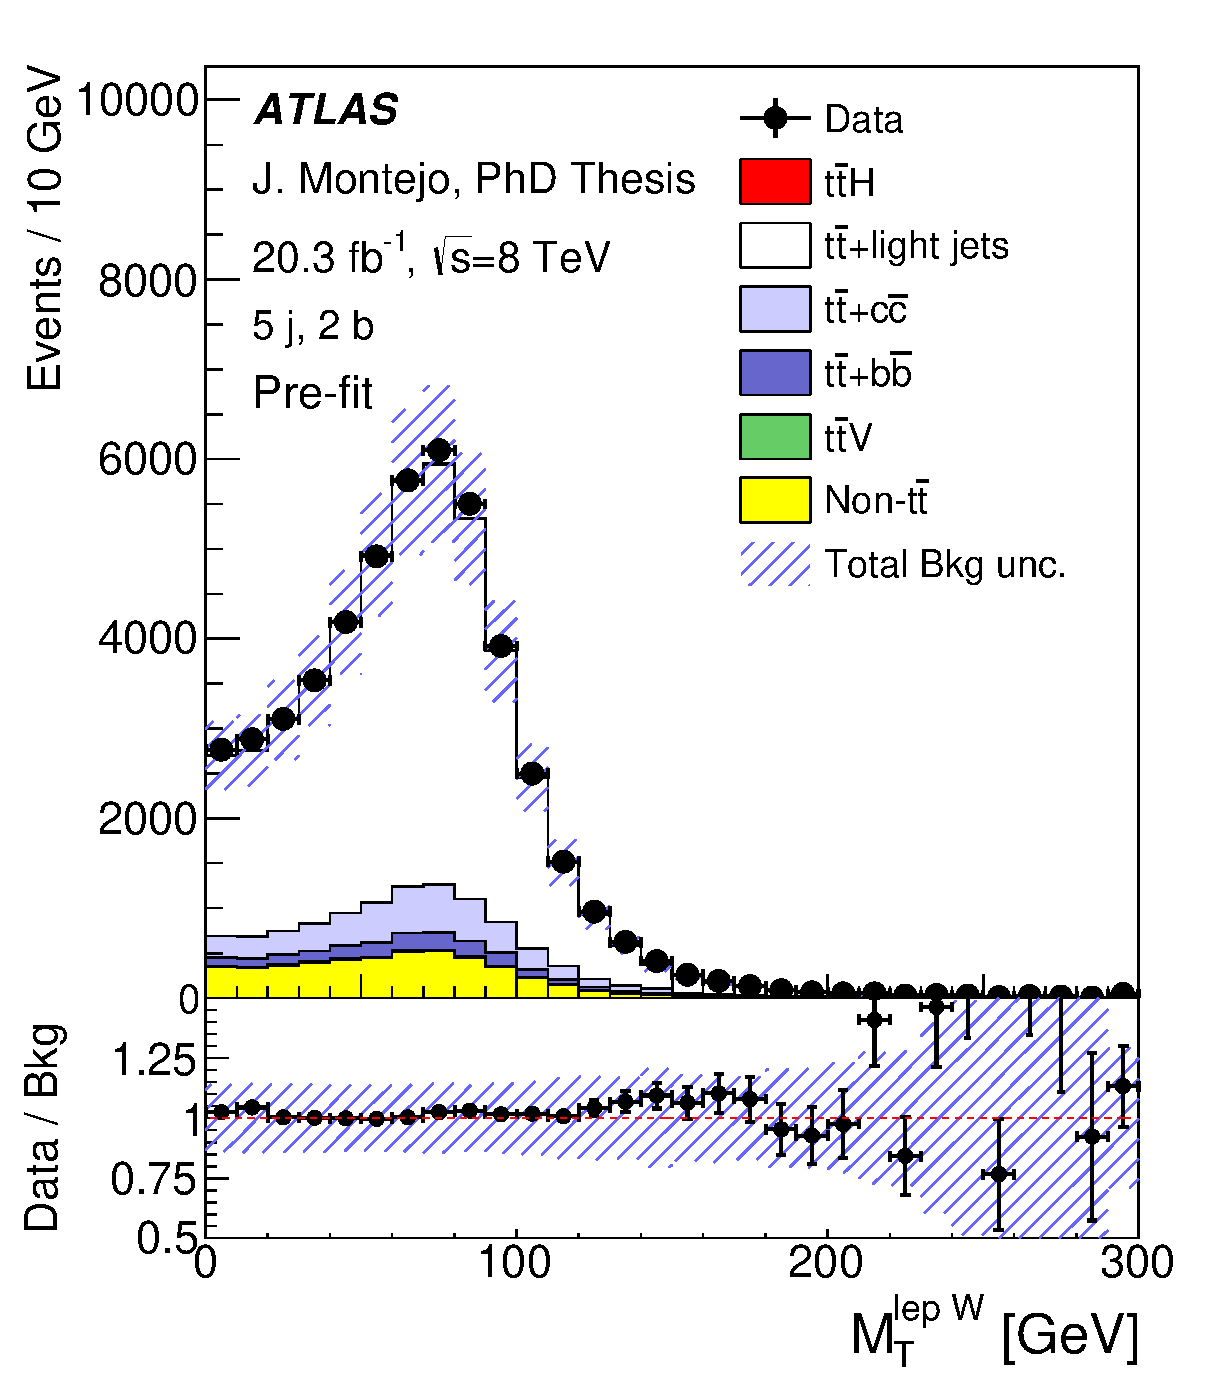
\includegraphics[width=0.27\textwidth]{Analysis/Figures_ttH/tesis_vars/prefit/WlepMT_5jetex2btagex.eps} \\
  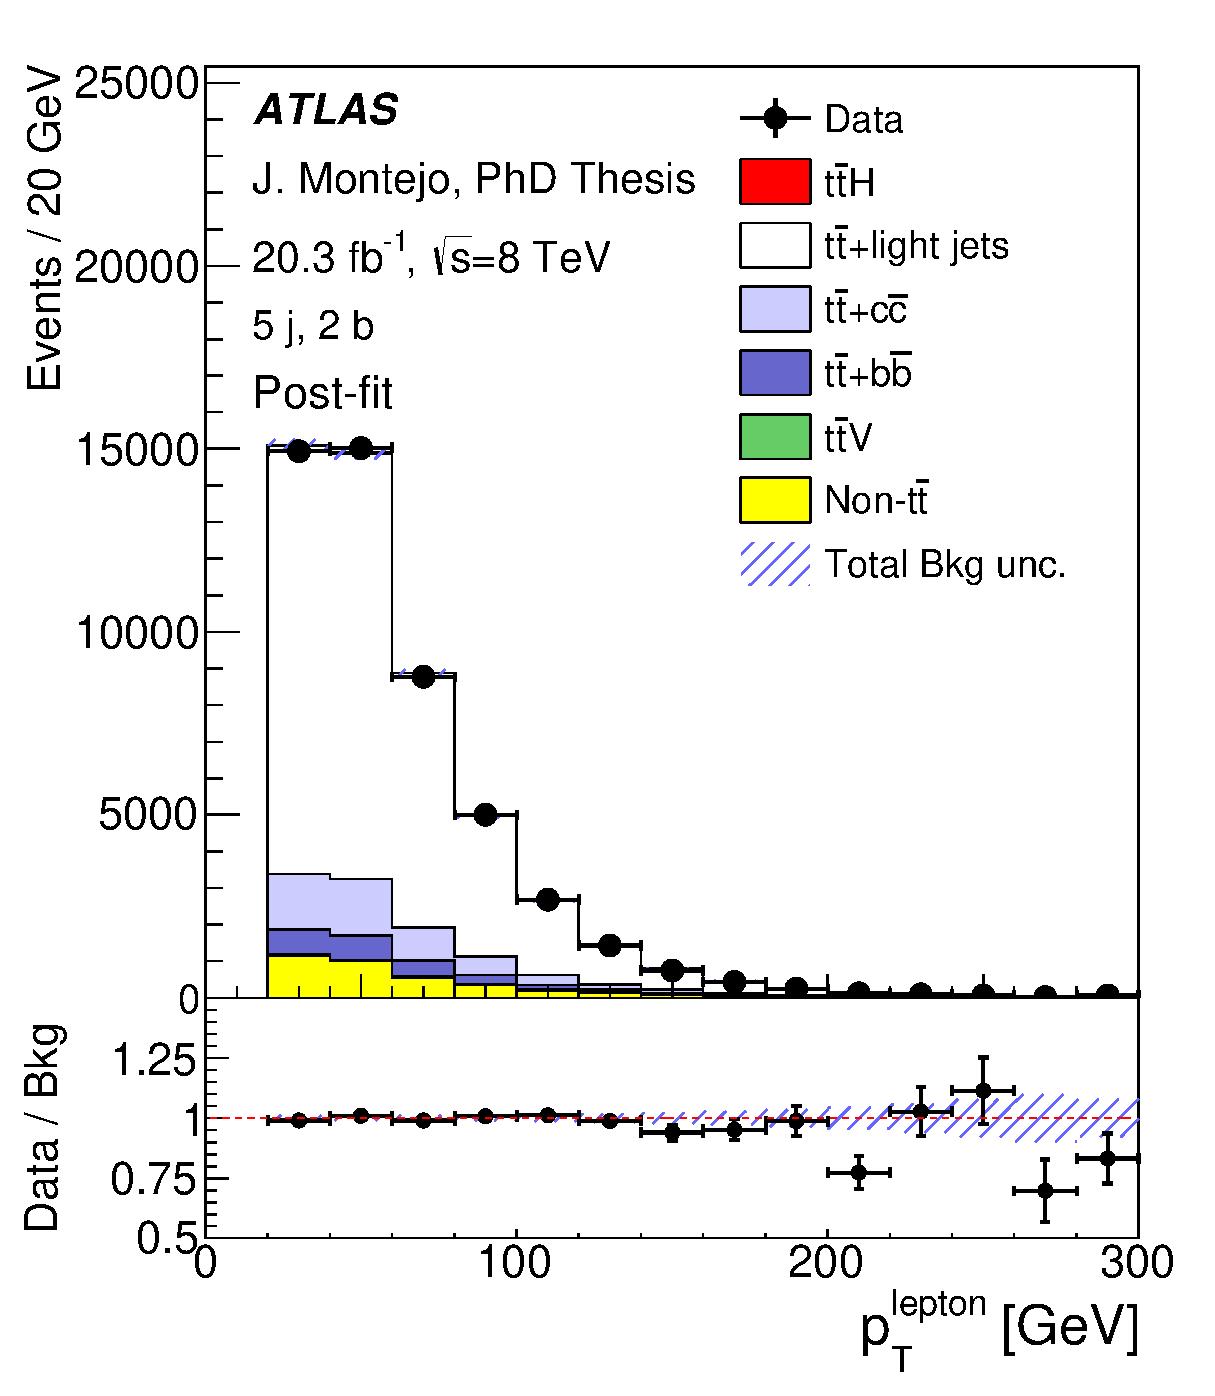
\includegraphics[width=0.27\textwidth]{Analysis/Figures_ttH/tesis_vars/postfit/lep_pt_5jetex2btagex.eps} &
  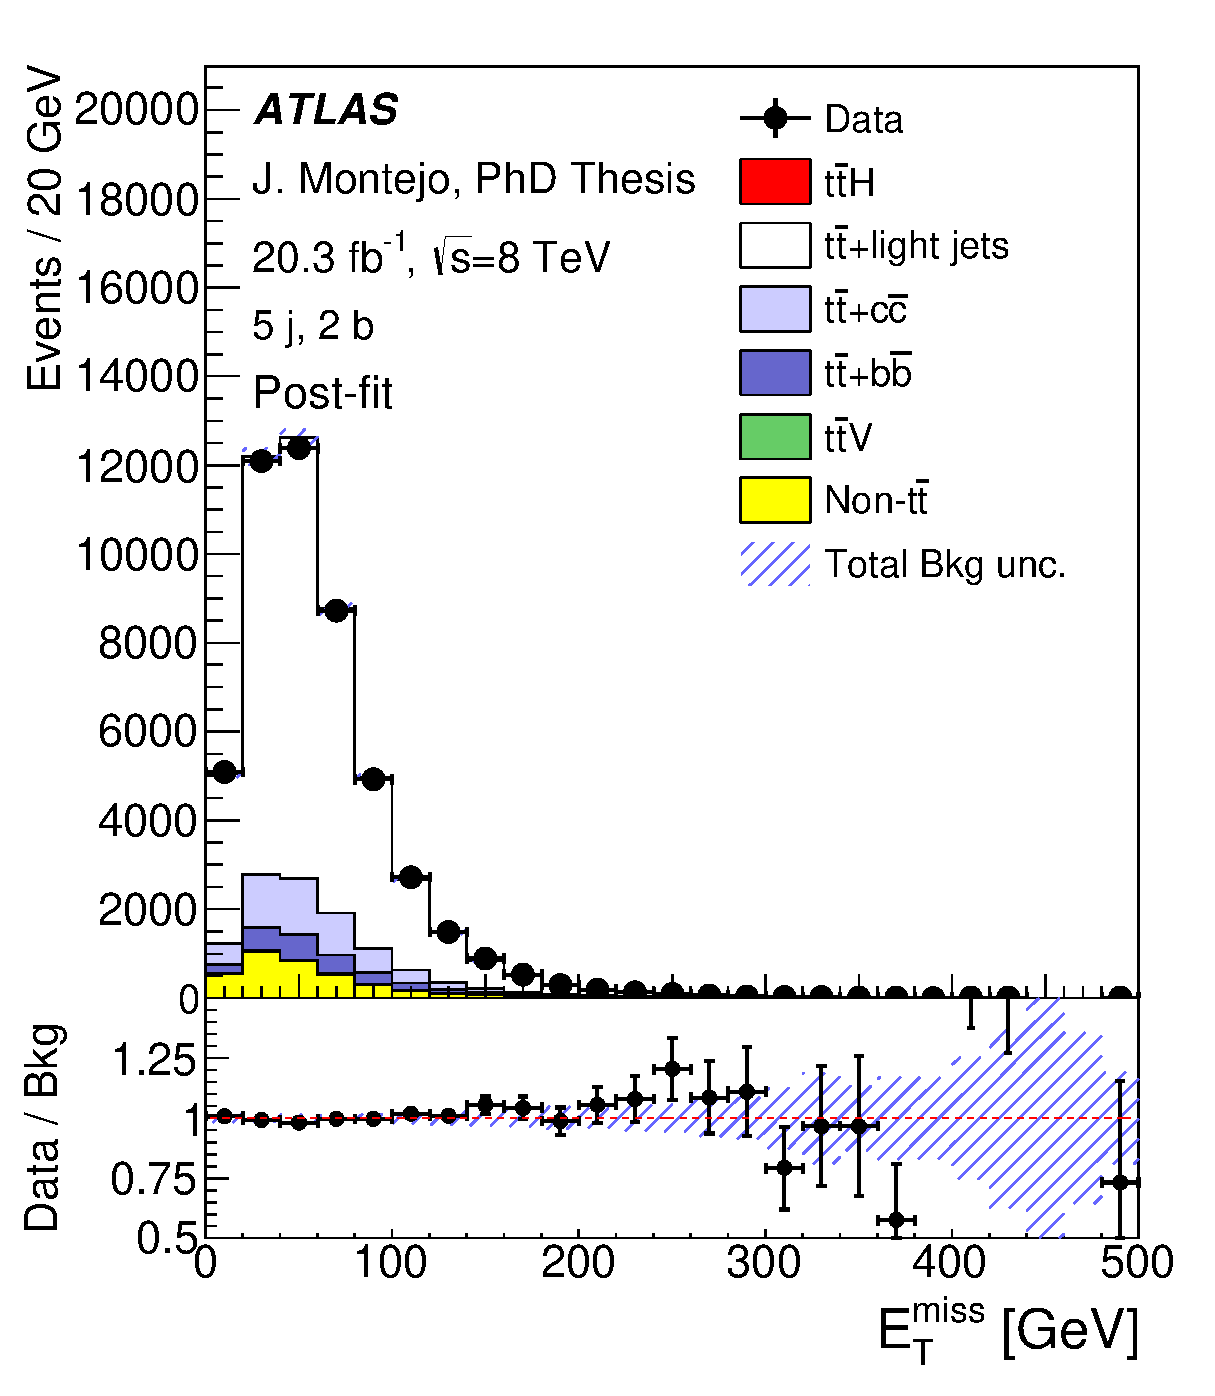
\includegraphics[width=0.27\textwidth]{Analysis/Figures_ttH/tesis_vars/postfit/met_5jetex2btagex.eps} &
  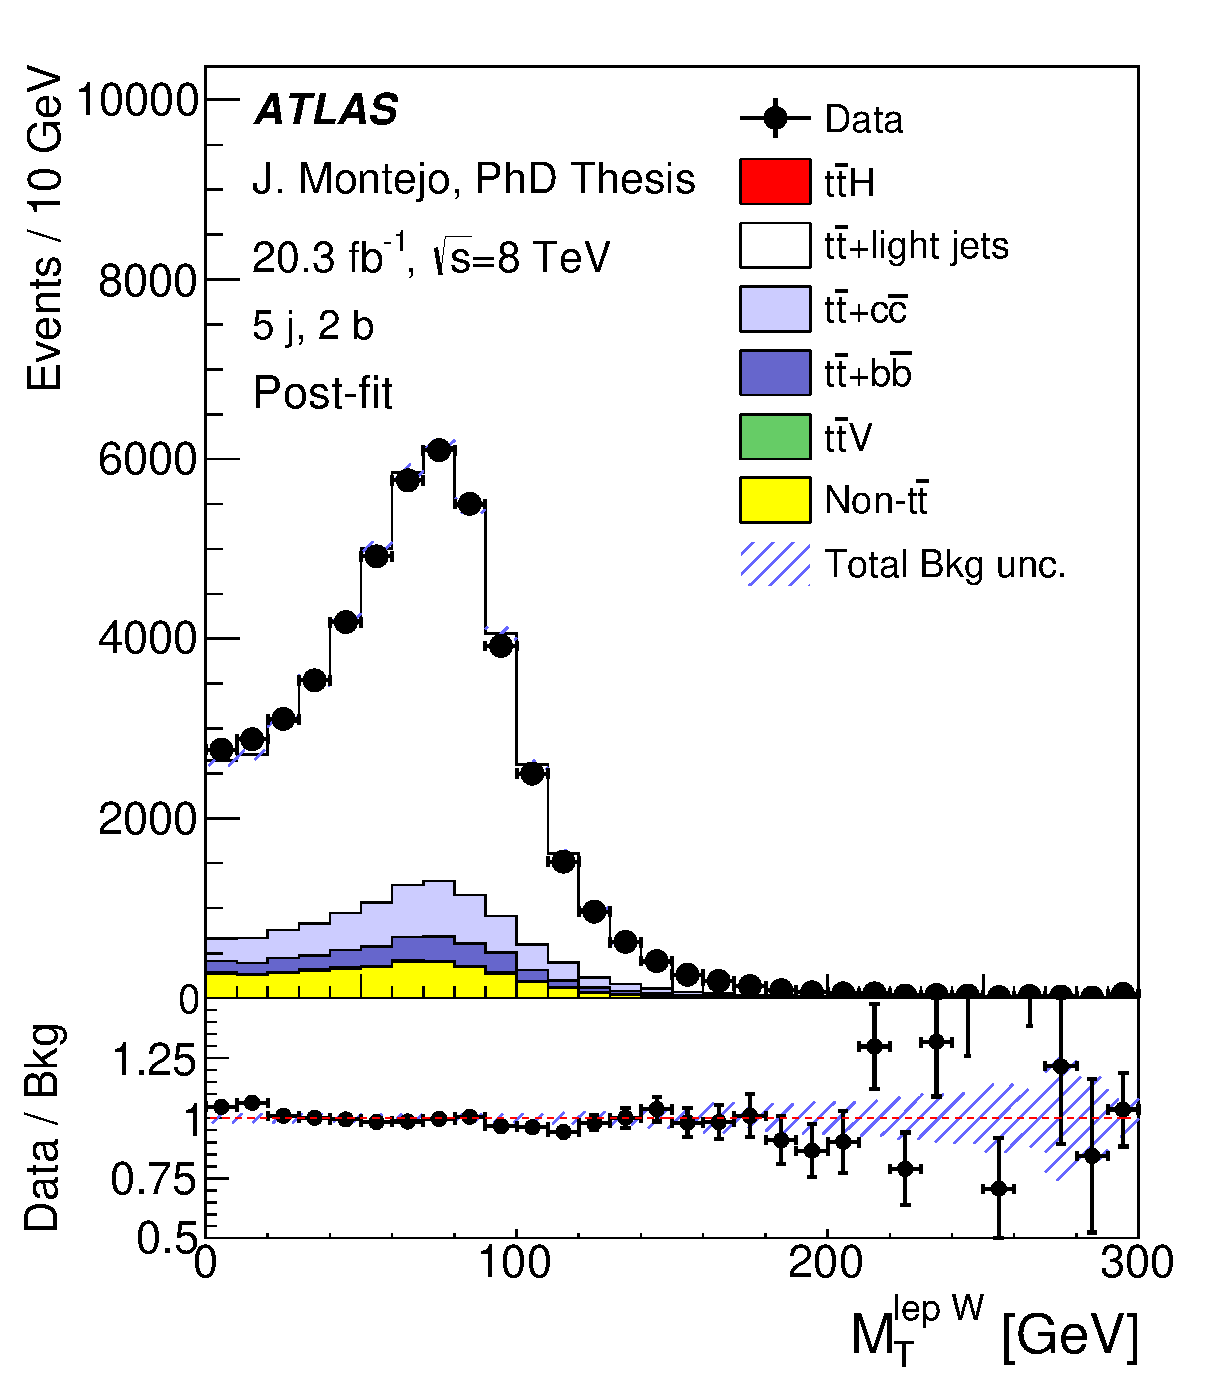
\includegraphics[width=0.27\textwidth]{Analysis/Figures_ttH/tesis_vars/postfit/WlepMT_5jetex2btagex.eps} \\
\end{tabular}
\caption{Comparison between data and prediction in the \fivetwo\ region for (left) lepton \pt,  (middle) missing transverse energy, \met, and (right)  $W$ boson transverse mass, \mtw. The background prediction is shown (top) before the fit and (bottom) after the fit.}
  \label{fig:vars1_fivetwo}
\vspace{0.5cm}
  \centering
  \begin{tabular}{ccc}
  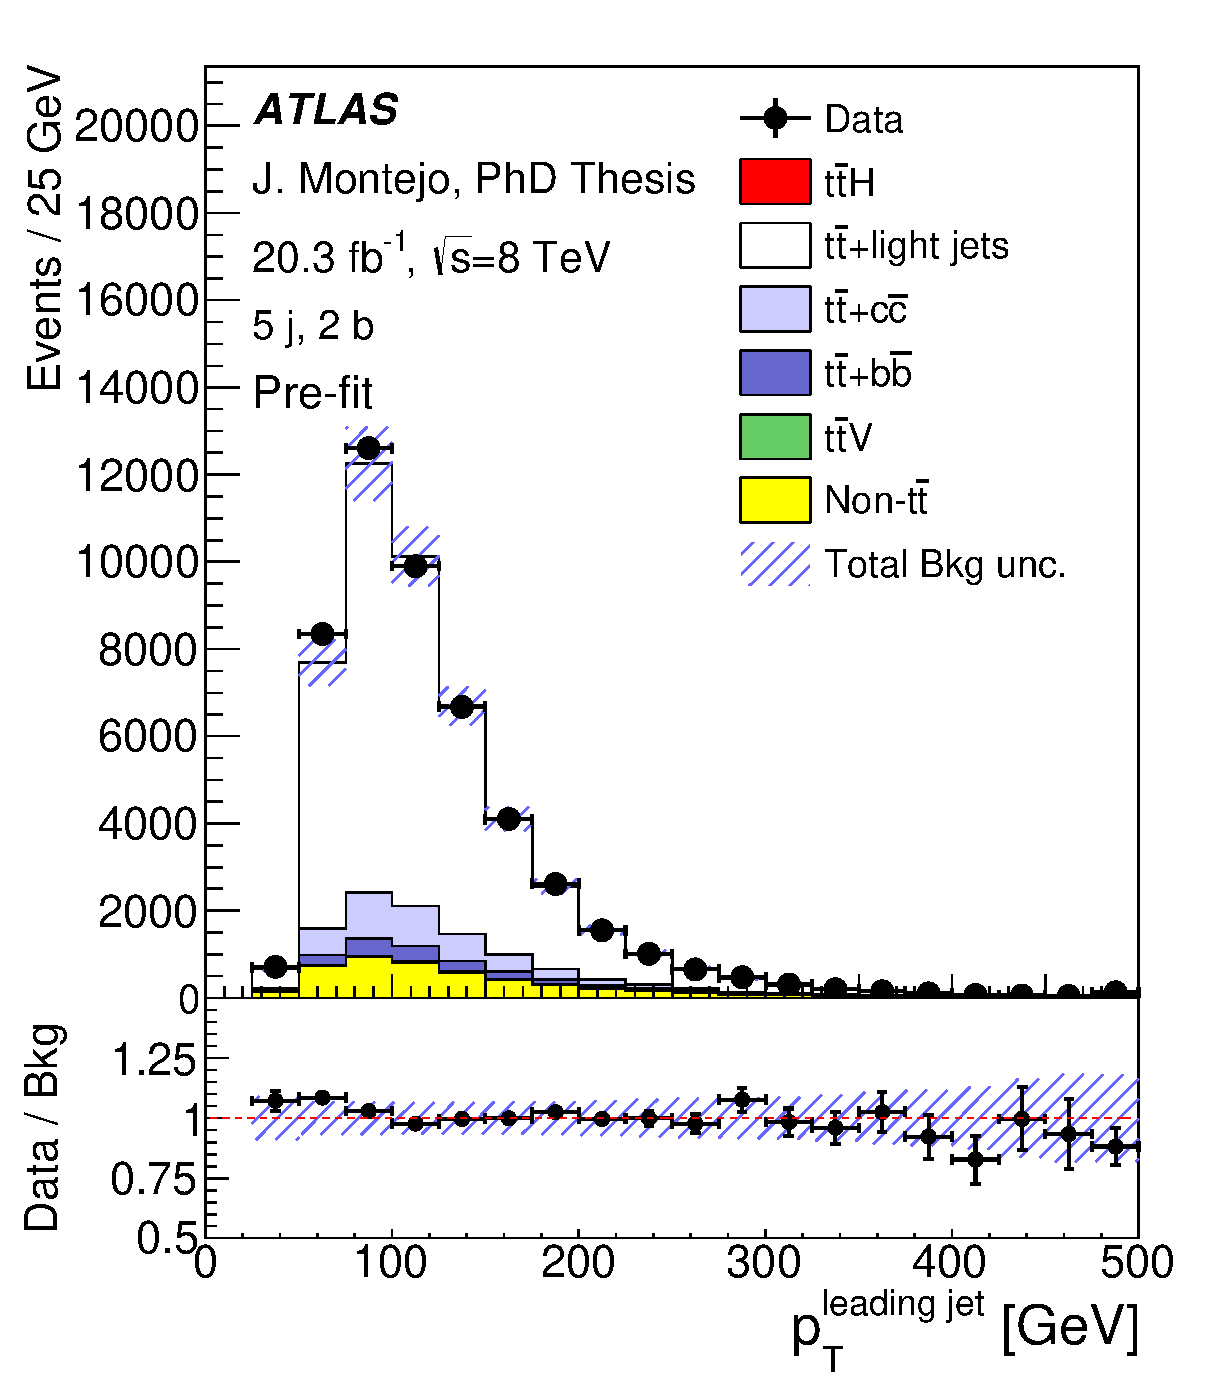
\includegraphics[width=0.27\textwidth]{Analysis/Figures_ttH/tesis_vars/prefit/jet1_pt_5jetex2btagex.eps} &
  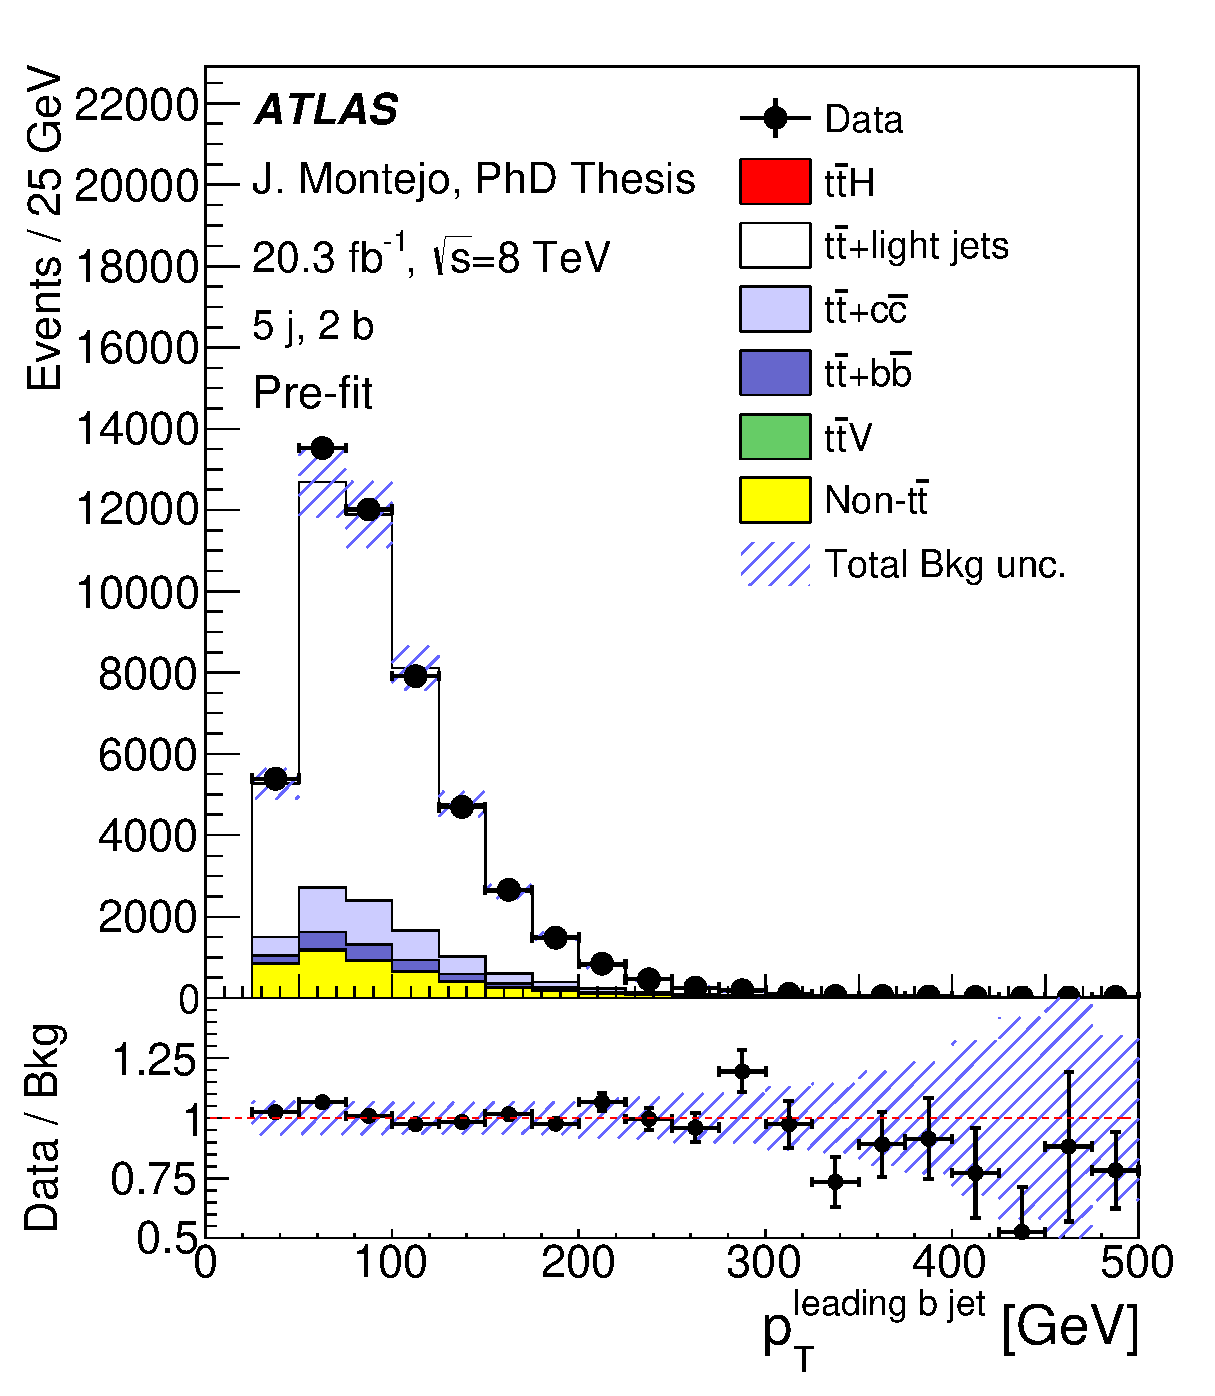
\includegraphics[width=0.27\textwidth]{Analysis/Figures_ttH/tesis_vars/prefit/bjet1_pt_5jetex2btagex.eps} &
  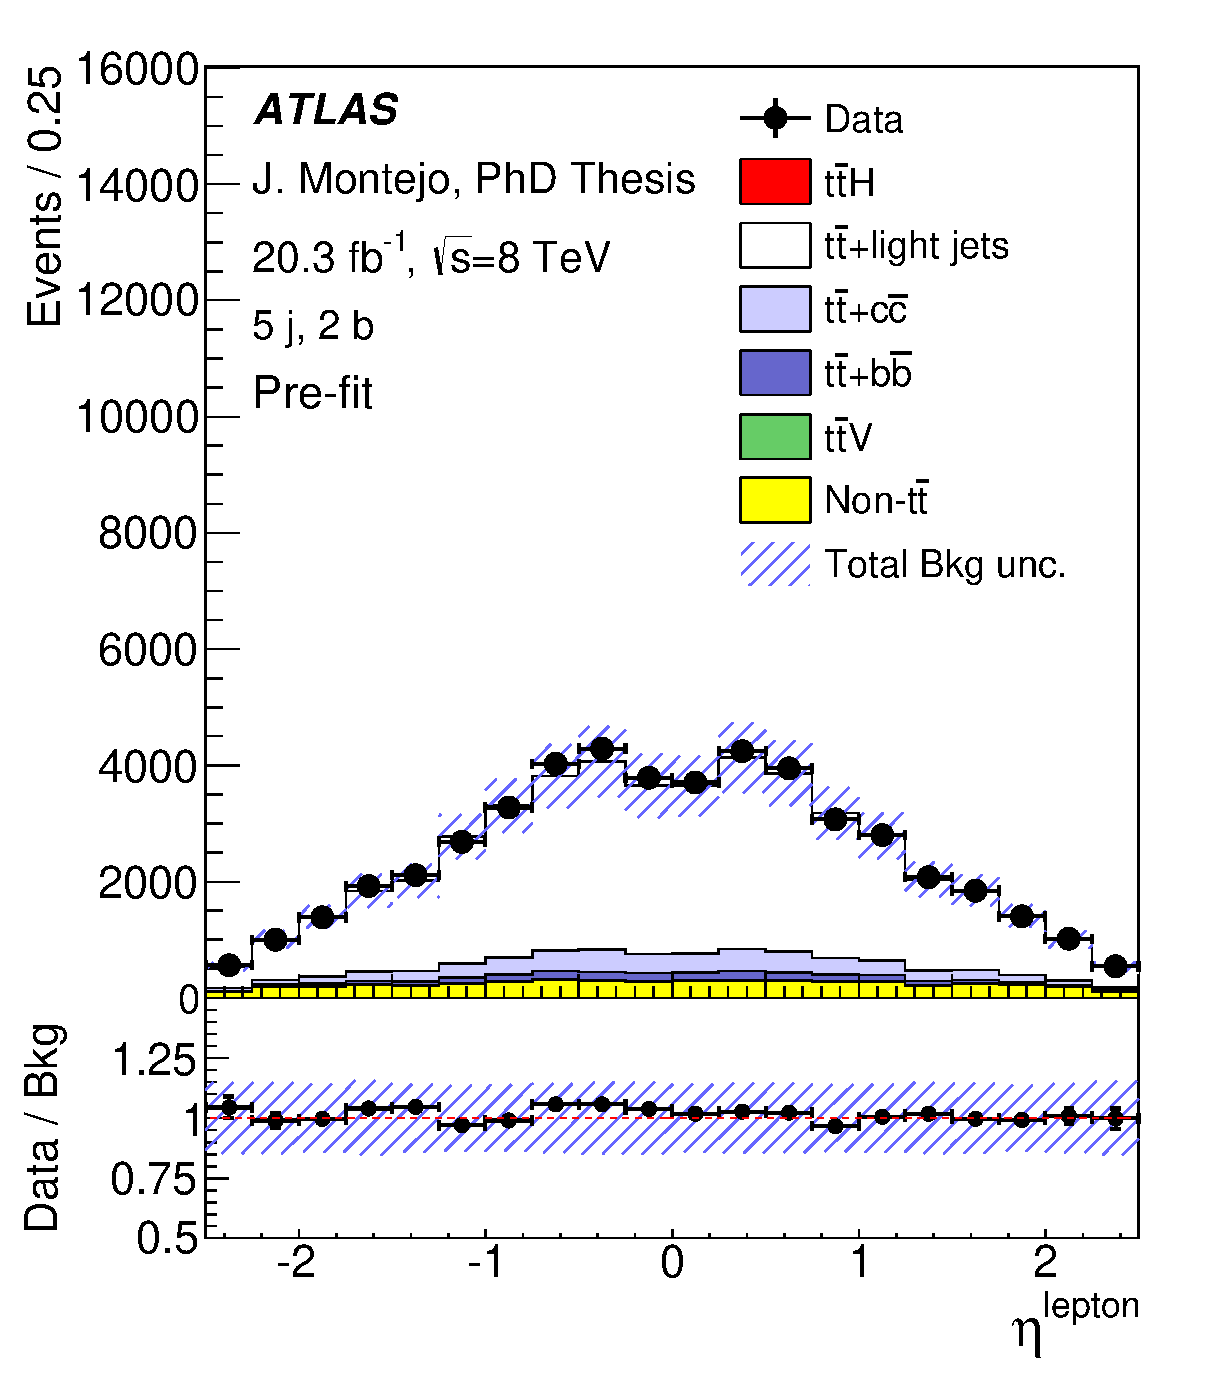
\includegraphics[width=0.27\textwidth]{Analysis/Figures_ttH/tesis_vars/prefit/lep_eta_5jetex2btagex.eps} \\
  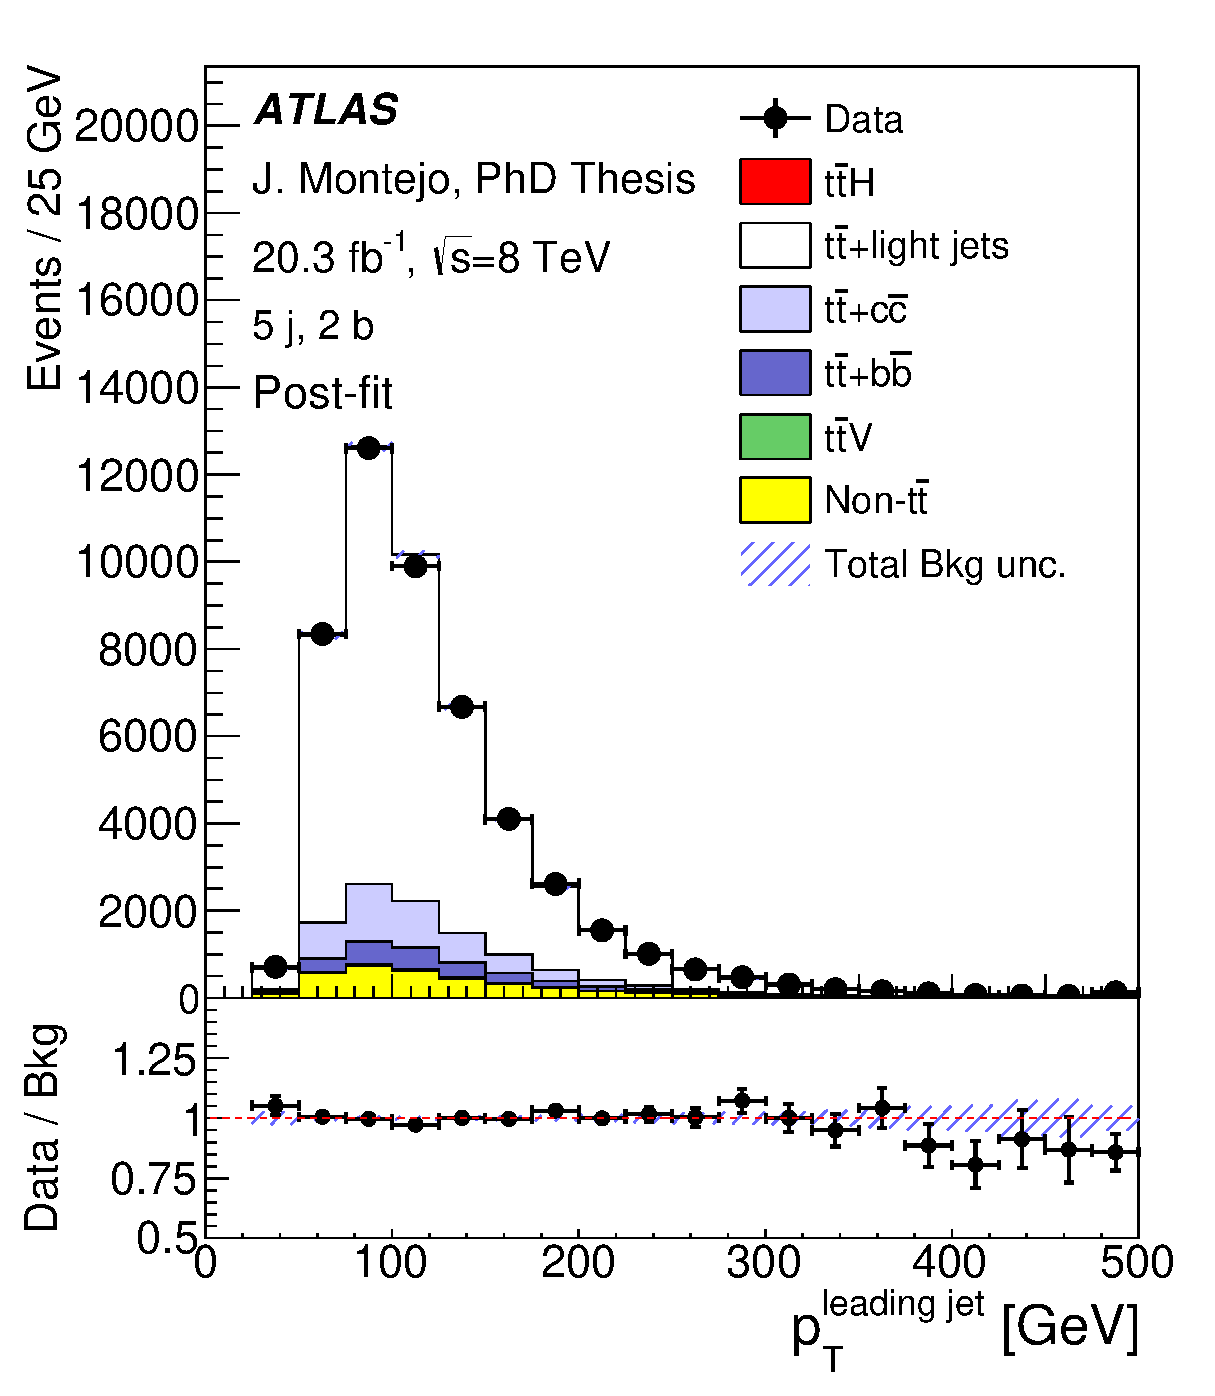
\includegraphics[width=0.27\textwidth]{Analysis/Figures_ttH/tesis_vars/postfit/jet1_pt_5jetex2btagex.eps} &
  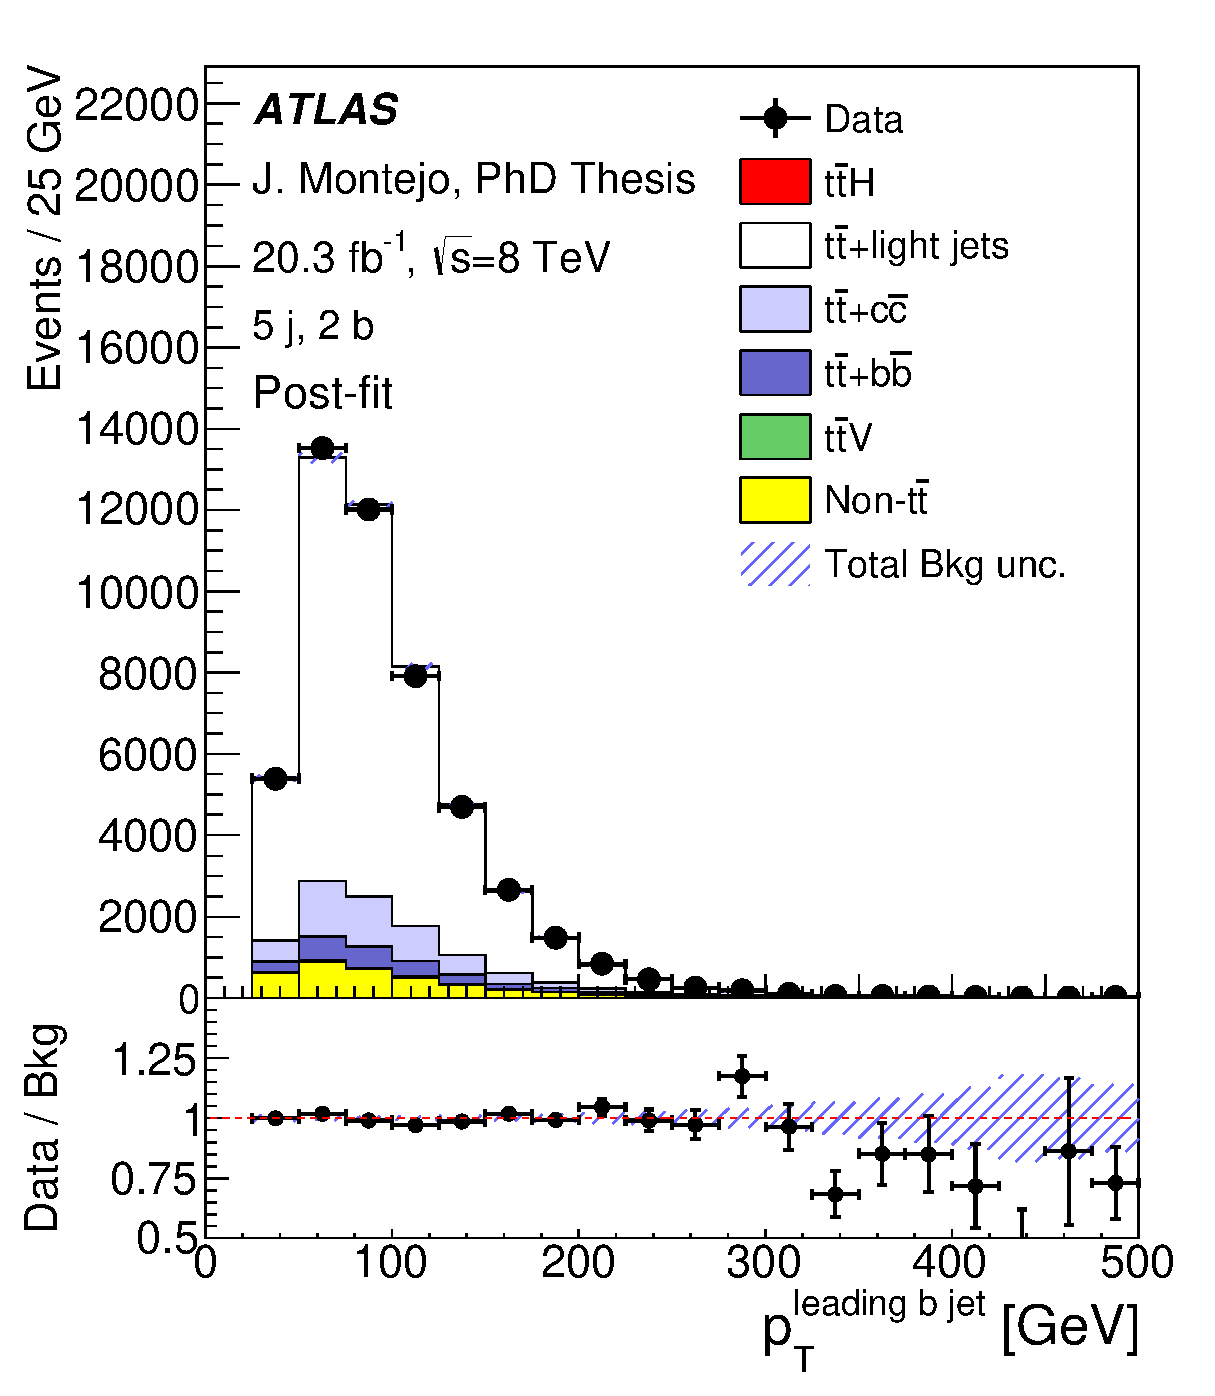
\includegraphics[width=0.27\textwidth]{Analysis/Figures_ttH/tesis_vars/postfit/bjet1_pt_5jetex2btagex.eps} &
  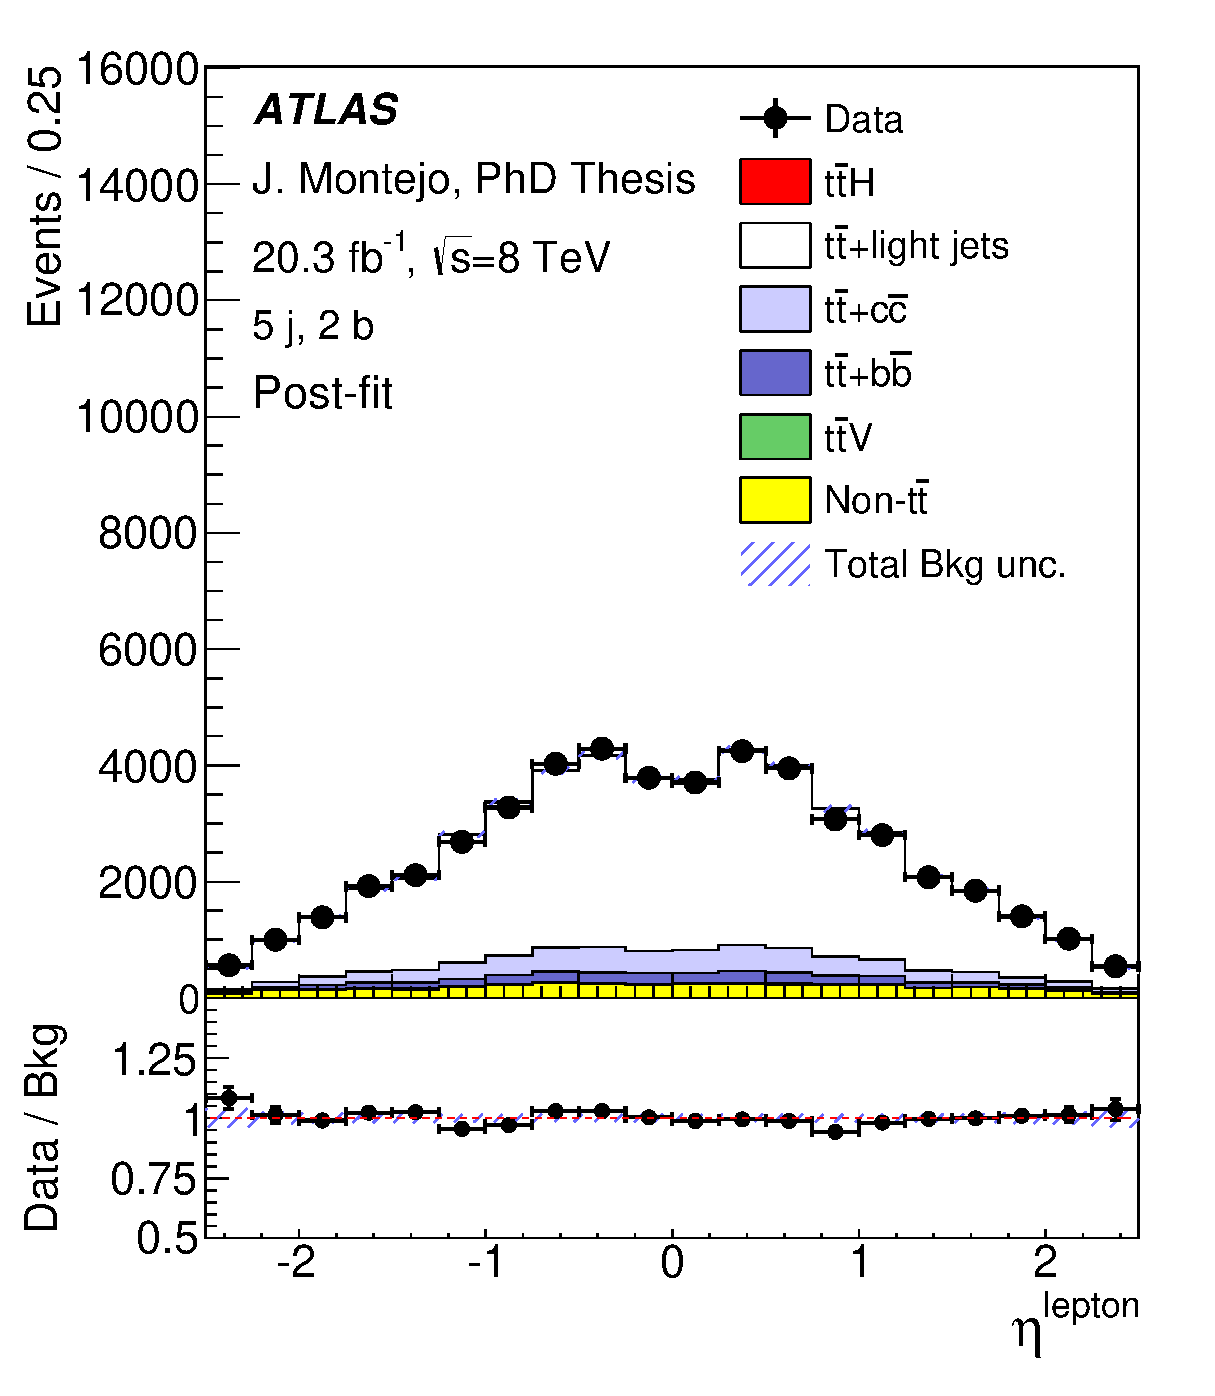
\includegraphics[width=0.27\textwidth]{Analysis/Figures_ttH/tesis_vars/postfit/lep_eta_5jetex2btagex.eps} \\
\end{tabular}
\caption{Comparison between data and prediction in the \fivetwo\ region for (left) leading jet \pt, (middle) leading $b$-tagged jet \pt, (right) lepton pseudo-rapidity. The background prediction is shown (top) before the fit and (bottom) after the fit.}
  \label{fig:vars2_fivetwo}
\end{figure}

\begin{figure}[tp]
  \centering
  \begin{tabular}{ccc}
  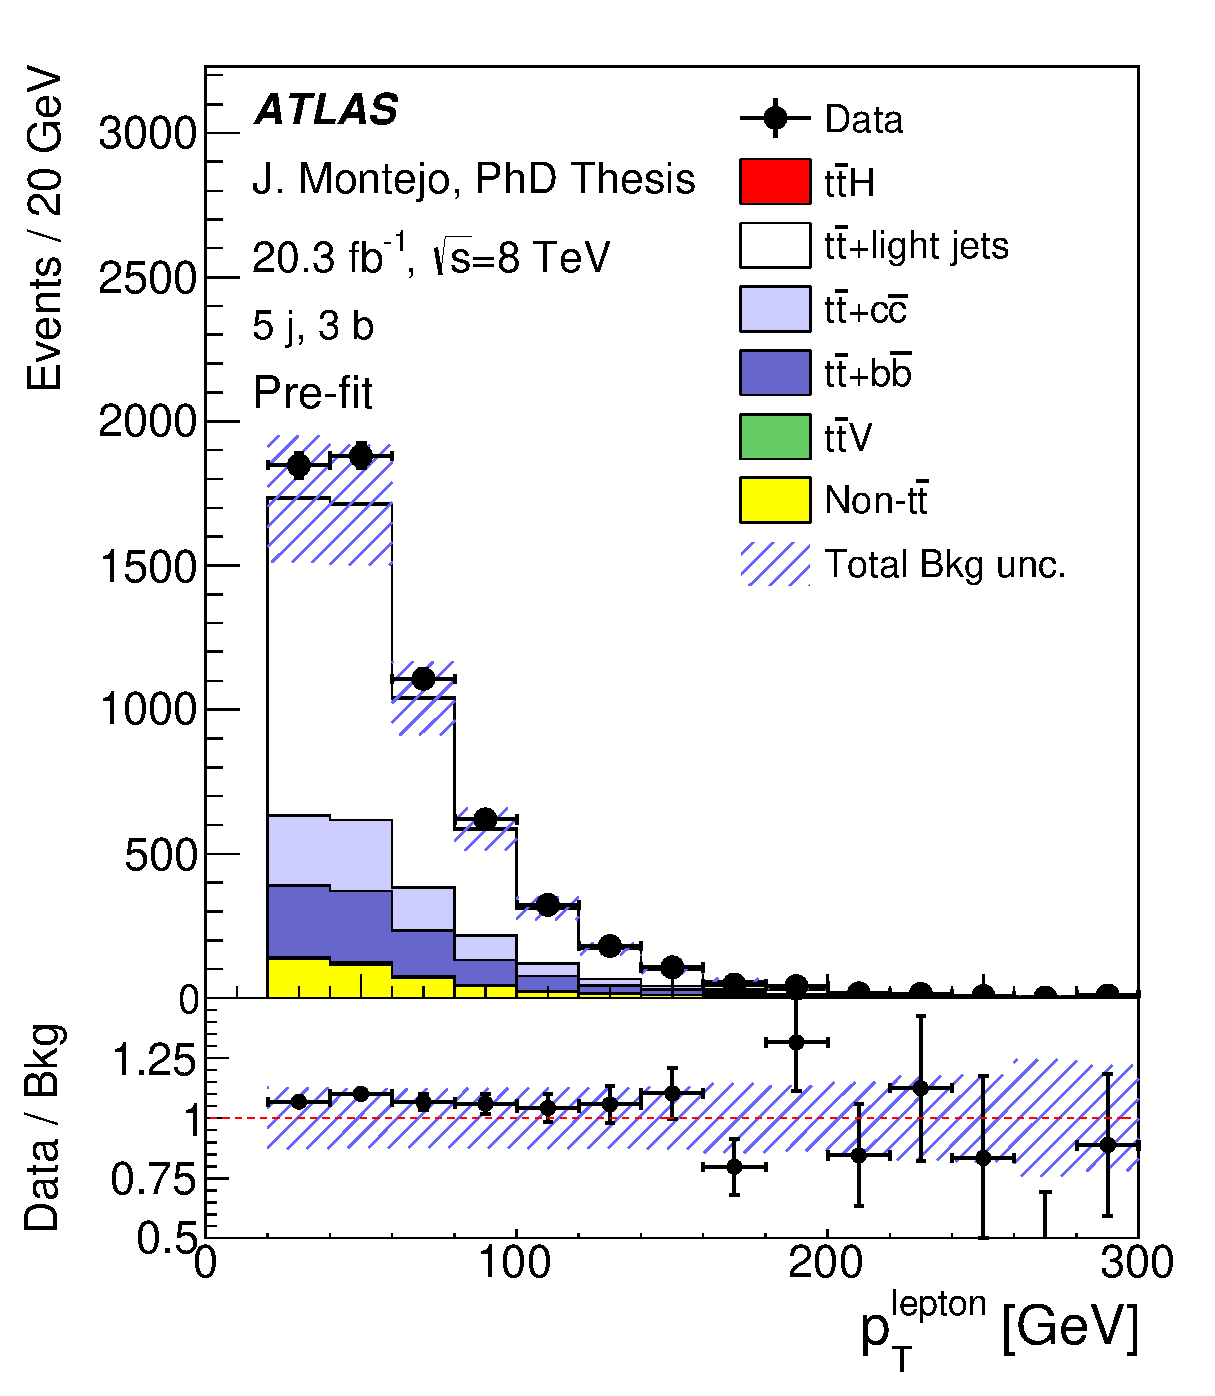
\includegraphics[width=0.27\textwidth]{Analysis/Figures_ttH/tesis_vars/prefit/lep_pt_5jetex3btagex.eps} &
  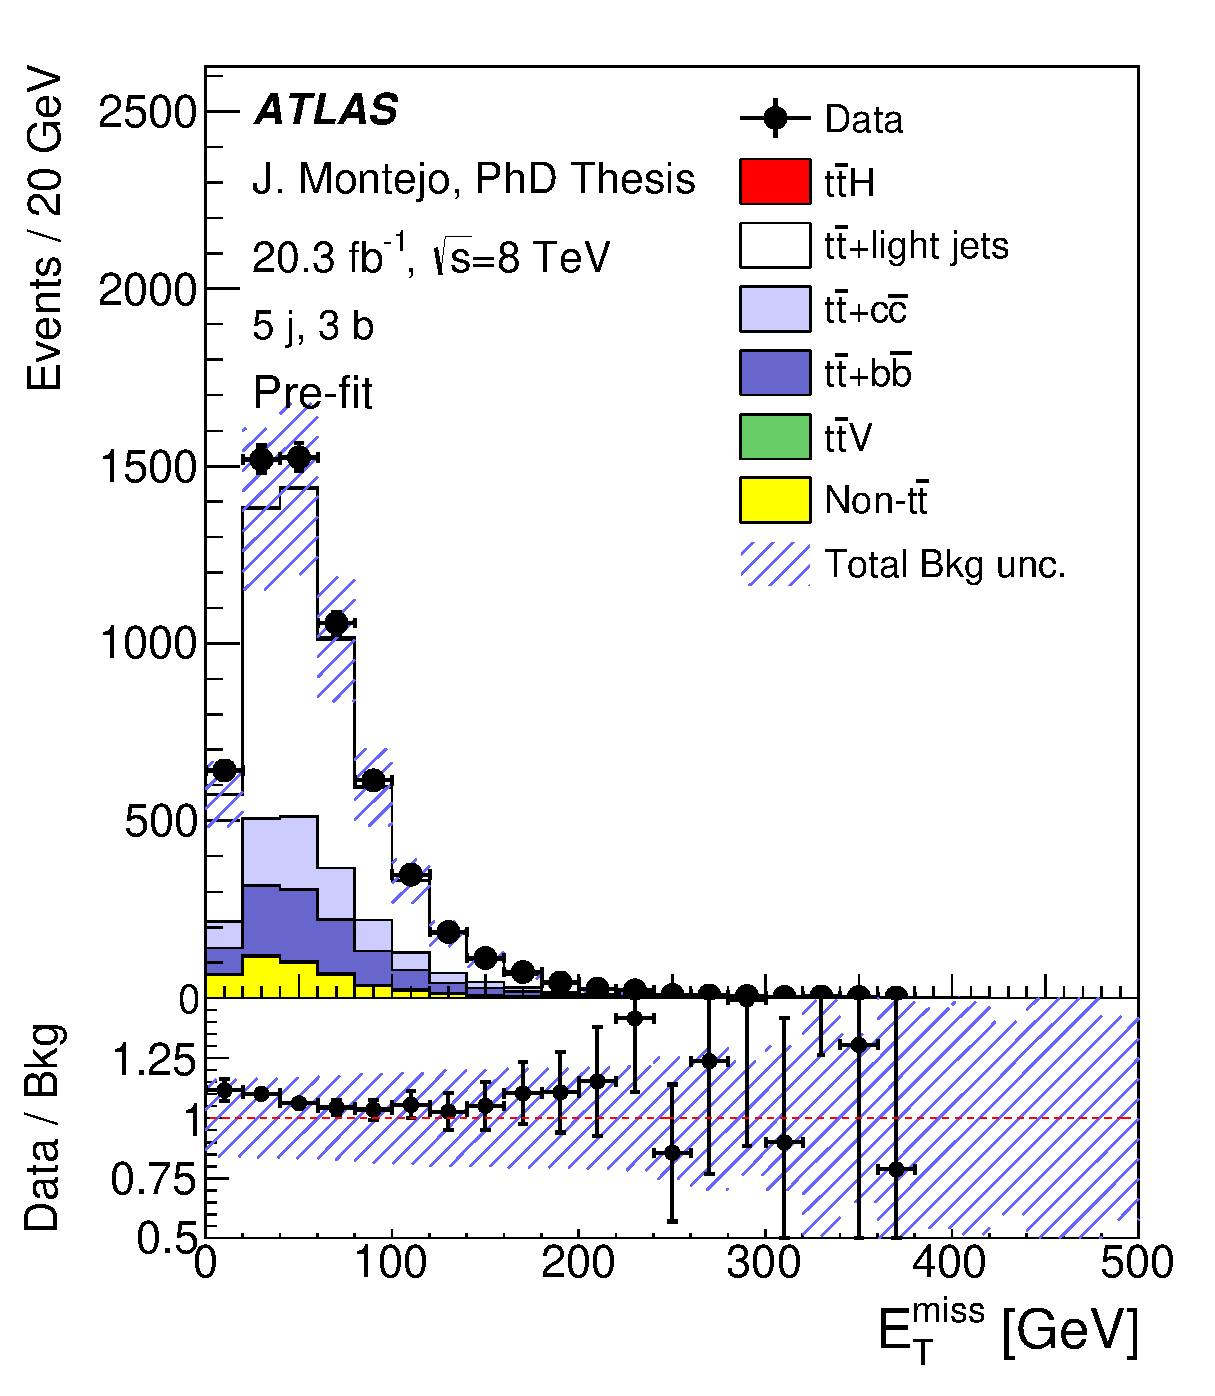
\includegraphics[width=0.27\textwidth]{Analysis/Figures_ttH/tesis_vars/prefit/met_5jetex3btagex.eps} &
  \includegraphics[width=0.27\textwidth]{Analysis/Figures_ttH/tesis_vars/prefit/WlepMT_5jetex3btagex.eps} \\
  \includegraphics[width=0.27\textwidth]{Analysis/Figures_ttH/tesis_vars/postfit/lep_pt_5jetex3btagex.eps} &
  \includegraphics[width=0.27\textwidth]{Analysis/Figures_ttH/tesis_vars/postfit/met_5jetex3btagex.eps} &
  \includegraphics[width=0.27\textwidth]{Analysis/Figures_ttH/tesis_vars/postfit/WlepMT_5jetex3btagex.eps} \\
\end{tabular}
\caption{Comparison between data and prediction in the \fivethree\ region for (left) lepton \pt,  (middle) missing transverse energy, \met, and (right)  $W$ boson transverse mass, \mtw. The background prediction is shown (top) before the fit and (bottom) after the fit.}
  \label{fig:vars1_fivethree}
\vspace{0.5cm}
  \centering
  \begin{tabular}{ccc}
  \includegraphics[width=0.27\textwidth]{Analysis/Figures_ttH/tesis_vars/prefit/jet1_pt_5jetex3btagex.eps} &
  \includegraphics[width=0.27\textwidth]{Analysis/Figures_ttH/tesis_vars/prefit/bjet1_pt_5jetex3btagex.eps} &
  \includegraphics[width=0.27\textwidth]{Analysis/Figures_ttH/tesis_vars/prefit/lep_eta_5jetex3btagex.eps} \\
  \includegraphics[width=0.27\textwidth]{Analysis/Figures_ttH/tesis_vars/postfit/jet1_pt_5jetex3btagex.eps} &
  \includegraphics[width=0.27\textwidth]{Analysis/Figures_ttH/tesis_vars/postfit/bjet1_pt_5jetex3btagex.eps} &
  \includegraphics[width=0.27\textwidth]{Analysis/Figures_ttH/tesis_vars/postfit/lep_eta_5jetex3btagex.eps} \\
\end{tabular}
\caption{Comparison between data and prediction in the \fivethree\ region for (left) leading jet \pt, (middle) leading $b$-tagged jet \pt, (right) lepton pseudo-rapidity. The background prediction is shown (top) before the fit and (bottom) after the fit.}
  \label{fig:vars2_fivethree}
\end{figure}
\begin{figure}[tp]
  \centering
  \begin{tabular}{ccc}
  \includegraphics[width=0.27\textwidth]{Analysis/Figures_ttH/tesis_vars/prefit/lep_pt_5jetex4btagin.eps} &
  \includegraphics[width=0.27\textwidth]{Analysis/Figures_ttH/tesis_vars/prefit/met_5jetex4btagin.eps} &
  \includegraphics[width=0.27\textwidth]{Analysis/Figures_ttH/tesis_vars/prefit/WlepMT_5jetex4btagin.eps} \\
  \includegraphics[width=0.27\textwidth]{Analysis/Figures_ttH/tesis_vars/postfit/lep_pt_5jetex4btagin.eps} &
  \includegraphics[width=0.27\textwidth]{Analysis/Figures_ttH/tesis_vars/postfit/met_5jetex4btagin.eps} &
  \includegraphics[width=0.27\textwidth]{Analysis/Figures_ttH/tesis_vars/postfit/WlepMT_5jetex4btagin.eps} \\
\end{tabular}
\caption{Comparison between data and prediction in the \fivefour\ region for (left) lepton \pt,  (middle) missing transverse energy, \met, and (right)  $W$ boson transverse mass, \mtw. The background prediction is shown (top) before the fit and (bottom) after the fit.}
  \label{fig:vars1_fivefour}
\vspace{0.5cm}
  \centering
  \begin{tabular}{ccc}
  \includegraphics[width=0.27\textwidth]{Analysis/Figures_ttH/tesis_vars/prefit/jet1_pt_5jetex4btagin.eps} &
  \includegraphics[width=0.27\textwidth]{Analysis/Figures_ttH/tesis_vars/prefit/bjet1_pt_5jetex4btagin.eps} &
  \includegraphics[width=0.27\textwidth]{Analysis/Figures_ttH/tesis_vars/prefit/lep_eta_5jetex4btagin.eps} \\
  \includegraphics[width=0.27\textwidth]{Analysis/Figures_ttH/tesis_vars/postfit/jet1_pt_5jetex4btagin.eps} &
  \includegraphics[width=0.27\textwidth]{Analysis/Figures_ttH/tesis_vars/postfit/bjet1_pt_5jetex4btagin.eps} &
  \includegraphics[width=0.27\textwidth]{Analysis/Figures_ttH/tesis_vars/postfit/lep_eta_5jetex4btagin.eps} \\
\end{tabular}
\caption{Comparison between data and prediction in the \fivefour\ region for (left) leading jet \pt, (middle) leading $b$-tagged jet \pt, (right) lepton pseudo-rapidity. The background prediction is shown (top) before the fit and (bottom) after the fit.}
  \label{fig:vars2_fivefour}
\end{figure}
\begin{figure}[tp]
  \centering
  \begin{tabular}{ccc}
  \includegraphics[width=0.27\textwidth]{Analysis/Figures_ttH/tesis_vars/prefit/lep_pt_6jetin2btagex.eps} &
  \includegraphics[width=0.27\textwidth]{Analysis/Figures_ttH/tesis_vars/prefit/met_6jetin2btagex.eps} &
  \includegraphics[width=0.27\textwidth]{Analysis/Figures_ttH/tesis_vars/prefit/WlepMT_6jetin2btagex.eps} \\
  \includegraphics[width=0.27\textwidth]{Analysis/Figures_ttH/tesis_vars/postfit/lep_pt_6jetin2btagex.eps} &
  \includegraphics[width=0.27\textwidth]{Analysis/Figures_ttH/tesis_vars/postfit/met_6jetin2btagex.eps} &
  \includegraphics[width=0.27\textwidth]{Analysis/Figures_ttH/tesis_vars/postfit/WlepMT_6jetin2btagex.eps} \\
\end{tabular}
\caption{Comparison between data and prediction in the \sixtwo\ region for (left) lepton \pt,  (middle) missing transverse energy, \met, and (right)  $W$ boson transverse mass, \mtw. The background prediction is shown (top) before the fit and (bottom) after the fit.}
  \label{fig:vars1_sixtwo}
\vspace{0.5cm}
  \centering
  \begin{tabular}{ccc}
  \includegraphics[width=0.27\textwidth]{Analysis/Figures_ttH/tesis_vars/prefit/jet1_pt_6jetin2btagex.eps} &
  \includegraphics[width=0.27\textwidth]{Analysis/Figures_ttH/tesis_vars/prefit/bjet1_pt_6jetin2btagex.eps} &
  \includegraphics[width=0.27\textwidth]{Analysis/Figures_ttH/tesis_vars/prefit/lep_eta_6jetin2btagex.eps} \\
  \includegraphics[width=0.27\textwidth]{Analysis/Figures_ttH/tesis_vars/postfit/jet1_pt_6jetin2btagex.eps} &
  \includegraphics[width=0.27\textwidth]{Analysis/Figures_ttH/tesis_vars/postfit/bjet1_pt_6jetin2btagex.eps} &
  \includegraphics[width=0.27\textwidth]{Analysis/Figures_ttH/tesis_vars/postfit/lep_eta_6jetin2btagex.eps} \\
\end{tabular}
\caption{Comparison between data and prediction in the \sixtwo\ region for (left) leading jet \pt, (middle) leading $b$-tagged jet \pt, (right) lepton pseudo-rapidity. The background prediction is shown (top) before the fit and (bottom) after the fit.}
  \label{fig:vars2_sixtwo}
\end{figure}

\begin{figure}[tp]
  \centering
  \begin{tabular}{ccc}
  \includegraphics[width=0.27\textwidth]{Analysis/Figures_ttH/tesis_vars/prefit/lep_pt_6jetin3btagex.eps} &
  \includegraphics[width=0.27\textwidth]{Analysis/Figures_ttH/tesis_vars/prefit/met_6jetin3btagex.eps} &
  \includegraphics[width=0.27\textwidth]{Analysis/Figures_ttH/tesis_vars/prefit/WlepMT_6jetin3btagex.eps} \\
  \includegraphics[width=0.27\textwidth]{Analysis/Figures_ttH/tesis_vars/postfit/lep_pt_6jetin3btagex.eps} &
  \includegraphics[width=0.27\textwidth]{Analysis/Figures_ttH/tesis_vars/postfit/met_6jetin3btagex.eps} &
  \includegraphics[width=0.27\textwidth]{Analysis/Figures_ttH/tesis_vars/postfit/WlepMT_6jetin3btagex.eps} \\
\end{tabular}
\caption{Comparison between data and prediction in the \sixthree\ region for (left) lepton \pt,  (middle) missing transverse energy, \met, and (right)  $W$ boson transverse mass, \mtw. The background prediction is shown (top) before the fit and (bottom) after the fit.}
  \label{fig:vars1_sixthree}
\vspace{0.5cm}
  \centering
  \begin{tabular}{ccc}
  \includegraphics[width=0.27\textwidth]{Analysis/Figures_ttH/tesis_vars/prefit/jet1_pt_6jetin3btagex.eps} &
  \includegraphics[width=0.27\textwidth]{Analysis/Figures_ttH/tesis_vars/prefit/bjet1_pt_6jetin3btagex.eps} &
  \includegraphics[width=0.27\textwidth]{Analysis/Figures_ttH/tesis_vars/prefit/lep_eta_6jetin3btagex.eps} \\
  \includegraphics[width=0.27\textwidth]{Analysis/Figures_ttH/tesis_vars/postfit/jet1_pt_6jetin3btagex.eps} &
  \includegraphics[width=0.27\textwidth]{Analysis/Figures_ttH/tesis_vars/postfit/bjet1_pt_6jetin3btagex.eps} &
  \includegraphics[width=0.27\textwidth]{Analysis/Figures_ttH/tesis_vars/postfit/lep_eta_6jetin3btagex.eps} \\
\end{tabular}
\caption{Comparison between data and prediction in the \sixthree\ region for (left) leading jet \pt, (middle) leading $b$-tagged jet \pt, (right) lepton pseudo-rapidity. The background prediction is shown (top) before the fit and (bottom) after the fit.}
  \label{fig:vars2_sixthree}
\end{figure}

\begin{figure}[tp]
  \centering
  \begin{tabular}{ccc}
  \includegraphics[width=0.27\textwidth]{Analysis/Figures_ttH/tesis_vars/prefit/lep_pt_6jetin4btagin.eps} &
  \includegraphics[width=0.27\textwidth]{Analysis/Figures_ttH/tesis_vars/prefit/met_6jetin4btagin.eps} &
  \includegraphics[width=0.27\textwidth]{Analysis/Figures_ttH/tesis_vars/prefit/WlepMT_6jetin4btagin.eps} \\
  \includegraphics[width=0.27\textwidth]{Analysis/Figures_ttH/tesis_vars/postfit/lep_pt_6jetin4btagin.eps} &
  \includegraphics[width=0.27\textwidth]{Analysis/Figures_ttH/tesis_vars/postfit/met_6jetin4btagin.eps} &
  \includegraphics[width=0.27\textwidth]{Analysis/Figures_ttH/tesis_vars/postfit/WlepMT_6jetin4btagin.eps} \\
\end{tabular}
\caption{Comparison between data and prediction in the \sixfour\ region for (left) lepton \pt,  (middle) missing transverse energy, \met, and (right)  $W$ boson transverse mass, \mtw. The background prediction is shown (top) before the fit and (bottom) after the fit.}
  \label{fig:vars1_sixfour}
\vspace{0.5cm}
  \centering
  \begin{tabular}{ccc}
  \includegraphics[width=0.27\textwidth]{Analysis/Figures_ttH/tesis_vars/prefit/jet1_pt_6jetin4btagin.eps} &
  \includegraphics[width=0.27\textwidth]{Analysis/Figures_ttH/tesis_vars/prefit/bjet1_pt_6jetin4btagin.eps} &
  \includegraphics[width=0.27\textwidth]{Analysis/Figures_ttH/tesis_vars/prefit/lep_eta_6jetin4btagin.eps} \\
  \includegraphics[width=0.27\textwidth]{Analysis/Figures_ttH/tesis_vars/postfit/jet1_pt_6jetin4btagin.eps} &
  \includegraphics[width=0.27\textwidth]{Analysis/Figures_ttH/tesis_vars/postfit/bjet1_pt_6jetin4btagin.eps} &
  \includegraphics[width=0.27\textwidth]{Analysis/Figures_ttH/tesis_vars/postfit/lep_eta_6jetin4btagin.eps} \\
\end{tabular}
\caption{Comparison between data and prediction in the \sixfour\ region for (left) leading jet \pt, (middle) leading $b$-tagged jet \pt, (right) lepton pseudo-rapidity. The background prediction is shown (top) before the fit and (bottom) after the fit.}
  \label{fig:vars2_sixfour}
\end{figure}
